\documentclass[12pt,a4paper,russian,hidelinks]{report}     


%\usepackage{extsizes}
\usepackage{verbatim}
\usepackage{pdflscape}
\usepackage{subcaption}
\usepackage{indentfirst}
\usepackage{cmap} %чтобы работал поиск по кириллице
\usepackage{graphicx}
\graphicspath{ {./figures/} }
\DeclareGraphicsExtensions{.eps,.png,.jpg,.pdf}


\usepackage{hyperref}
\usepackage{float}
\usepackage{url}
\usepackage{amsmath}
\usepackage[utf8]{inputenc}
\usepackage[T2A]{fontenc}
\usepackage[russian]{babel}
\usepackage{multirow}
\usepackage[table]{xcolor}
\usepackage{tabu}
\usepackage{geometry}
\usepackage{caption}
\geometry{
	top = 20mm,
	left = 20mm,
	right = 20mm,
	bottom = 20mm
}
\selectlanguage{russian}
\hyphenation{БПЛА}
\hyphenation{ЦАГИ}

\newcommand{\m}{\text{м}}
\newcommand{\kgs}{\text{кгс}}
\renewcommand{\thesubfigure}{\asbuk{subfigure}}


\begin{document}
\begin{titlepage}
\newpage		

\begin{center}
ФЕДЕРАЛЬНОЕ АГЕНТСТВО ПО ОБРАЗОВАНИЮ РФ \\
\vspace{1cm}
МОСКОВСКИЙ ФИЗИКО-ТЕХНИЧЕСКИЙ ИНСТИТУТ \\*
(ГОСУДАРСТВЕННЫЙ УНИВЕРСИТЕТ) \\*
\hrulefill
\end{center}
 
\flushright{Кафедра Прочности Летательных Аппаратов}
\vspace{8em}

\begin{center}
\Large Дипломная работа на степень бакалавра на тему:
\end{center}

\vspace{2.5em}
 
\begin{center}
\textsc{\textbf{Исследование прочности конструкции центроплана \\ для крыльев большого удлинения.}}
\end{center}

\vspace{6em}
 
\begin{flushleft}
Студент\hrulefill ~Дынников~Ю.А. \\
\vspace{1.5em}
Научный руководитель \\
степень? \hrulefill ~Шаныгин~ А.Н.\\
\vspace{1.5em}
\vspace{1.5em}
Зав. кафедрой\\
степень? \hrulefill ~Замула~Г.Н.
\end{flushleft}
 
\vspace{\fill}

\begin{center}
Жуковский 2014
\end{center}

\end{titlepage}

\maketitle
\tableofcontents
\chapter*{Введение}

В настоящее время как в нашей стране, так и за рубежом всё большее внимание уделяется созданию различных типов беспилотных летательных аппаратов (БПЛА)~\cite{UAVBook}. 


В настоящее время разработаны и практически реализованы проекты БПЛА, предназначенные для решения различного рода задач как для гражданских, так и для военных целей. На Рис.\ref{fig:UAVs} представлены некоторые из существующих БПЛА с указанием их предназначения.


\begin{figure}[H]
        \begin{subfigure}[b]{0.47\textwidth}
                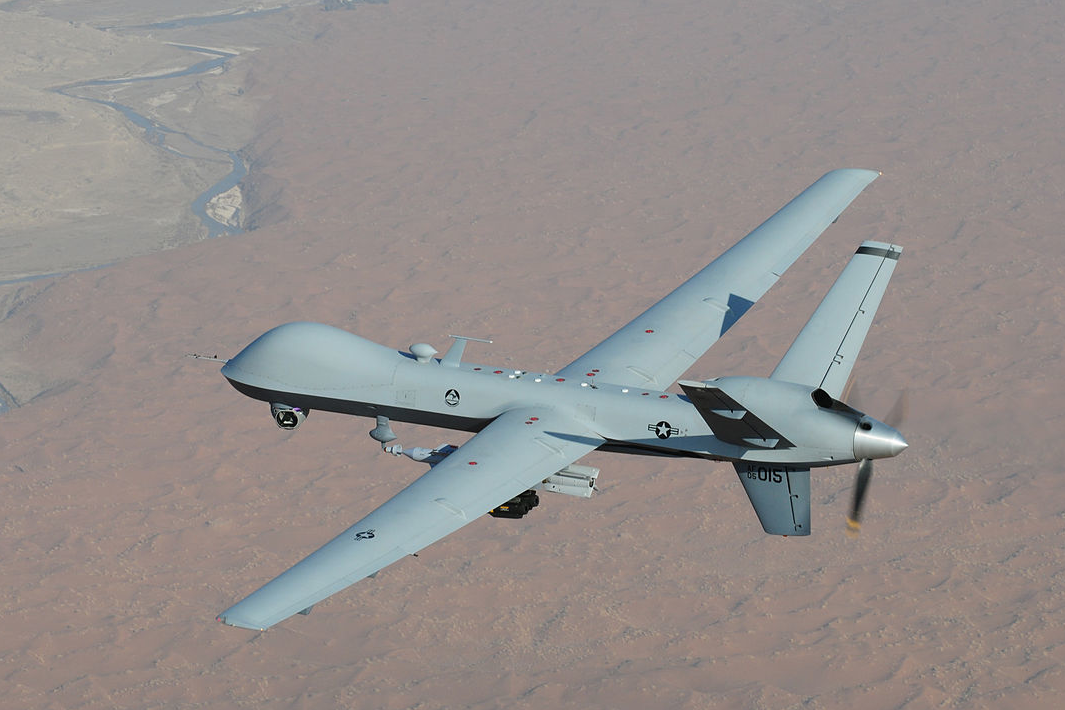
\includegraphics[width=\linewidth]{UAV_Reaper}
                \caption{MQ-9 Reaper, разведывательно-ударный} % http://ru.wikipedia.org/wiki/MQ-9_Reaper , U.S. Air Force Photo / Lt. Col. Leslie Pratt - USAF Photographic Archives http://www.afrc.af.mil/shared/media/photodb/photos/090127-F-7383P-002.JPG
                \label{fig:UAV_Reaper}
        \end{subfigure}%
        \hspace{\fill}
        \begin{subfigure}[b]{0.47\textwidth}
                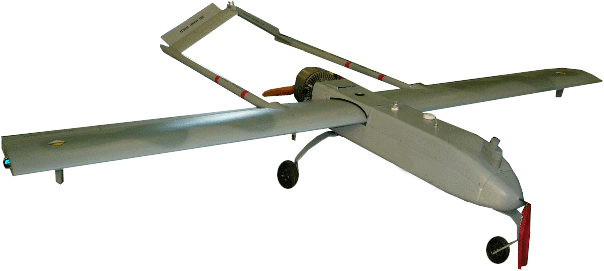
\includegraphics[width=\linewidth]{UAV_RQ7}
                \caption{RQ-7A Shadow 200, разведывательный}
                \label{fig:UAV_RQ7}
        \end{subfigure}
        \caption{Примеры существующих БПЛА}\label{fig:UAVs}
\end{figure}

Для решения многих практических задач (воздушные разведка и наблюдение, обеспечение связи и мониторинг состояния, доставка и десантирование грузов) использование беспилотных летательных аппаратов может обеспечить преимущество в стоимости эксплуатации и в достижении технических показателей по сравнению с пилотируемыми ЛА. Это связано с тем обстоятельством, что беспилотные ЛА проектируются с учетом других требований и ограничений, в частности для них:

\begin{itemize}
\item установлены существенно менее жесткие требования по безопасности конструкции;
\item не требуется систем поддержания работоспособности и жизнеобеспечения экипажа;
\item установлены существенно менее жесткие ограничения на области режимов полета.
\end{itemize} 

%При их создании особое внимание уделяется требованиям малозаметности и увеличения аэродинамического качества, и как следствие, возможности барражировать в течение длительного времени. 


Благодаря этому БПЛА имеют большой потенциал для разработки для них легких и дешевых конструкций планера, что позволяет решать многие технические задачи, недоступные для пилотируемых летательных аппаратов.




%Рассказать про беспилотник (типы, картинки), предназначены для решения ряда задач.

%Дальше про разные типы.


Как было сказано выше, одной из основных задач беспилотных самолетов является воздушные разведка и наблюдение. Такие самолеты предназначены для продолжительного (до 36 часов для RQ-4 ``Global Hawk'') барражирования без дозаправки, что накладывает на конструкцию самолета высокие требования к весовой эффективности и к аэродинамическому качеству.

%Основное - мониторинг (военный, гражданский). Из этого следуют требования малозаметности и весовой эффективности.

%Использование беспилотника может обеспечить преимущество по сравнению с пилотируемыми, почему.

%Показать несколько существующих и разрабатываемых БПЛА для мониторинга.

Для БПЛА, предназначенных для выполнения военных задач, большую роль также играет малозаметность БПЛА. Требования высоких аэродинамических характеристик и малозаметности накладывают на конструкцию БПЛА ряд ограничений на геометрические параметры; в частности конструкция БПЛА должна иметь минимально возможную строительную высоту, а также иметь обтекаемые обводы. (примеры таких БПЛА приведены на Рис.\ref{fig:UAVs_stealth}). Для достижения высокого аэродинамического качества  конструкция должна иметь крыло большого удлинения, интегрированное с несущим фюзеляжем. Использование крыльев большого удлинения влечет за собой появление больших изгибающих моментов в корневой части крыла и в центроплане. 


\begin{figure}[ht]
        \begin{subfigure}[b]{0.47\textwidth}
                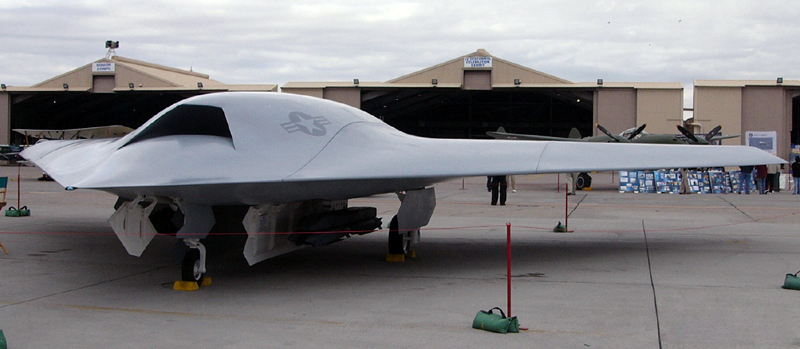
\includegraphics[width=\linewidth]{UAV_X45}
                \caption{Boeing X-45C, экспериментальный многоцелевой}
%http://ru.wikipedia.org/wiki/Boeing_X-45
                \label{fig:UAV_X45}
        \end{subfigure}%
        \hspace{\fill}
        \begin{subfigure}[b]{0.47\textwidth}
                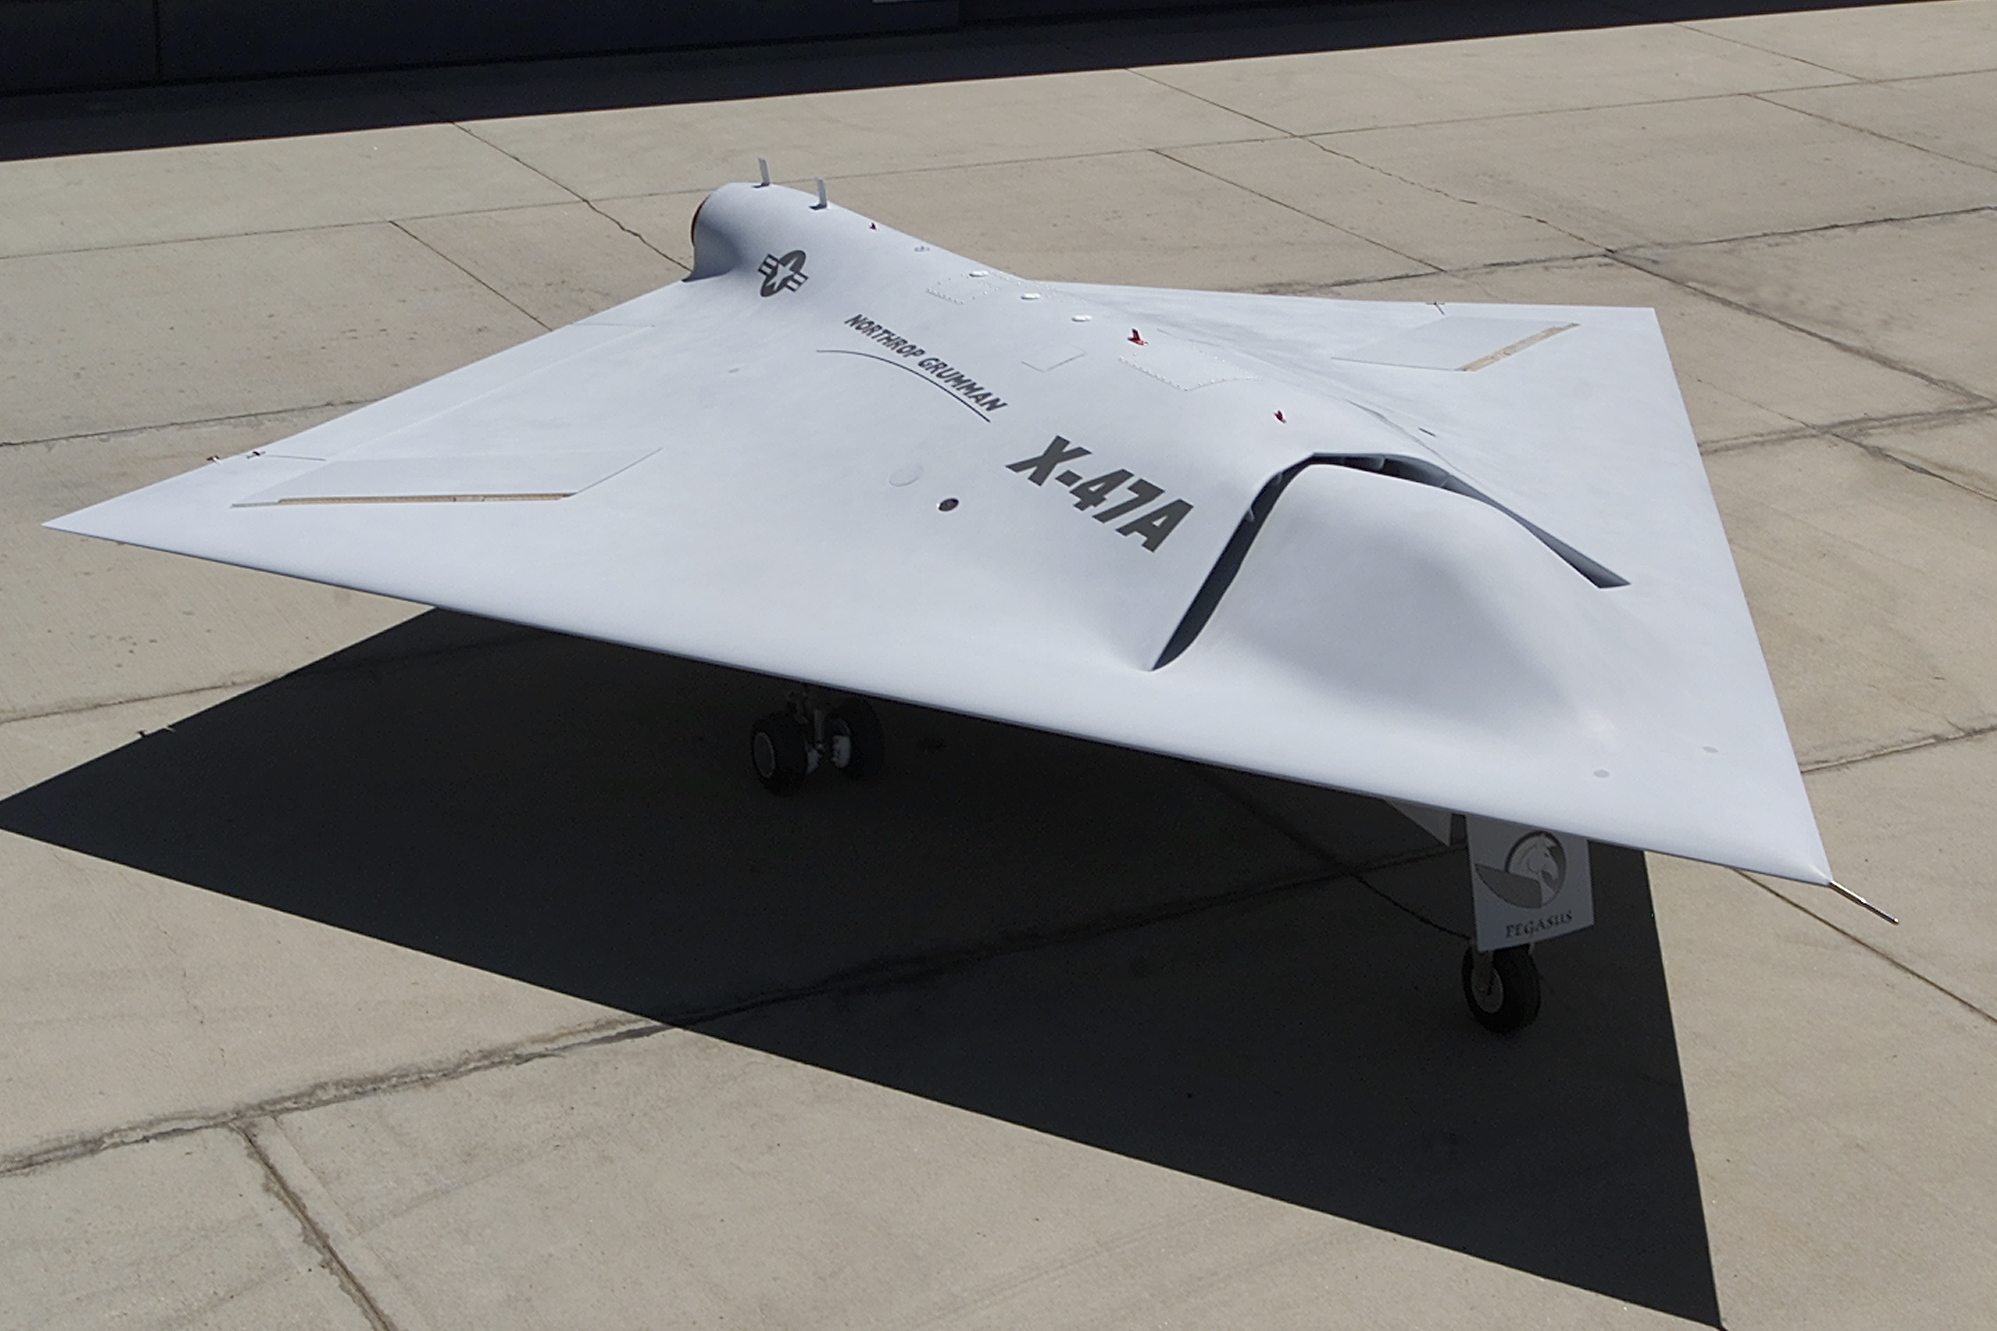
\includegraphics[width=\linewidth]{UAV_X47}
                \caption{Northrop X-47A, боевой} %http://ru.wikipedia.org/wiki/X-47_Pegasus
%		%http://archive.darpa.mil/j-ucas/X-47/gallery/X-47A/hi_res/pegasus2_hi-res.jpg
                \label{fig:UAV_X47}
        \end{subfigure}%
        \caption{БПЛА, выполненные по схеме ``Стелс''}\label{fig:UAVs_stealth}
\end{figure}
%Объясняем, почему нужна интегральная схема и крыло большого удлинения. Цель - меньше заметности следовательно уменьшение строительной высоты, больше аэродинамического качество.

Необходимость уменьшения строительной высоты БПЛА в свою очередь приводит к возникновению проблемы интеграции двигателя и центроплана. Одним из вариантов  решения такой интаграционной задачи является компоновочная схема БПЛА-ЦАГИ, разработанная в НИО-3, в которой двигатель с воздухозаборником максимально утоплен в конструкции корпуса БПЛА.
На Рис.\ref{fig:BPS} показана центральная часть (кабина) данного ЛА. Компоновка БПЛА-ЦАГИ показала хорошие аэродинамические характеристики и низкие характеристики заметности \cite{BPS_Report}. Из рисунка видно, что при создании такой компоновочной схемы разработчикам пришлось отказаться от традиционной конструкции центроплана с постоянным поперечным сечением в пользу изогнутого центроплана с переменным поперечным сечением.


\begin{figure}[ht]
\centering
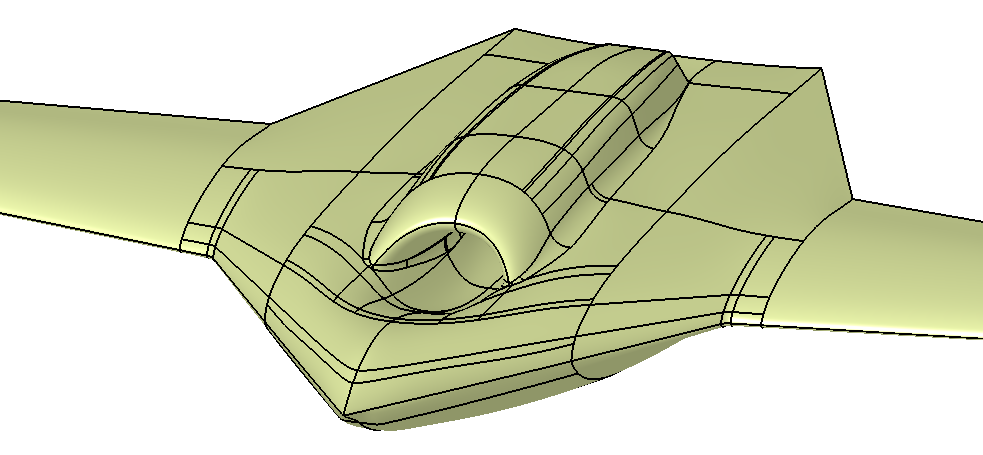
\includegraphics[width=0.8\textwidth]{BPS_Catia}
\caption{Компоновочная схема БПЛА-ЦАГИ}
\label{fig:BPS}
\end{figure}


%Выходим на основную проблему. Проблема интеграции двигателя и центроплана. Описанные выше требования приводят к проблемам. 

%Показываем наш БПЛА (модель из катьи), одним из решений является изогнутый центроплан.



\begin{figure}[ht]
\captionsetup{justification=centering}
\centering
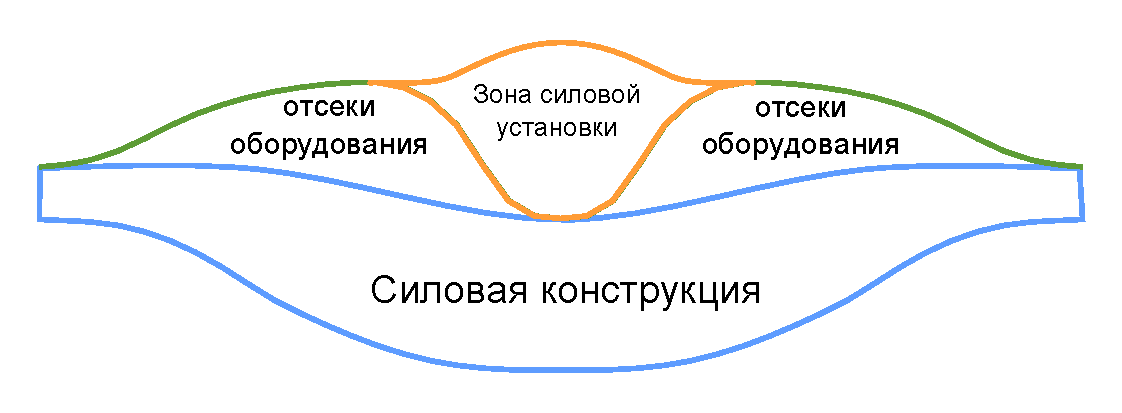
\includegraphics[width=\textwidth]{OriginalSectionWithEngine}
%%LaTeX with PSTricks extensions
%%Creator: inkscape 0.48.4
%%Please note this file requires PSTricks extensions
\psset{xunit=.5pt,yunit=.5pt,runit=.5pt}
\begin{pspicture}(1300,600)
{
\newrgbcolor{curcolor}{0.50196081 0.50196081 0.50196081}
\pscustom[linewidth=1,linecolor=curcolor,linestyle=dashed,dash=2 4]
{
\newpath
\moveto(94.3,127.2)
\lineto(1234.6,127.2)
\lineto(1234.61,127.2)
}
}
{
\newrgbcolor{curcolor}{0.50196081 0.50196081 0.50196081}
\pscustom[linewidth=1,linecolor=curcolor]
{
\newpath
\moveto(94.3,127.2)
\lineto(103.3,127.2)
\moveto(1234.6,127.2)
\lineto(1225.6,127.2)
\lineto(1225.61,127.2)
}
}
{
\newrgbcolor{curcolor}{0.50196081 0.50196081 0.50196081}
\pscustom[linestyle=none,fillstyle=solid,fillcolor=curcolor]
{
\newpath
\moveto(73.30712891,126.0984375)
\lineto(73.30712891,127.2703125)
\lineto(76.96923828,127.2703125)
\lineto(76.96923828,126.0984375)
\lineto(73.30712891,126.0984375)
}
}
{
\newrgbcolor{curcolor}{0.50196081 0.50196081 0.50196081}
\pscustom[linestyle=none,fillstyle=solid,fillcolor=curcolor]
{
\newpath
\moveto(78.79296875,122.7)
\lineto(78.79296875,123.82060547)
\lineto(81.42236328,123.82060547)
\lineto(81.42236328,131.76005859)
\lineto(79.09326172,130.09746094)
\lineto(79.09326172,131.34257812)
\lineto(81.53222656,133.01982422)
\lineto(82.74804688,133.01982422)
\lineto(82.74804688,123.82060547)
\lineto(85.26025391,123.82060547)
\lineto(85.26025391,122.7)
\lineto(78.79296875,122.7)
}
}
{
\newrgbcolor{curcolor}{0.50196081 0.50196081 0.50196081}
\pscustom[linewidth=1,linecolor=curcolor,linestyle=dashed,dash=2 4]
{
\newpath
\moveto(94.3,241.2)
\lineto(1234.6,241.2)
\lineto(1234.61,241.2)
}
}
{
\newrgbcolor{curcolor}{0.50196081 0.50196081 0.50196081}
\pscustom[linewidth=1,linecolor=curcolor]
{
\newpath
\moveto(94.3,241.2)
\lineto(103.3,241.2)
\moveto(1234.6,241.2)
\lineto(1225.6,241.2)
\lineto(1225.61,241.2)
}
}
{
\newrgbcolor{curcolor}{0.50196081 0.50196081 0.50196081}
\pscustom[linestyle=none,fillstyle=solid,fillcolor=curcolor]
{
\newpath
\moveto(60.79736328,240.0984375)
\lineto(60.79736328,241.2703125)
\lineto(64.45947266,241.2703125)
\lineto(64.45947266,240.0984375)
\lineto(60.79736328,240.0984375)
}
}
{
\newrgbcolor{curcolor}{0.50196081 0.50196081 0.50196081}
\pscustom[linestyle=none,fillstyle=solid,fillcolor=curcolor]
{
\newpath
\moveto(72.89697266,241.86357422)
\curveto(72.8969649,240.87235911)(72.80175015,240.03739901)(72.61132812,239.35869141)
\curveto(72.42577396,238.6848613)(72.16942656,238.13798684)(71.84228516,237.71806641)
\curveto(71.52001315,237.30302674)(71.13915416,237.00517548)(70.69970703,236.82451172)
\curveto(70.26024879,236.64384771)(69.79149926,236.55351577)(69.29345703,236.55351562)
\curveto(68.79052369,236.55351577)(68.32177416,236.64384771)(67.88720703,236.82451172)
\curveto(67.45263441,237.00517548)(67.07421682,237.30302674)(66.75195312,237.71806641)
\curveto(66.43456902,238.13310404)(66.18310443,238.67753708)(65.99755859,239.35136719)
\curveto(65.81689385,240.03007479)(65.72656191,240.8674763)(65.7265625,241.86357422)
\curveto(65.72656191,242.90360708)(65.81689385,243.76298122)(65.99755859,244.44169922)
\curveto(66.18310443,245.12528454)(66.43701042,245.66971759)(66.75927734,246.075)
\curveto(67.08154103,246.48026366)(67.46240002,246.7634665)(67.90185547,246.92460937)
\curveto(68.34130539,247.09061461)(68.81982054,247.17362234)(69.33740234,247.17363281)
\curveto(69.83056172,247.17362234)(70.29198704,247.09061461)(70.72167969,246.92460937)
\curveto(71.15624398,246.7634665)(71.53466157,246.48026366)(71.85693359,246.075)
\curveto(72.17919218,245.66971759)(72.43309818,245.12528454)(72.61865234,244.44169922)
\curveto(72.80419156,243.76298122)(72.8969649,242.90360708)(72.89697266,241.86357422)
\moveto(71.55664062,241.86357422)
\curveto(71.55663421,242.68388073)(71.50780613,243.3650324)(71.41015625,243.90703125)
\curveto(71.31249383,244.4538985)(71.168451,244.88846837)(70.97802734,245.21074219)
\curveto(70.78759201,245.53788179)(70.55321724,245.76737375)(70.27490234,245.89921875)
\curveto(70.00145998,246.03592816)(69.6889603,246.10428747)(69.33740234,246.10429687)
\curveto(68.96630477,246.10428747)(68.63915666,246.03592816)(68.35595703,245.89921875)
\curveto(68.07275097,245.76249094)(67.8334934,245.53055758)(67.63818359,245.20341797)
\curveto(67.4477516,244.88114416)(67.30370877,244.44657428)(67.20605469,243.89970703)
\curveto(67.10839647,243.35770819)(67.05956839,242.67899793)(67.05957031,241.86357422)
\curveto(67.05956839,241.07255422)(67.10839647,240.40605098)(67.20605469,239.8640625)
\curveto(67.30859158,239.32206769)(67.45507581,238.88505641)(67.64550781,238.55302734)
\curveto(67.84081761,238.22587738)(68.07763378,237.98906121)(68.35595703,237.84257812)
\curveto(68.63427385,237.70097556)(68.95165635,237.63017485)(69.30810547,237.63017578)
\curveto(69.65478064,237.63017485)(69.96728033,237.70097556)(70.24560547,237.84257812)
\curveto(70.5239204,237.98906121)(70.75829516,238.22587738)(70.94873047,238.55302734)
\curveto(71.14403697,238.88505641)(71.2929626,239.32206769)(71.39550781,239.8640625)
\curveto(71.50292333,240.40605098)(71.55663421,241.07255422)(71.55664062,241.86357422)
}
}
{
\newrgbcolor{curcolor}{0.50196081 0.50196081 0.50196081}
\pscustom[linestyle=none,fillstyle=solid,fillcolor=curcolor]
{
\newpath
\moveto(74.85986328,236.7)
\lineto(74.85986328,238.30400391)
\lineto(76.28808594,238.30400391)
\lineto(76.28808594,236.7)
\lineto(74.85986328,236.7)
}
}
{
\newrgbcolor{curcolor}{0.50196081 0.50196081 0.50196081}
\pscustom[linestyle=none,fillstyle=solid,fillcolor=curcolor]
{
\newpath
\moveto(85.36279297,240.06181641)
\curveto(85.36278526,239.54423544)(85.28466033,239.0706031)(85.12841797,238.64091797)
\curveto(84.97216065,238.21122896)(84.74022729,237.84013558)(84.43261719,237.52763672)
\curveto(84.12499353,237.22001901)(83.74169313,236.98076144)(83.28271484,236.80986328)
\curveto(82.8286081,236.6389649)(82.30126488,236.55351577)(81.70068359,236.55351562)
\curveto(81.1586879,236.55351577)(80.68505556,236.61699227)(80.27978516,236.74394531)
\curveto(79.8793923,236.87089827)(79.54003717,237.04423794)(79.26171875,237.26396484)
\curveto(78.9833971,237.48857343)(78.76122936,237.74980364)(78.59521484,238.04765625)
\curveto(78.43408125,238.34550617)(78.31933527,238.66533007)(78.25097656,239.00712891)
\lineto(79.58398438,239.1609375)
\curveto(79.63769333,238.96562273)(79.71337684,238.77519324)(79.81103516,238.58964844)
\curveto(79.90868915,238.40898267)(80.04052495,238.24540861)(80.20654297,238.09892578)
\curveto(80.37743868,237.95732296)(80.584958,237.84257698)(80.82910156,237.7546875)
\curveto(81.07812157,237.67167872)(81.37841424,237.63017485)(81.72998047,237.63017578)
\curveto(82.07177292,237.63017485)(82.38183121,237.68144433)(82.66015625,237.78398437)
\curveto(82.93847127,237.89140506)(83.17528744,238.0476549)(83.37060547,238.25273437)
\curveto(83.57079486,238.45781074)(83.7246033,238.70927533)(83.83203125,239.00712891)
\curveto(83.93944684,239.30497786)(83.99315772,239.6467744)(83.99316406,240.03251953)
\curveto(83.99315772,240.34989869)(83.94188824,240.64042575)(83.83935547,240.90410156)
\curveto(83.73681032,241.17265178)(83.59032609,241.40214374)(83.39990234,241.59257812)
\curveto(83.2094671,241.78788554)(82.97509233,241.93925257)(82.69677734,242.04667969)
\curveto(82.42333507,242.15409611)(82.11083538,242.20780699)(81.75927734,242.2078125)
\curveto(81.53954689,242.20780699)(81.33691038,242.18827576)(81.15136719,242.14921875)
\curveto(80.965817,242.11015084)(80.79247733,242.05643996)(80.63134766,241.98808594)
\curveto(80.47509483,241.91972134)(80.33105201,241.83915502)(80.19921875,241.74638672)
\curveto(80.0722632,241.65849114)(79.95263442,241.56571779)(79.84033203,241.46806641)
\lineto(78.55126953,241.46806641)
\lineto(78.89550781,247.01982422)
\lineto(84.76220703,247.01982422)
\lineto(84.76220703,245.89921875)
\lineto(80.09667969,245.89921875)
\lineto(79.89892578,242.62529297)
\curveto(80.1332983,242.80595093)(80.42626676,242.95975937)(80.77783203,243.08671875)
\curveto(81.12939105,243.21854817)(81.5468711,243.28446607)(82.03027344,243.28447266)
\curveto(82.54296386,243.28446607)(83.00438918,243.20634115)(83.41455078,243.05009766)
\curveto(83.82470086,242.89384146)(84.1738216,242.67167372)(84.46191406,242.38359375)
\curveto(84.7499929,242.10038522)(84.97216065,241.7610301)(85.12841797,241.36552734)
\curveto(85.28466033,240.97001526)(85.36278526,240.53544538)(85.36279297,240.06181641)
}
}
{
\newrgbcolor{curcolor}{0.50196081 0.50196081 0.50196081}
\pscustom[linewidth=1,linecolor=curcolor,linestyle=dashed,dash=2 4]
{
\newpath
\moveto(94.3,355.3)
\lineto(1234.6,355.3)
\lineto(1234.61,355.3)
}
}
{
\newrgbcolor{curcolor}{0.50196081 0.50196081 0.50196081}
\pscustom[linewidth=1,linecolor=curcolor]
{
\newpath
\moveto(94.3,355.3)
\lineto(103.3,355.3)
\moveto(1234.6,355.3)
\lineto(1225.6,355.3)
\lineto(1225.61,355.3)
}
}
{
\newrgbcolor{curcolor}{0.50196081 0.50196081 0.50196081}
\pscustom[linestyle=none,fillstyle=solid,fillcolor=curcolor]
{
\newpath
\moveto(85.40673828,355.96357422)
\curveto(85.40673052,354.97235911)(85.31151578,354.13739901)(85.12109375,353.45869141)
\curveto(84.93553959,352.7848613)(84.67919219,352.23798684)(84.35205078,351.81806641)
\curveto(84.02977878,351.40302674)(83.64891978,351.10517548)(83.20947266,350.92451172)
\curveto(82.77001441,350.74384771)(82.30126488,350.65351577)(81.80322266,350.65351563)
\curveto(81.30028932,350.65351577)(80.83153979,350.74384771)(80.39697266,350.92451172)
\curveto(79.96240003,351.10517548)(79.58398244,351.40302674)(79.26171875,351.81806641)
\curveto(78.94433464,352.23310404)(78.69287005,352.77753708)(78.50732422,353.45136719)
\curveto(78.32665948,354.13007479)(78.23632754,354.9674763)(78.23632812,355.96357422)
\curveto(78.23632754,357.00360708)(78.32665948,357.86298122)(78.50732422,358.54169922)
\curveto(78.69287005,359.22528454)(78.94677605,359.76971759)(79.26904297,360.175)
\curveto(79.59130665,360.58026366)(79.97216565,360.8634665)(80.41162109,361.02460938)
\curveto(80.85107102,361.19061461)(81.32958616,361.27362234)(81.84716797,361.27363281)
\curveto(82.34032734,361.27362234)(82.80175266,361.19061461)(83.23144531,361.02460938)
\curveto(83.66600961,360.8634665)(84.0444272,360.58026366)(84.36669922,360.175)
\curveto(84.68895781,359.76971759)(84.9428638,359.22528454)(85.12841797,358.54169922)
\curveto(85.31395718,357.86298122)(85.40673052,357.00360708)(85.40673828,355.96357422)
\moveto(84.06640625,355.96357422)
\curveto(84.06639983,356.78388073)(84.01757176,357.4650324)(83.91992188,358.00703125)
\curveto(83.82225945,358.5538985)(83.67821663,358.98846837)(83.48779297,359.31074219)
\curveto(83.29735763,359.63788179)(83.06298287,359.86737375)(82.78466797,359.99921875)
\curveto(82.51122561,360.13592816)(82.19872592,360.20428747)(81.84716797,360.20429688)
\curveto(81.47607039,360.20428747)(81.14892228,360.13592816)(80.86572266,359.99921875)
\curveto(80.5825166,359.86249094)(80.34325903,359.63055758)(80.14794922,359.30341797)
\curveto(79.95751722,358.98114416)(79.8134744,358.54657428)(79.71582031,357.99970703)
\curveto(79.61816209,357.45770819)(79.56933402,356.77899793)(79.56933594,355.96357422)
\curveto(79.56933402,355.17255422)(79.61816209,354.50605098)(79.71582031,353.9640625)
\curveto(79.81835721,353.42206769)(79.96484144,352.98505641)(80.15527344,352.65302734)
\curveto(80.35058324,352.32587738)(80.58739941,352.08906121)(80.86572266,351.94257813)
\curveto(81.14403948,351.80097556)(81.46142197,351.73017485)(81.81787109,351.73017578)
\curveto(82.16454627,351.73017485)(82.47704595,351.80097556)(82.75537109,351.94257813)
\curveto(83.03368602,352.08906121)(83.26806079,352.32587738)(83.45849609,352.65302734)
\curveto(83.65380259,352.98505641)(83.80272822,353.42206769)(83.90527344,353.9640625)
\curveto(84.01268895,354.50605098)(84.06639983,355.17255422)(84.06640625,355.96357422)
}
}
{
\newrgbcolor{curcolor}{0.50196081 0.50196081 0.50196081}
\pscustom[linewidth=1,linecolor=curcolor,linestyle=dashed,dash=2 4]
{
\newpath
\moveto(94.3,469.3)
\lineto(1234.6,469.3)
\lineto(1234.61,469.3)
}
}
{
\newrgbcolor{curcolor}{0.50196081 0.50196081 0.50196081}
\pscustom[linewidth=1,linecolor=curcolor]
{
\newpath
\moveto(94.3,469.3)
\lineto(103.3,469.3)
\moveto(1234.6,469.3)
\lineto(1225.6,469.3)
\lineto(1225.61,469.3)
}
}
{
\newrgbcolor{curcolor}{0.50196081 0.50196081 0.50196081}
\pscustom[linestyle=none,fillstyle=solid,fillcolor=curcolor]
{
\newpath
\moveto(72.89697266,469.96357422)
\curveto(72.8969649,468.97235911)(72.80175015,468.13739901)(72.61132812,467.45869141)
\curveto(72.42577396,466.7848613)(72.16942656,466.23798684)(71.84228516,465.81806641)
\curveto(71.52001315,465.40302674)(71.13915416,465.10517548)(70.69970703,464.92451172)
\curveto(70.26024879,464.74384771)(69.79149926,464.65351577)(69.29345703,464.65351563)
\curveto(68.79052369,464.65351577)(68.32177416,464.74384771)(67.88720703,464.92451172)
\curveto(67.45263441,465.10517548)(67.07421682,465.40302674)(66.75195312,465.81806641)
\curveto(66.43456902,466.23310404)(66.18310443,466.77753708)(65.99755859,467.45136719)
\curveto(65.81689385,468.13007479)(65.72656191,468.9674763)(65.7265625,469.96357422)
\curveto(65.72656191,471.00360708)(65.81689385,471.86298122)(65.99755859,472.54169922)
\curveto(66.18310443,473.22528454)(66.43701042,473.76971759)(66.75927734,474.175)
\curveto(67.08154103,474.58026366)(67.46240002,474.8634665)(67.90185547,475.02460938)
\curveto(68.34130539,475.19061461)(68.81982054,475.27362234)(69.33740234,475.27363281)
\curveto(69.83056172,475.27362234)(70.29198704,475.19061461)(70.72167969,475.02460938)
\curveto(71.15624398,474.8634665)(71.53466157,474.58026366)(71.85693359,474.175)
\curveto(72.17919218,473.76971759)(72.43309818,473.22528454)(72.61865234,472.54169922)
\curveto(72.80419156,471.86298122)(72.8969649,471.00360708)(72.89697266,469.96357422)
\moveto(71.55664062,469.96357422)
\curveto(71.55663421,470.78388073)(71.50780613,471.4650324)(71.41015625,472.00703125)
\curveto(71.31249383,472.5538985)(71.168451,472.98846837)(70.97802734,473.31074219)
\curveto(70.78759201,473.63788179)(70.55321724,473.86737375)(70.27490234,473.99921875)
\curveto(70.00145998,474.13592816)(69.6889603,474.20428747)(69.33740234,474.20429688)
\curveto(68.96630477,474.20428747)(68.63915666,474.13592816)(68.35595703,473.99921875)
\curveto(68.07275097,473.86249094)(67.8334934,473.63055758)(67.63818359,473.30341797)
\curveto(67.4477516,472.98114416)(67.30370877,472.54657428)(67.20605469,471.99970703)
\curveto(67.10839647,471.45770819)(67.05956839,470.77899793)(67.05957031,469.96357422)
\curveto(67.05956839,469.17255422)(67.10839647,468.50605098)(67.20605469,467.9640625)
\curveto(67.30859158,467.42206769)(67.45507581,466.98505641)(67.64550781,466.65302734)
\curveto(67.84081761,466.32587738)(68.07763378,466.08906121)(68.35595703,465.94257813)
\curveto(68.63427385,465.80097556)(68.95165635,465.73017485)(69.30810547,465.73017578)
\curveto(69.65478064,465.73017485)(69.96728033,465.80097556)(70.24560547,465.94257813)
\curveto(70.5239204,466.08906121)(70.75829516,466.32587738)(70.94873047,466.65302734)
\curveto(71.14403697,466.98505641)(71.2929626,467.42206769)(71.39550781,467.9640625)
\curveto(71.50292333,468.50605098)(71.55663421,469.17255422)(71.55664062,469.96357422)
}
}
{
\newrgbcolor{curcolor}{0.50196081 0.50196081 0.50196081}
\pscustom[linestyle=none,fillstyle=solid,fillcolor=curcolor]
{
\newpath
\moveto(74.85986328,464.8)
\lineto(74.85986328,466.40400391)
\lineto(76.28808594,466.40400391)
\lineto(76.28808594,464.8)
\lineto(74.85986328,464.8)
}
}
{
\newrgbcolor{curcolor}{0.50196081 0.50196081 0.50196081}
\pscustom[linestyle=none,fillstyle=solid,fillcolor=curcolor]
{
\newpath
\moveto(85.36279297,468.16181641)
\curveto(85.36278526,467.64423544)(85.28466033,467.1706031)(85.12841797,466.74091797)
\curveto(84.97216065,466.31122896)(84.74022729,465.94013558)(84.43261719,465.62763672)
\curveto(84.12499353,465.32001901)(83.74169313,465.08076144)(83.28271484,464.90986328)
\curveto(82.8286081,464.7389649)(82.30126488,464.65351577)(81.70068359,464.65351563)
\curveto(81.1586879,464.65351577)(80.68505556,464.71699227)(80.27978516,464.84394531)
\curveto(79.8793923,464.97089827)(79.54003717,465.14423794)(79.26171875,465.36396484)
\curveto(78.9833971,465.58857343)(78.76122936,465.84980364)(78.59521484,466.14765625)
\curveto(78.43408125,466.44550617)(78.31933527,466.76533007)(78.25097656,467.10712891)
\lineto(79.58398438,467.2609375)
\curveto(79.63769333,467.06562273)(79.71337684,466.87519324)(79.81103516,466.68964844)
\curveto(79.90868915,466.50898267)(80.04052495,466.34540861)(80.20654297,466.19892578)
\curveto(80.37743868,466.05732296)(80.584958,465.94257698)(80.82910156,465.8546875)
\curveto(81.07812157,465.77167872)(81.37841424,465.73017485)(81.72998047,465.73017578)
\curveto(82.07177292,465.73017485)(82.38183121,465.78144433)(82.66015625,465.88398438)
\curveto(82.93847127,465.99140506)(83.17528744,466.1476549)(83.37060547,466.35273438)
\curveto(83.57079486,466.55781074)(83.7246033,466.80927533)(83.83203125,467.10712891)
\curveto(83.93944684,467.40497786)(83.99315772,467.7467744)(83.99316406,468.13251953)
\curveto(83.99315772,468.44989869)(83.94188824,468.74042575)(83.83935547,469.00410156)
\curveto(83.73681032,469.27265178)(83.59032609,469.50214374)(83.39990234,469.69257813)
\curveto(83.2094671,469.88788554)(82.97509233,470.03925257)(82.69677734,470.14667969)
\curveto(82.42333507,470.25409611)(82.11083538,470.30780699)(81.75927734,470.3078125)
\curveto(81.53954689,470.30780699)(81.33691038,470.28827576)(81.15136719,470.24921875)
\curveto(80.965817,470.21015084)(80.79247733,470.15643996)(80.63134766,470.08808594)
\curveto(80.47509483,470.01972134)(80.33105201,469.93915502)(80.19921875,469.84638672)
\curveto(80.0722632,469.75849114)(79.95263442,469.66571779)(79.84033203,469.56806641)
\lineto(78.55126953,469.56806641)
\lineto(78.89550781,475.11982422)
\lineto(84.76220703,475.11982422)
\lineto(84.76220703,473.99921875)
\lineto(80.09667969,473.99921875)
\lineto(79.89892578,470.72529297)
\curveto(80.1332983,470.90595093)(80.42626676,471.05975937)(80.77783203,471.18671875)
\curveto(81.12939105,471.31854817)(81.5468711,471.38446607)(82.03027344,471.38447266)
\curveto(82.54296386,471.38446607)(83.00438918,471.30634115)(83.41455078,471.15009766)
\curveto(83.82470086,470.99384146)(84.1738216,470.77167372)(84.46191406,470.48359375)
\curveto(84.7499929,470.20038522)(84.97216065,469.8610301)(85.12841797,469.46552734)
\curveto(85.28466033,469.07001526)(85.36278526,468.63544538)(85.36279297,468.16181641)
}
}
{
\newrgbcolor{curcolor}{0.50196081 0.50196081 0.50196081}
\pscustom[linewidth=1,linecolor=curcolor,linestyle=dashed,dash=2 4]
{
\newpath
\moveto(94.3,583.3)
\lineto(1234.6,583.3)
\lineto(1234.61,583.3)
}
}
{
\newrgbcolor{curcolor}{0.50196081 0.50196081 0.50196081}
\pscustom[linewidth=1,linecolor=curcolor]
{
\newpath
\moveto(94.3,583.3)
\lineto(103.3,583.3)
\moveto(1234.6,583.3)
\lineto(1225.6,583.3)
\lineto(1225.61,583.3)
}
}
{
\newrgbcolor{curcolor}{0.50196081 0.50196081 0.50196081}
\pscustom[linestyle=none,fillstyle=solid,fillcolor=curcolor]
{
\newpath
\moveto(78.79296875,578.8)
\lineto(78.79296875,579.92060547)
\lineto(81.42236328,579.92060547)
\lineto(81.42236328,587.86005859)
\lineto(79.09326172,586.19746094)
\lineto(79.09326172,587.44257812)
\lineto(81.53222656,589.11982422)
\lineto(82.74804688,589.11982422)
\lineto(82.74804688,579.92060547)
\lineto(85.26025391,579.92060547)
\lineto(85.26025391,578.8)
\lineto(78.79296875,578.8)
}
}
{
\newrgbcolor{curcolor}{0.50196081 0.50196081 0.50196081}
\pscustom[linewidth=1,linecolor=curcolor,linestyle=dashed,dash=2 4]
{
\newpath
\moveto(208.3,36)
\lineto(208.3,583.3)
\lineto(208.31,583.3)
}
}
{
\newrgbcolor{curcolor}{0.50196081 0.50196081 0.50196081}
\pscustom[linewidth=1,linecolor=curcolor]
{
\newpath
\moveto(208.3,36)
\lineto(208.3,45)
\moveto(208.3,583.3)
\lineto(208.3,574.3)
\lineto(208.31,574.3)
}
}
{
\newrgbcolor{curcolor}{0.50196081 0.50196081 0.50196081}
\pscustom[linestyle=none,fillstyle=solid,fillcolor=curcolor]
{
\newpath
\moveto(202.28681641,16.8984375)
\lineto(202.28681641,18.0703125)
\lineto(205.94892578,18.0703125)
\lineto(205.94892578,16.8984375)
\lineto(202.28681641,16.8984375)
}
}
{
\newrgbcolor{curcolor}{0.50196081 0.50196081 0.50196081}
\pscustom[linestyle=none,fillstyle=solid,fillcolor=curcolor]
{
\newpath
\moveto(207.38447266,13.5)
\lineto(207.38447266,14.43017578)
\curveto(207.63349509,15.00146334)(207.93622916,15.50439253)(208.29267578,15.93896484)
\curveto(208.65400188,16.37841509)(209.03241947,16.77392251)(209.42792969,17.12548828)
\curveto(209.82343431,17.48192961)(210.21405892,17.81151913)(210.59980469,18.11425781)
\curveto(210.99042533,18.41698727)(211.34198748,18.71972134)(211.65449219,19.02246094)
\curveto(211.96698685,19.32518949)(212.21845144,19.64257198)(212.40888672,19.97460938)
\curveto(212.60419324,20.30663382)(212.7018494,20.68261)(212.70185547,21.10253906)
\curveto(212.7018494,21.39549992)(212.65790413,21.65184732)(212.57001953,21.87158203)
\curveto(212.48212305,22.09618281)(212.35517006,22.2841709)(212.18916016,22.43554688)
\curveto(212.02313914,22.58690498)(211.82294403,22.69920955)(211.58857422,22.77246094)
\curveto(211.3590773,22.85057659)(211.1027299,22.88963905)(210.81953125,22.88964844)
\curveto(210.55585545,22.88963905)(210.30683226,22.85301799)(210.07246094,22.77978516)
\curveto(209.84296554,22.70653376)(209.63788762,22.59667059)(209.45722656,22.45019531)
\curveto(209.27655985,22.30370213)(209.12763422,22.12059685)(209.01044922,21.90087891)
\curveto(208.89814226,21.68602697)(208.82490015,21.43456238)(208.79072266,21.14648438)
\lineto(207.44306641,21.27099609)
\curveto(207.48701086,21.6420817)(207.58954982,21.99120245)(207.75068359,22.31835938)
\curveto(207.91181512,22.64549867)(208.13398287,22.93114291)(208.4171875,23.17529297)
\curveto(208.70038855,23.42430648)(209.03974368,23.61961879)(209.43525391,23.76123047)
\curveto(209.83564133,23.90282163)(210.29706665,23.97362234)(210.81953125,23.97363281)
\curveto(211.33222186,23.97362234)(211.78876437,23.91258724)(212.18916016,23.79052734)
\curveto(212.58954482,23.66844686)(212.92645855,23.48778298)(213.19990234,23.24853516)
\curveto(213.47821581,23.00926783)(213.69061794,22.71385797)(213.83710938,22.36230469)
\curveto(213.9835864,22.01073368)(214.05682851,21.60546064)(214.05683594,21.14648438)
\curveto(214.05682851,20.79979739)(213.99335201,20.47020787)(213.86640625,20.15771484)
\curveto(213.74432882,19.8452085)(213.57831336,19.54735723)(213.36835938,19.26416016)
\curveto(213.16327472,18.98095155)(212.92401714,18.70751432)(212.65058594,18.44384766)
\curveto(212.37714269,18.1801711)(212.09149844,17.9213823)(211.79365234,17.66748047)
\curveto(211.49579592,17.41845311)(211.19550325,17.16942992)(210.89277344,16.92041016)
\curveto(210.5900351,16.67626635)(210.30439086,16.42968457)(210.03583984,16.18066406)
\curveto(209.77216483,15.93163819)(209.53534866,15.6777322)(209.32539063,15.41894531)
\curveto(209.1154272,15.1650374)(208.95185315,14.89892438)(208.83466797,14.62060547)
\lineto(214.21796875,14.62060547)
\lineto(214.21796875,13.5)
\lineto(207.38447266,13.5)
}
}
{
\newrgbcolor{curcolor}{0.50196081 0.50196081 0.50196081}
\pscustom[linewidth=1,linecolor=curcolor,linestyle=dashed,dash=2 4]
{
\newpath
\moveto(436.4,36)
\lineto(436.4,583.3)
\lineto(436.41,583.3)
}
}
{
\newrgbcolor{curcolor}{0.50196081 0.50196081 0.50196081}
\pscustom[linewidth=1,linecolor=curcolor]
{
\newpath
\moveto(436.4,36)
\lineto(436.4,45)
\moveto(436.4,583.3)
\lineto(436.4,574.3)
\lineto(436.41,574.3)
}
}
{
\newrgbcolor{curcolor}{0.50196081 0.50196081 0.50196081}
\pscustom[linestyle=none,fillstyle=solid,fillcolor=curcolor]
{
\newpath
\moveto(430.38681641,16.8984375)
\lineto(430.38681641,18.0703125)
\lineto(434.04892578,18.0703125)
\lineto(434.04892578,16.8984375)
\lineto(430.38681641,16.8984375)
}
}
{
\newrgbcolor{curcolor}{0.50196081 0.50196081 0.50196081}
\pscustom[linestyle=none,fillstyle=solid,fillcolor=curcolor]
{
\newpath
\moveto(435.87265625,13.5)
\lineto(435.87265625,14.62060547)
\lineto(438.50205078,14.62060547)
\lineto(438.50205078,22.56005859)
\lineto(436.17294922,20.89746094)
\lineto(436.17294922,22.14257812)
\lineto(438.61191406,23.81982422)
\lineto(439.82773437,23.81982422)
\lineto(439.82773437,14.62060547)
\lineto(442.33994141,14.62060547)
\lineto(442.33994141,13.5)
\lineto(435.87265625,13.5)
}
}
{
\newrgbcolor{curcolor}{0.50196081 0.50196081 0.50196081}
\pscustom[linewidth=1,linecolor=curcolor,linestyle=dashed,dash=2 4]
{
\newpath
\moveto(664.5,36)
\lineto(664.5,583.3)
\lineto(664.51,583.3)
}
}
{
\newrgbcolor{curcolor}{0.50196081 0.50196081 0.50196081}
\pscustom[linewidth=1,linecolor=curcolor]
{
\newpath
\moveto(664.5,36)
\lineto(664.5,45)
\moveto(664.5,583.3)
\lineto(664.5,574.3)
\lineto(664.51,574.3)
}
}
{
\newrgbcolor{curcolor}{0.50196081 0.50196081 0.50196081}
\pscustom[linestyle=none,fillstyle=solid,fillcolor=curcolor]
{
\newpath
\moveto(668.08154297,18.66357422)
\curveto(668.08153521,17.67235911)(667.98632046,16.83739901)(667.79589844,16.15869141)
\curveto(667.61034428,15.4848613)(667.35399688,14.93798684)(667.02685547,14.51806641)
\curveto(666.70458346,14.10302674)(666.32372447,13.80517548)(665.88427734,13.62451172)
\curveto(665.4448191,13.44384771)(664.97606957,13.35351577)(664.47802734,13.35351562)
\curveto(663.97509401,13.35351577)(663.50634448,13.44384771)(663.07177734,13.62451172)
\curveto(662.63720472,13.80517548)(662.25878713,14.10302674)(661.93652344,14.51806641)
\curveto(661.61913933,14.93310404)(661.36767474,15.47753708)(661.18212891,16.15136719)
\curveto(661.00146417,16.83007479)(660.91113223,17.6674763)(660.91113281,18.66357422)
\curveto(660.91113223,19.70360708)(661.00146417,20.56298122)(661.18212891,21.24169922)
\curveto(661.36767474,21.92528454)(661.62158073,22.46971759)(661.94384766,22.875)
\curveto(662.26611134,23.28026366)(662.64697033,23.5634665)(663.08642578,23.72460938)
\curveto(663.52587571,23.89061461)(664.00439085,23.97362234)(664.52197266,23.97363281)
\curveto(665.01513203,23.97362234)(665.47655735,23.89061461)(665.90625,23.72460938)
\curveto(666.3408143,23.5634665)(666.71923189,23.28026366)(667.04150391,22.875)
\curveto(667.36376249,22.46971759)(667.61766849,21.92528454)(667.80322266,21.24169922)
\curveto(667.98876187,20.56298122)(668.08153521,19.70360708)(668.08154297,18.66357422)
\moveto(666.74121094,18.66357422)
\curveto(666.74120452,19.48388073)(666.69237645,20.1650324)(666.59472656,20.70703125)
\curveto(666.49706414,21.2538985)(666.35302132,21.68846837)(666.16259766,22.01074219)
\curveto(665.97216232,22.33788179)(665.73778756,22.56737375)(665.45947266,22.69921875)
\curveto(665.1860303,22.83592816)(664.87353061,22.90428747)(664.52197266,22.90429688)
\curveto(664.15087508,22.90428747)(663.82372697,22.83592816)(663.54052734,22.69921875)
\curveto(663.25732129,22.56249094)(663.01806371,22.33055758)(662.82275391,22.00341797)
\curveto(662.63232191,21.68114416)(662.48827909,21.24657428)(662.390625,20.69970703)
\curveto(662.29296678,20.15770819)(662.24413871,19.47899793)(662.24414062,18.66357422)
\curveto(662.24413871,17.87255422)(662.29296678,17.20605098)(662.390625,16.6640625)
\curveto(662.49316189,16.12206769)(662.63964612,15.68505641)(662.83007812,15.35302734)
\curveto(663.02538792,15.02587738)(663.26220409,14.78906121)(663.54052734,14.64257812)
\curveto(663.81884416,14.50097556)(664.13622666,14.43017485)(664.49267578,14.43017578)
\curveto(664.83935095,14.43017485)(665.15185064,14.50097556)(665.43017578,14.64257812)
\curveto(665.70849071,14.78906121)(665.94286548,15.02587738)(666.13330078,15.35302734)
\curveto(666.32860728,15.68505641)(666.47753291,16.12206769)(666.58007812,16.6640625)
\curveto(666.68749364,17.20605098)(666.74120452,17.87255422)(666.74121094,18.66357422)
}
}
{
\newrgbcolor{curcolor}{0.50196081 0.50196081 0.50196081}
\pscustom[linewidth=1,linecolor=curcolor,linestyle=dashed,dash=2 4]
{
\newpath
\moveto(892.5,36)
\lineto(892.5,583.3)
\lineto(892.51,583.3)
}
}
{
\newrgbcolor{curcolor}{0.50196081 0.50196081 0.50196081}
\pscustom[linewidth=1,linecolor=curcolor]
{
\newpath
\moveto(892.5,36)
\lineto(892.5,45)
\moveto(892.5,583.3)
\lineto(892.5,574.3)
\lineto(892.51,574.3)
}
}
{
\newrgbcolor{curcolor}{0.50196081 0.50196081 0.50196081}
\pscustom[linestyle=none,fillstyle=solid,fillcolor=curcolor]
{
\newpath
\moveto(889.46777344,13.5)
\lineto(889.46777344,14.62060547)
\lineto(892.09716797,14.62060547)
\lineto(892.09716797,22.56005859)
\lineto(889.76806641,20.89746094)
\lineto(889.76806641,22.14257812)
\lineto(892.20703125,23.81982422)
\lineto(893.42285156,23.81982422)
\lineto(893.42285156,14.62060547)
\lineto(895.93505859,14.62060547)
\lineto(895.93505859,13.5)
\lineto(889.46777344,13.5)
}
}
{
\newrgbcolor{curcolor}{0.50196081 0.50196081 0.50196081}
\pscustom[linewidth=1,linecolor=curcolor,linestyle=dashed,dash=2 4]
{
\newpath
\moveto(1120.6,36)
\lineto(1120.6,538.3)
\moveto(1120.6,574.3)
\lineto(1120.6,583.3)
\lineto(1120.61,583.3)
}
}
{
\newrgbcolor{curcolor}{0.50196081 0.50196081 0.50196081}
\pscustom[linewidth=1,linecolor=curcolor]
{
\newpath
\moveto(1120.6,36)
\lineto(1120.6,45)
\moveto(1120.6,583.3)
\lineto(1120.6,574.3)
\lineto(1120.61,574.3)
}
}
{
\newrgbcolor{curcolor}{0.50196081 0.50196081 0.50196081}
\pscustom[linestyle=none,fillstyle=solid,fillcolor=curcolor]
{
\newpath
\moveto(1117.17958984,13.5)
\lineto(1117.17958984,14.43017578)
\curveto(1117.42861228,15.00146334)(1117.73134635,15.50439253)(1118.08779297,15.93896484)
\curveto(1118.44911907,16.37841509)(1118.82753666,16.77392251)(1119.22304687,17.12548828)
\curveto(1119.61855149,17.48192961)(1120.0091761,17.81151913)(1120.39492187,18.11425781)
\curveto(1120.78554251,18.41698727)(1121.13710466,18.71972134)(1121.44960937,19.02246094)
\curveto(1121.76210404,19.32518949)(1122.01356863,19.64257198)(1122.20400391,19.97460938)
\curveto(1122.39931043,20.30663382)(1122.49696658,20.68261)(1122.49697266,21.10253906)
\curveto(1122.49696658,21.39549992)(1122.45302132,21.65184732)(1122.36513672,21.87158203)
\curveto(1122.27724024,22.09618281)(1122.15028724,22.2841709)(1121.98427734,22.43554688)
\curveto(1121.81825633,22.58690498)(1121.61806121,22.69920955)(1121.38369141,22.77246094)
\curveto(1121.15419449,22.85057659)(1120.89784709,22.88963905)(1120.61464844,22.88964844)
\curveto(1120.35097264,22.88963905)(1120.10194945,22.85301799)(1119.86757812,22.77978516)
\curveto(1119.63808272,22.70653376)(1119.4330048,22.59667059)(1119.25234375,22.45019531)
\curveto(1119.07167704,22.30370213)(1118.92275141,22.12059685)(1118.80556641,21.90087891)
\curveto(1118.69325945,21.68602697)(1118.62001734,21.43456238)(1118.58583984,21.14648438)
\lineto(1117.23818359,21.27099609)
\curveto(1117.28212805,21.6420817)(1117.38466701,21.99120245)(1117.54580078,22.31835938)
\curveto(1117.70693231,22.64549867)(1117.92910006,22.93114291)(1118.21230469,23.17529297)
\curveto(1118.49550574,23.42430648)(1118.83486087,23.61961879)(1119.23037109,23.76123047)
\curveto(1119.63075851,23.90282163)(1120.09218383,23.97362234)(1120.61464844,23.97363281)
\curveto(1121.12733905,23.97362234)(1121.58388156,23.91258724)(1121.98427734,23.79052734)
\curveto(1122.38466201,23.66844686)(1122.72157573,23.48778298)(1122.99501953,23.24853516)
\curveto(1123.273333,23.00926783)(1123.48573513,22.71385797)(1123.63222656,22.36230469)
\curveto(1123.77870358,22.01073368)(1123.8519457,21.60546064)(1123.85195312,21.14648438)
\curveto(1123.8519457,20.79979739)(1123.7884692,20.47020787)(1123.66152344,20.15771484)
\curveto(1123.53944601,19.8452085)(1123.37343055,19.54735723)(1123.16347656,19.26416016)
\curveto(1122.9583919,18.98095155)(1122.71913433,18.70751432)(1122.44570312,18.44384766)
\curveto(1122.17225988,18.1801711)(1121.88661563,17.9213823)(1121.58876953,17.66748047)
\curveto(1121.2909131,17.41845311)(1120.99062043,17.16942992)(1120.68789062,16.92041016)
\curveto(1120.38515229,16.67626635)(1120.09950804,16.42968457)(1119.83095703,16.18066406)
\curveto(1119.56728201,15.93163819)(1119.33046584,15.6777322)(1119.12050781,15.41894531)
\curveto(1118.91054439,15.1650374)(1118.74697033,14.89892438)(1118.62978516,14.62060547)
\lineto(1124.01308594,14.62060547)
\lineto(1124.01308594,13.5)
\lineto(1117.17958984,13.5)
}
}
{
\newrgbcolor{curcolor}{0.50196081 0.50196081 0.50196081}
\pscustom[linewidth=1,linecolor=curcolor]
{
\newpath
\moveto(94.3,583.3)
\lineto(94.3,36)
\lineto(1234.6,36)
\moveto(1234.6,583.3)
\moveto(94.3,583.3)
\lineto(94.31,583.3)
}
}
{
\newrgbcolor{curcolor}{0.36862746 0.61176473 0.21176471}
\pscustom[linewidth=5,linecolor=curcolor]
{
\newpath
\moveto(105.7,355.3)
\lineto(106,355.3)
\lineto(106.8,355.3)
\lineto(108.5,355.3)
\lineto(111.3,355.3)
\lineto(116.9,354.9)
\lineto(122.5,354.7)
\lineto(133.6,354.3)
\lineto(147.6,353.6)
\lineto(161.6,352.7)
\lineto(189.5,349.2)
\lineto(217.5,342.6)
\lineto(245.4,332.9)
\lineto(273.3,320.1)
\lineto(301.3,304.3)
\lineto(329.2,286.5)
\lineto(357.1,269.2)
\lineto(385.1,255.1)
\lineto(413,242.3)
\lineto(441,230.5)
\lineto(468.9,220)
\lineto(496.8,211.2)
\lineto(524.8,204.2)
\lineto(552.7,199.3)
\lineto(580.6,196.2)
\lineto(608.6,194.6)
\lineto(636.5,194.2)
\lineto(664.5,194.2)
\lineto(692.4,194.2)
\lineto(720.3,194.6)
\lineto(748.3,196.2)
\lineto(776.2,199.3)
\lineto(804.1,204.2)
\lineto(832.1,211.2)
\lineto(860,220)
\lineto(887.9,230.5)
\lineto(915.9,242.3)
\lineto(943.8,255.1)
\lineto(971.8,269.2)
\lineto(999.7,286.5)
\lineto(1027.6,304.3)
\lineto(1055.6,320.1)
\lineto(1083.5,332.9)
\lineto(1111.4,342.6)
\lineto(1139.4,349.2)
\lineto(1167.3,352.7)
\lineto(1181.3,353.6)
\lineto(1195.3,354.3)
\lineto(1206.4,354.7)
\lineto(1212,354.9)
\lineto(1217.6,355.3)
\lineto(1220.4,355.3)
\lineto(1222.1,355.3)
\lineto(1222.9,355.3)
\lineto(1223.2,355.3)
\lineto(1223.21,355.3)
}
}
{
\newrgbcolor{curcolor}{0.36862746 0.61176473 0.21176471}
\pscustom[linewidth=5,linecolor=curcolor]
{
\newpath
\moveto(105.7,412)
\lineto(106,412)
\lineto(106.8,412)
\lineto(108.5,412.1)
\lineto(111.3,412.3)
\lineto(116.9,412.7)
\lineto(122.5,413.2)
\lineto(133.6,414.4)
\lineto(147.6,416.6)
\lineto(161.6,419.6)
\lineto(189.5,428.7)
\lineto(217.5,441.7)
\lineto(245.4,455.8)
\lineto(273.3,468.3)
\lineto(301.3,478.3)
\lineto(329.2,486.3)
\lineto(357.1,492.5)
\lineto(385.1,497)
\lineto(413,500.3)
\lineto(441,502.2)
\lineto(468.9,502.1)
\lineto(496.8,496.8)
\lineto(524.8,482.5)
\lineto(552.7,457)
\lineto(580.6,414.4)
\lineto(608.6,375.6)
\lineto(636.5,359.2)
\lineto(664.5,356.6)
\lineto(692.4,359.2)
\lineto(720.3,375.6)
\lineto(748.3,414.4)
\lineto(776.2,457)
\lineto(804.1,482.5)
\lineto(832.1,496.8)
\lineto(860,502.1)
\lineto(887.9,502.2)
\lineto(915.9,500.3)
\lineto(943.8,497)
\lineto(971.8,492.5)
\lineto(999.7,486.3)
\lineto(1027.6,478.3)
\lineto(1055.6,468.3)
\lineto(1083.5,455.8)
\lineto(1111.4,441.7)
\lineto(1139.4,428.7)
\lineto(1167.3,419.6)
\lineto(1181.3,416.6)
\lineto(1195.3,414.4)
\lineto(1206.4,413.2)
\lineto(1212,412.7)
\lineto(1217.6,412.3)
\lineto(1220.4,412.1)
\lineto(1222.1,412)
\lineto(1222.9,412)
\lineto(1223.2,412)
\lineto(1223.21,412)
}
}
{
\newrgbcolor{curcolor}{1 0.08627451 0.08627451}
\pscustom[linewidth=13.58276261,linecolor=curcolor]
{
\newpath
\moveto(740.44041571,452.849293)
\curveto(740.44041571,411.18471237)(706.66459963,377.40889629)(665.000019,377.40889629)
\curveto(623.33543837,377.40889629)(589.55962229,411.18471237)(589.55962229,452.849293)
\curveto(589.55962229,494.51387363)(623.33543837,528.28968971)(665.000019,528.28968971)
\curveto(706.66459963,528.28968971)(740.44041571,494.51387363)(740.44041571,452.849293)
\closepath
}
}
{
\newrgbcolor{curcolor}{0 0 0}
\pscustom[linestyle=none,fillstyle=solid,fillcolor=curcolor]
{
\newpath
\moveto(359.12109375,633.32031206)
\lineto(372.01171875,633.32031206)
\lineto(372.01171875,655.83984331)
\lineto(362.5390625,655.83984331)
\lineto(362.5390625,651.69921831)
\curveto(362.53904996,645.20180727)(361.80988402,639.79816684)(360.3515625,635.48828081)
\curveto(360.05207328,634.60285954)(359.64191744,633.88020401)(359.12109375,633.32031206)
\moveto(353.359375,633.32031206)
\curveto(355.10416156,634.14062042)(356.22395211,635.33202548)(356.71875,636.89453081)
\curveto(357.98176285,640.90493657)(358.61327264,646.49086848)(358.61328125,653.65234331)
\lineto(358.61328125,659.16015581)
\lineto(375.95703125,659.16015581)
\lineto(375.95703125,633.32031206)
\lineto(379.27734375,633.32031206)
\lineto(379.27734375,623.73046831)
\lineto(375.95703125,623.73046831)
\lineto(375.95703125,629.99999956)
\lineto(355.29296875,629.99999956)
\lineto(355.29296875,623.73046831)
\lineto(351.97265625,623.73046831)
\lineto(351.97265625,633.32031206)
\lineto(353.359375,633.32031206)
}
}
{
\newrgbcolor{curcolor}{0 0 0}
\pscustom[linestyle=none,fillstyle=solid,fillcolor=curcolor]
{
\newpath
\moveto(388.4765625,640.07812456)
\lineto(388.4765625,632.87109331)
\lineto(393.59375,632.87109331)
\curveto(395.23436102,632.87109044)(396.48435977,633.17707971)(397.34375,633.78906206)
\curveto(398.20310805,634.41405764)(398.63279512,635.31249424)(398.6328125,636.48437456)
\curveto(398.63279512,637.6562419)(398.20310805,638.54816809)(397.34375,639.16015581)
\curveto(396.48435977,639.7721252)(395.23436102,640.07811448)(393.59375,640.07812456)
\lineto(388.4765625,640.07812456)
\moveto(388.4765625,649.00390581)
\lineto(388.4765625,642.94921831)
\lineto(393.203125,642.94921831)
\curveto(394.55727836,642.94920536)(395.66404809,643.21613217)(396.5234375,643.74999956)
\curveto(397.38279637,644.29686026)(397.81248344,645.05206784)(397.8125,646.01562456)
\curveto(397.81248344,646.97914924)(397.38279637,647.71482559)(396.5234375,648.22265581)
\curveto(395.66404809,648.7434704)(394.55727836,649.0038868)(393.203125,649.00390581)
\lineto(388.4765625,649.00390581)
\moveto(384.8828125,651.87499956)
\lineto(393.4375,651.87499956)
\curveto(396.00258941,651.87497768)(397.97524369,651.40622815)(399.35546875,650.46874956)
\curveto(400.7356576,649.53123003)(401.42576107,648.19659594)(401.42578125,646.46484331)
\curveto(401.42576107,645.12368235)(401.07419893,644.05597508)(400.37109375,643.26171831)
\curveto(399.66795033,642.48045583)(398.62628471,641.99217506)(397.24609375,641.79687456)
\curveto(398.89972193,641.48436307)(400.18227273,640.83332206)(401.09375,639.84374956)
\curveto(402.00518758,638.85415737)(402.46091629,637.61717944)(402.4609375,636.13281206)
\curveto(402.46091629,634.17968288)(401.70570871,632.66926772)(400.1953125,631.60156206)
\curveto(398.69789922,630.53385319)(396.55597428,629.99999956)(393.76953125,629.99999956)
\lineto(384.8828125,629.99999956)
\lineto(384.8828125,651.87499956)
}
}
{
\newrgbcolor{curcolor}{0 0 0}
\pscustom[linestyle=none,fillstyle=solid,fillcolor=curcolor]
{
\newpath
\moveto(427.20703125,651.87499956)
\lineto(427.20703125,629.99999956)
\lineto(423.6328125,629.99999956)
\lineto(423.6328125,647.55859331)
\lineto(413.0859375,629.99999956)
\lineto(408.4765625,629.99999956)
\lineto(408.4765625,651.87499956)
\lineto(412.05078125,651.87499956)
\lineto(412.05078125,634.35546831)
\lineto(422.578125,651.87499956)
\lineto(427.20703125,651.87499956)
}
}
{
\newrgbcolor{curcolor}{0 0 0}
\pscustom[linestyle=none,fillstyle=solid,fillcolor=curcolor]
{
\newpath
\moveto(434.4921875,629.99999956)
\lineto(434.4921875,651.87499956)
\lineto(449.921875,651.87499956)
\lineto(449.921875,649.00390581)
\lineto(438.10546875,649.00390581)
\lineto(438.10546875,629.99999956)
\lineto(434.4921875,629.99999956)
}
}
{
\newrgbcolor{curcolor}{0 0 0}
\pscustom[linestyle=none,fillstyle=solid,fillcolor=curcolor]
{
\newpath
\moveto(465.5859375,640.99609331)
\curveto(462.68228086,640.99608231)(460.67056412,640.66405139)(459.55078125,639.99999956)
\curveto(458.43098303,639.33592772)(457.87108775,638.20311635)(457.87109375,636.60156206)
\curveto(457.87108775,635.32551506)(458.287754,634.30989108)(459.12109375,633.55468706)
\curveto(459.96743982,632.81249674)(461.11327201,632.44140337)(462.55859375,632.44140581)
\curveto(464.55076857,632.44140337)(466.14581906,633.14452766)(467.34375,634.55078081)
\curveto(468.55467082,635.97004567)(469.16013896,637.85155421)(469.16015625,640.19531206)
\lineto(469.16015625,640.99609331)
\lineto(465.5859375,640.99609331)
\moveto(472.75390625,642.48046831)
\lineto(472.75390625,629.99999956)
\lineto(469.16015625,629.99999956)
\lineto(469.16015625,633.32031206)
\curveto(468.33982729,631.99218506)(467.31769289,631.00911313)(466.09375,630.37109331)
\curveto(464.86977867,629.74609356)(463.37238434,629.43359387)(461.6015625,629.43359331)
\curveto(459.36197168,629.43359387)(457.5781193,630.05859325)(456.25,631.30859331)
\curveto(454.93489277,632.57161157)(454.27734135,634.2578078)(454.27734375,636.36718706)
\curveto(454.27734135,638.82811573)(455.09765303,640.68358262)(456.73828125,641.93359331)
\curveto(458.39192057,643.18358012)(460.85285561,643.8085795)(464.12109375,643.80859331)
\lineto(469.16015625,643.80859331)
\lineto(469.16015625,644.16015581)
\curveto(469.16013896,645.81378583)(468.61326451,647.08982622)(467.51953125,647.98828081)
\curveto(466.43878752,648.89972024)(464.91535154,649.35544895)(462.94921875,649.35546831)
\curveto(461.69920893,649.35544895)(460.48176223,649.20570952)(459.296875,648.90624956)
\curveto(458.11197293,648.60675178)(456.97265115,648.15753348)(455.87890625,647.55859331)
\lineto(455.87890625,650.87890581)
\curveto(457.1940051,651.38669692)(458.47004549,651.76430071)(459.70703125,652.01171831)
\curveto(460.94400135,652.2721127)(462.14842723,652.4023209)(463.3203125,652.40234331)
\curveto(466.48436039,652.4023209)(468.84763928,651.58200923)(470.41015625,649.94140581)
\curveto(471.97263615,648.30076251)(472.75388537,645.81378583)(472.75390625,642.48046831)
}
}
{
\newrgbcolor{curcolor}{0 0 0}
\pscustom[linestyle=none,fillstyle=solid,fillcolor=curcolor]
{
\newpath
\moveto(477.578125,651.87499956)
\lineto(498.53515625,651.87499956)
\lineto(498.53515625,649.00390581)
\lineto(489.82421875,649.00390581)
\lineto(489.82421875,629.99999956)
\lineto(486.2890625,629.99999956)
\lineto(486.2890625,649.00390581)
\lineto(477.578125,649.00390581)
\lineto(477.578125,651.87499956)
}
}
{
\newrgbcolor{curcolor}{0 0 0}
\pscustom[linestyle=none,fillstyle=solid,fillcolor=curcolor]
{
\newpath
\moveto(522.16796875,641.83593706)
\lineto(522.16796875,640.07812456)
\lineto(505.64453125,640.07812456)
\curveto(505.80077514,637.60415862)(506.54296189,635.71613967)(507.87109375,634.41406206)
\curveto(509.21223006,633.12499643)(511.07420736,632.48046583)(513.45703125,632.48046831)
\curveto(514.83722443,632.48046583)(516.17185852,632.64973649)(517.4609375,632.98828081)
\curveto(518.76300176,633.32681915)(520.05206297,633.83463114)(521.328125,634.51171831)
\lineto(521.328125,631.11328081)
\curveto(520.03904215,630.56640524)(518.71742889,630.14973899)(517.36328125,629.86328081)
\curveto(516.00909826,629.5768229)(514.63540172,629.43359387)(513.2421875,629.43359331)
\curveto(509.7525941,629.43359387)(506.98566979,630.44921786)(504.94140625,632.48046831)
\curveto(502.91015303,634.5117138)(501.89452904,637.25910688)(501.89453125,640.72265581)
\curveto(501.89452904,644.30337067)(502.85806975,647.1419095)(504.78515625,649.23828081)
\curveto(506.72525338,651.34763446)(509.33592785,652.4023209)(512.6171875,652.40234331)
\curveto(515.55987996,652.4023209)(517.88409639,651.45180102)(519.58984375,649.55078081)
\curveto(521.30857213,647.66274231)(522.16794627,645.0911303)(522.16796875,641.83593706)
\moveto(518.57421875,642.89062456)
\curveto(518.54815822,644.85675553)(517.99477336,646.42576438)(516.9140625,647.59765581)
\curveto(515.84633801,648.76951204)(514.42706859,649.35544895)(512.65625,649.35546831)
\curveto(510.6510307,649.35544895)(509.04295939,648.78904327)(507.83203125,647.65624956)
\curveto(506.63410764,646.52342053)(505.94400416,644.92837005)(505.76171875,642.87109331)
\lineto(518.57421875,642.89062456)
}
}
{
\newrgbcolor{curcolor}{0 0 0}
\pscustom[linestyle=none,fillstyle=solid,fillcolor=curcolor]
{
\newpath
\moveto(525.78125,629.99999956)
\lineto(525.78125,632.98828081)
\curveto(528.15103781,633.35286079)(529.70051543,634.35546395)(530.4296875,635.99609331)
\curveto(531.31509715,638.30077251)(531.75780504,642.4023309)(531.7578125,648.30078081)
\lineto(531.7578125,651.87499956)
\lineto(546.54296875,651.87499956)
\lineto(546.54296875,629.99999956)
\lineto(542.94921875,629.99999956)
\lineto(542.94921875,649.00390581)
\lineto(535.3515625,649.00390581)
\lineto(535.3515625,646.83593706)
\curveto(535.35155145,641.21092585)(534.77863535,637.13540909)(533.6328125,634.60937456)
\curveto(532.40884605,631.91406014)(529.79166117,630.37760335)(525.78125,629.99999956)
}
}
{
\newrgbcolor{curcolor}{0 0 0}
\pscustom[linestyle=none,fillstyle=solid,fillcolor=curcolor]
{
\newpath
\moveto(567.2265625,636.48437456)
\curveto(567.22654512,637.6562419)(566.79685805,638.54816809)(565.9375,639.16015581)
\curveto(565.09113059,639.7721252)(563.84764225,640.07811448)(562.20703125,640.07812456)
\lineto(557.08984375,640.07812456)
\lineto(557.08984375,632.87109331)
\lineto(562.20703125,632.87109331)
\curveto(563.84764225,632.87109044)(565.09113059,633.17707971)(565.9375,633.78906206)
\curveto(566.79685805,634.41405764)(567.22654512,635.31249424)(567.2265625,636.48437456)
\moveto(553.4765625,651.87499956)
\lineto(557.08984375,651.87499956)
\lineto(557.08984375,642.94921831)
\lineto(562.36328125,642.94921831)
\curveto(565.14972428,642.94920536)(567.29164922,642.41535173)(568.7890625,641.34765581)
\curveto(570.29945871,640.29295801)(571.05466629,638.67186589)(571.0546875,636.48437456)
\curveto(571.05466629,634.29687026)(570.29945871,632.66926772)(568.7890625,631.60156206)
\curveto(567.29164922,630.53385319)(565.14972428,629.99999956)(562.36328125,629.99999956)
\lineto(553.4765625,629.99999956)
\lineto(553.4765625,651.87499956)
}
}
{
\newrgbcolor{curcolor}{0 0 0}
\pscustom[linestyle=none,fillstyle=solid,fillcolor=curcolor]
{
\newpath
\moveto(604.17972,519.603772)
\lineto(575.94246,521.233992)
\lineto(605.80994,547.841023)
\closepath
}
}
{
\newrgbcolor{curcolor}{0 0 0}
\pscustom[linewidth=1,linecolor=curcolor]
{
\newpath
\moveto(604.17972,519.603772)
\lineto(575.94246,521.233992)
\lineto(605.80994,547.841023)
\closepath
}
}
{
\newrgbcolor{curcolor}{0 0 0}
\pscustom[linewidth=1.89999998,linecolor=curcolor]
{
\newpath
\moveto(588.98867,534.231392)
\lineto(510,620)
}
}
\end{pspicture}

\caption{Вид поперечного сечения фюзеляжа в месте стыка передней кромки крыла и фюзеляжа}
\label{fig:OriginalSectionWithEngine}
\end{figure}



На Рис.\ref{fig:OriginalSectionWithEngine} схематично показано поперечное сечение корпуса БПЛА с данной компоновочной схемой.

При использовании такого решения хорошо выполняются требования малозаметности и требования аэродинамического качества (ссылка на отчет?), но появление искривления в конструкции центроплана может существенно ухудшить прочность центроплана, что в свою очередь может стать причиной повышения веса конструкции. Для исследования вопроса влияния искривления центроплана на прочностные и весовые характеристики конструкции планера необходимо провести анализ прочности конструкции данного БПЛА. Для успешного анализа прочности данной конструкции необходим комплексный подход к решению данной прочностной задачи, включая влияние аэроупругости на перераспределение внешних нагрузок и потоков усилий внутри конструкции.







%Но это создает проблему обеспечения прочности центроплана, следовательно проблему весовой эффективности. Наше решение - критическое к созданию конструкции. Если не выйдет, всё летит к черту. Создаем модель по идеальной аэродинамике.

%В настоящей работе рассматривается задача проектирования такой конструкции центроплана БПЛА с особенностью, с крылом большого удлинения.


Для решения поставленной задачи в работе проведено концептуальное исследование зависимости весовых, прочностных и жесткостных характеристик конструкции от геометрических параметров, определяющих форму искривленного центроплана, что позволило сформировать задел для дальнейшего (в рамках продолжения данной работы) решения многодисциплинарной задачи по дальнейшему улучшению компоновочного решения проектируемого БПЛА с точки зрения эффективности и с учетом возможного изменения внешней геометрии. 


В работе был использован комплекс программ, предназначенный для решения подобных проектировочных задач на основе параметрической МКЭ-модели.

В работе сформирована параметрическая МКЭ-модель гипотетической конструкции БПЛА - близкой по набору базовых параметров конструкции БПЛА-ЦАГИ, на основе которой были проведены расчетные исследования. Полученная модель может быть в дальнейшем модифицирована и использована для решения более общей многодисциплинарной задачи по выбору рациональной компоновочной схемы на основе выбора оптимального компромисного решения по условиям аэродинамики и прочности. В работе проведены предварительные валидационные исследования модели. Проведены предварительные весовые оценки гипотетической конструкции БПЛА для альтернативной КСС на основе расчета параметрической МКЭ-модели.   

 
\chapter{Разработка рациональной конструкции БПЛА}

В этой главе рассматривается задача многодисциплинарного проектирования конструкции гипотетического БПЛА с крылом большого удлинения и с искривленной конструкцией центроплана.  Основной целью данной задачи является минимизация веса конструкции БПЛА при обеспечении необходимой прочности и жесткости и удовлетворении ограничениям на проектные параметры. При разработке конструкции учитывалась необходимость того, чтобы некоторые ограничения на проектные параметры могли быть в дальнейшем легко изменены. Гипотетический БПЛА по многим базовым проектным параметрам имеет сходство с "БПЛА-ЦАГИ", разработанным в НИО-10 ЦАГИ.


\section{Особенности проектирования конструкции БПЛА}


%В работе был рассмотрен ?вопрос проектировки? беспилотного летательного аппарата (БПЛА), предназаченного для длительного ($\approx24$~часа без дозаправки) барражирования в целях мониторинга и разведки (ограничения по режимам полета представлены на Рис.\ref{fig:ModeOfFlight}). В связи с этим к БПЛА были предъявлены высокие требования по малозаметности и аэродинамическому качеству. 




За основу гипотетической конструкции БПЛА была взята разработанная в ЦАГИ конструкция БПЛА, хорошо отвечающая требованиям высокого аэродинамического качества и требованиям малозаметности. Внешний вид гипотетической конструкции БПЛА показан на Рис.\ref{fig:BPLA_TSAGI}.
 

%Возможно, вставить пункт с геометрическими ограничениями
  
  



\begin{figure}[ht]
\centering
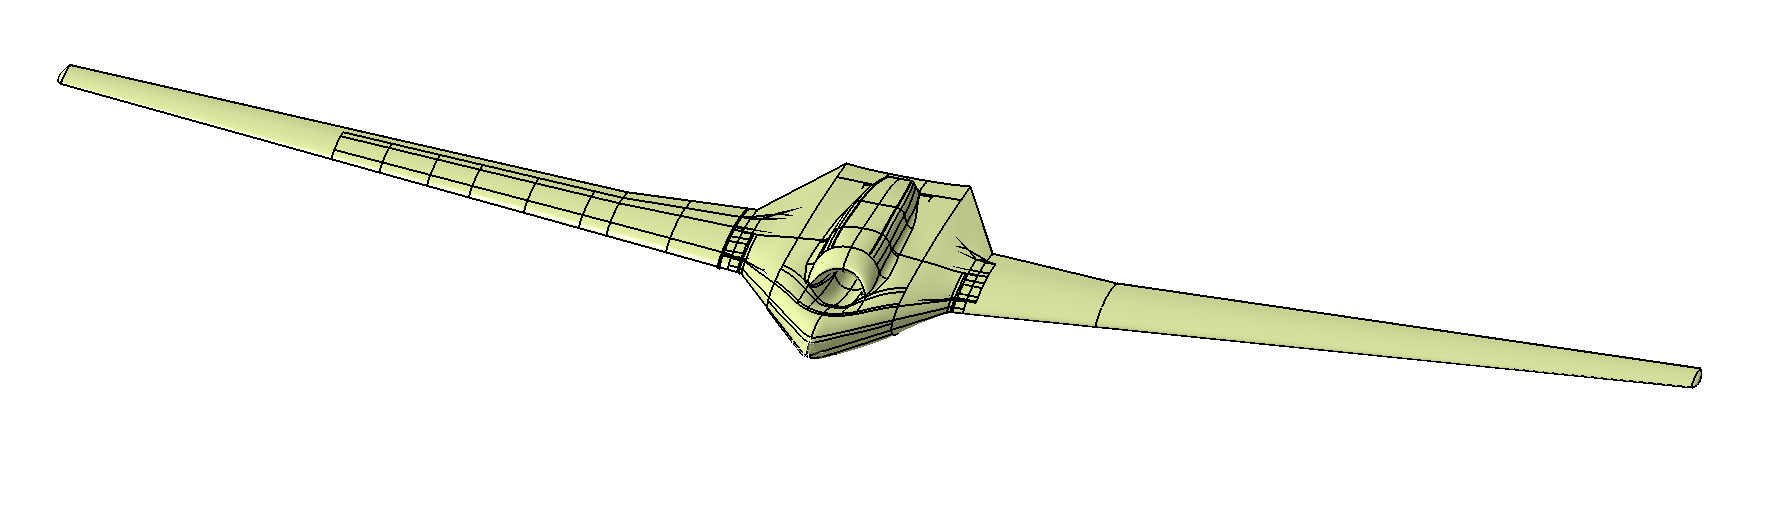
\includegraphics[width=1\textwidth]{BPS_Catia_Full}
\caption{Внешний вид гипотетической конструкции БПЛА}
\label{fig:BPLA_TSAGI}
\end{figure}

Конструкция выполнена по схеме ``бесхвостка'' с крылом большого удлинения и высокой степенью интегрированности крыла с фюзеляжем и двигателя с фюзеляжем. 

Для лучшей интеграции двигателя, включая воздухозаборник, в конструкцию БПЛА разработчикам пришлось использовать центроплан изогнутой формы (Рис.\ref{fig:OriginalSectionWithEngine}). Использование такой формы центроплана сопряжено с возможным возникновением новых проблем обеспечения прочности такого типа конструкции. Проблемы прочности в этом случае усугубляются из-за больших величин изгибающего момента, приходящего от крыла большого удлинения. 

Поскольку использование изогнутого центроплана может существенно ухудшить весовую эффективность БПЛА по сравнению с использованием прямого центроплана, для оценки величин этих весовых издержек необходимо проведение комплексных исследований по зависимости веса конструкции центроплана от геометрических параметров, характеризующих его кривизну. 
Необходимость таких исследований была связана с тем, что рассматриваемая в работе конструкция центроплана является нетрадиционной, и проведенный автором поиск конструкций прототипов не обнаружил наличия прямых прототипов данной конструкции центроплана для рассматриваемой размерности.

%Исследований центропланов такой формы ранее не проводилось.
 
%очевидно, что волнообразный центроплан может иметь напряжные вопросы с обеспечением прочности, т.к. такие центропланы в такой размерности не использовались, довольно нагружены. Сказать про компоновку, нарисовать её (общие вещи).

%с самого начала пишем, какие проблемы. Так сделали, такая компоновка, но у неё такие-то проблемы след волнообразный центроплан

%дальше: это может существенно ухудшить компоновку и весовую эффективность по сравнению с прямым центропланом. Цель работы - оценить возможные ухудшения. 

% и уже для того, чтобы оценить: следующий параграф 

Для оценки возможных ухудшений весовой эффективности конструкции центроплана необходимо построение расчетной прочностной модели гипотетической конструкции БПЛА, позволяющей проводить параметрический анализ зависимости прочности центроплана от геометрических параметров, определяющих его кривизну. Это необходимо и для последующего решения многодисциплинарной проектировочной задачи, в рамках которой будет возможность варьирования внешних аэродинамических обводов. 
Решение такой задачи предполагается осуществить в дальнейшем вне рамок данной работы. 

В настоящей (бакалаврской) работе не предполагается вариации внешних аэродинамических обводов и выхода этих параметров за пределы, определенные компоновкой "БПЛА-ЦАГИ", для которой они были выбраны из условия максимальной величины аэродинамического качества и минимума заметности, однако без учета требований прочности. 

%При построении модели необходимо было учесть ее дальнейшую модификацию, позволяющую варьировать форму внешних аэродинамических обводов. В бакалаврской работе форма внешних аэродинамических обводов постоянны. 


%Это скажем в разделе про нагрузки: Также постоянными считаются нагрузки на конструкцию (см.Раздел \ref{sec:externalLoads}). 

%В бакалаврской работе будем рассматривать только те обводы, которые есть в этой модели. И целью работы будет оценка потерь из-за такого центроплана (в прочности)

 
  
  

%Не забыть про то, что мы также хотим менять аэродинамику
%Требования: БПЛА, полет на таких-то высотах, столько-то. Весовая сводка такая-то, максимальные перегрузки, коэффициент запаса, аэродинамика. Ограничения - малозаметность, вес, пожаробезопасность отсека двигателя. 
%




\section{Компоновочная схема}
На рисунках 
\ref{fig:BPS_Catia_Top}--\ref{fig:BPS_Catia_Front} показана модель гипотетической конструкции БПЛА.


\begin{figure}[H]
\centering
\def\svgwidth{0.9\textwidth}
\input{figures/BPS_Catia_Top.pdf_tex}
\caption{Вид сверху}
\label{fig:BPS_Catia_Top}
\end{figure}

Как видно из рисунков для данной компоновочной схемы используется крыло большого удлинения. Из рисунка \ref{fig:BPS_Catia_WithoutSkin}, на котором представлена базовая конструктивно-силовая схема БПЛА, можно видеть, как происходит интеграция корпуса фюзеляжа, крыла и двигателя. 

\begin{figure}[H]
\centering
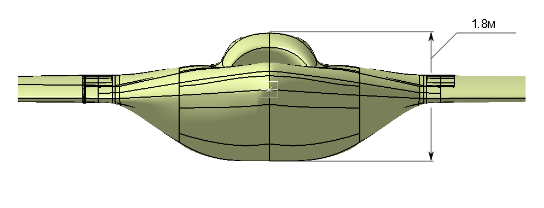
\includegraphics[width=0.8\textwidth]{BPS_Catia_Front}
\caption{Вид фюзеляжа спереди}
\label{fig:BPS_Catia_Front}
\end{figure}

\begin{figure}[H]
\centering
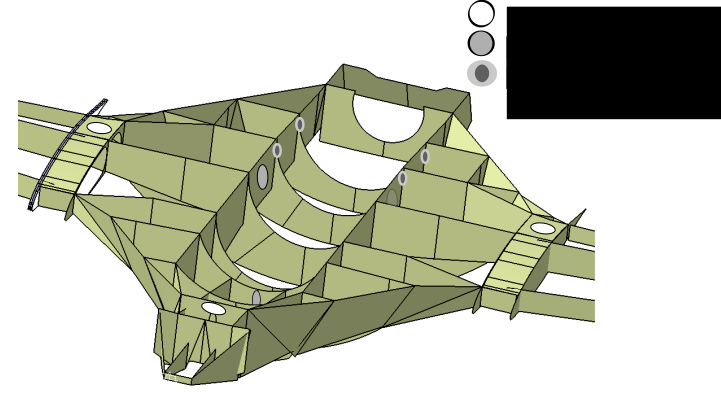
\includegraphics[width=0.8\textwidth]{BPS_Catia_WithoutSkin}
\caption{Вид фюзеляжа со снятой обшивкой}
\label{fig:BPS_Catia_WithoutSkin}
\end{figure}

%\begin{figure}[H]
%\centering
%\def\svgwidth{0.9\textwidth}
%\input{figures/BPS_Catia_WithoutSkin.pdf_tex}
%\caption{Вид фюзеляжа со снятой обшивкой с указанием узлов крепления шасси и двигателя}
%\label{fig:BPS_Catia_WithoutSkin}
%\end{figure}

Из рисунка видно, что двигатель с воздухозаборником значительно утоплены и находятся практически в середине фюзеляжа. Как уже отмечалось выше, эта особенность позволяет значительно улучшить малозаметность и аэродинамическое качество самолета (ссылка на отчет), но приводит к необходимости формировать искривленный центроплан. 

Формирование искривленного центроплана создает дополнительные проблемы из-за большой величины изгибающего момента в корне крыла. Еще одной проблемой обеспечения прочности корпуса БПЛА является высокая чувствительность параметров управляемости БПЛА от жесткостных характеристик корпуса и особенно зоны стыка крыла с центропланом, где расположены узлы крепления стоек основного шасси. Очевидно, что для решения проектировочной задачи необходимо проведение комплексных исследований прочности данной конструкции включая анализ прочности, устойчивости и управляемости. 

В данной схеме используется только горизонтальное оперение: руль высоты. Механизация крыла состоит из расщепляющихся элеронов на концах крыльев, элевонов и интерцепторов. В качестве тяги используется один реактивный двигатель, установленный в канале воздухозаборника. Места креплений стоек и замков шасси, расположение двигателя и узлов его крепления показаны на Рис. \ref{fig:BPS_Catia_Top_WithoutSkin}. 


\begin{figure}[H]
\centering
\def\svgwidth{0.9\textwidth}
\input{figures/BPS_Catia_Top_WithoutSkin.pdf_tex}
\caption{Вид сверху без обшивки с указанием узлов крепления шасси и двигателя}
\label{fig:BPS_Catia_Top_WithoutSkin}
\end{figure}

Отсеки фюзеляжа делятся на несколько групп по назначению. Распределение отсеков фюзеляжа по назначению представлено на Рис.\ref{fig:BPS_Catia_Top_PartRoles}. 

На рис.\ref{fig:BPS_Catia_Top_PartRoles} схематически показаны основные отсеки конструкции БПЛА. 

\begin{figure}[H]
\centering
\def\svgwidth{0.9\textwidth}
\input{figures/BPS_Catia_Top_PartRoles.pdf_tex}
\caption{Вид сверху с обозначением роли отсеков}
\label{fig:BPS_Catia_Top_PartRoles}
\end{figure}
	

\section{Внешние нагрузки}
\label{sec:externalLoads}
В работе исследуется прочность конструкции при случае нагружения A. Перегрузка $n_y = 2,97$, $M = 0,4$, скоростной напор $q = 503 \text{кгс}/\text{м}^2$, высота $H = 8\text{км}$. Нагрузки на конструкцию получены из работы \cite{BPS}, в которой были представлены расчетные нагрузки в диапазоне допускаемых режимов полета (см. Рис.\ref{fig:ModeOfFlight}). 
%описать режимы
Эпюры аэродинамических нагрузок представлены на Рис.\ref{fig:BendingMoments},\ref{fig:CuttingForces},\ref{fig:DistributedLoad}.



\begin{figure}[H]
\centering
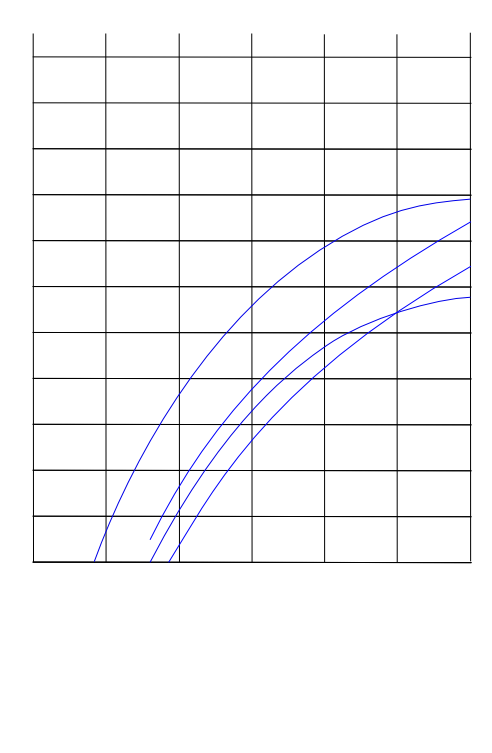
\includegraphics{HeightGraph}
\caption{Ограничения на режимы полета}
\label{fig:ModeOfFlight}
\end{figure}


\begin{figure}[H]
\centering
\def\svgwidth{0.7\textwidth}
\input{figures/BendingMoments.pdf_tex}
\caption{Эпюра изгибающих моментов}
\label{fig:BendingMoments}
\end{figure}

\begin{figure}[H]
\centering
\def\svgwidth{0.7\textwidth}
\input{figures/CuttingForces.pdf_tex}
\caption{Эпюра перерезывающих сил}
\label{fig:CuttingForces}
\end{figure}

\begin{figure}[H]
\centering
\def\svgwidth{0.7\textwidth}
\input{figures/DistributedLoad.pdf_tex}
\caption{Эпюра погонной нагрузки}
\label{fig:DistributedLoad}
\end{figure}

Как видно из имеющихся данных, влияние кручения на крыло невелико по сравнению с изгибом. В связи с этим в дальнейшем в работе будем пренебрегать кручением крыла, рассматривая только изгибные деформации. Где-то здесь будет график эпюры для кручения.




\section{Расчетные прочностные модели}
\section{Создание конечно-элементной модели проектируемого самолета}

В ходе работы были исследованы вопросы построения проектировочной модели БПЛА с крылом большого удлинения и несущим фюзеляжем. При помощи программного комплекса ``Conver'' (см. раздел \ref{sec:Conver}), исходя из концептуальной модели, предложенной конструкторами, была создана МКЭ-модель проектируемого БПЛА с исключенной верхней частью воздухозаборника, не несущей в себе силовых элементов. 

\begin{figure}[ht]
\centering
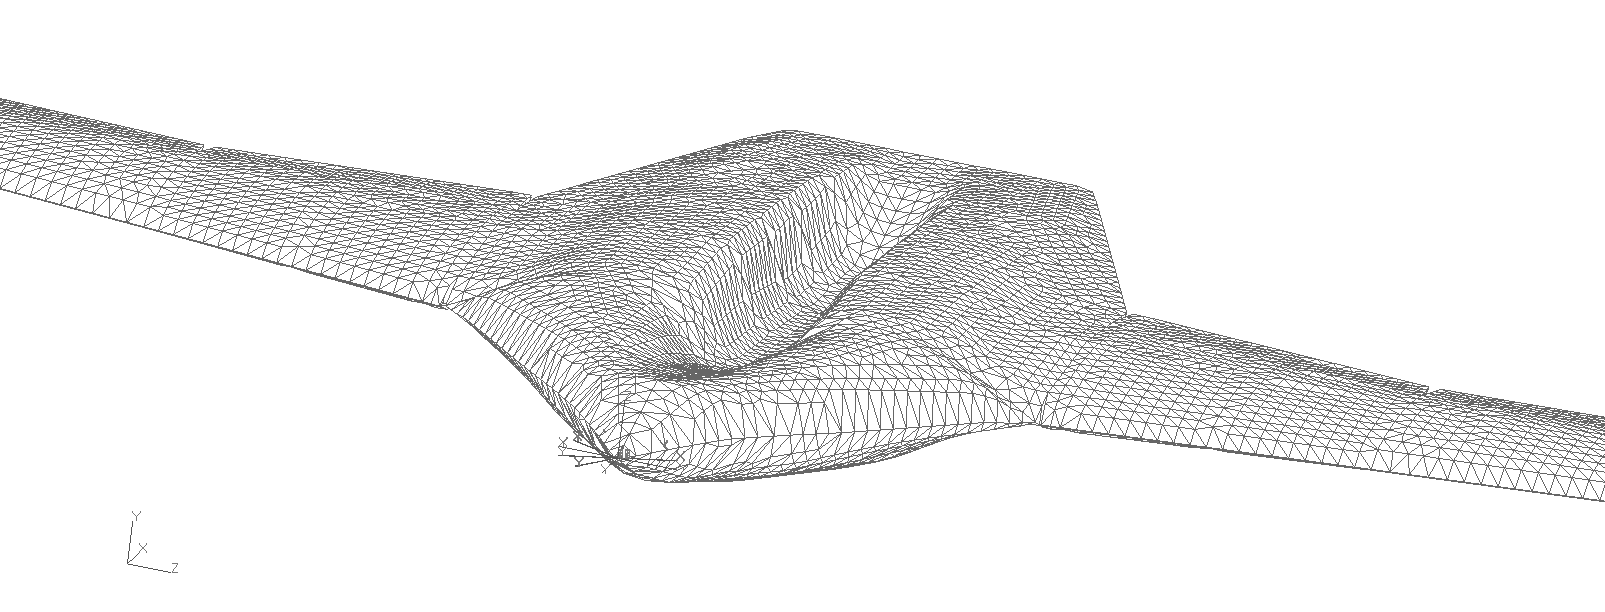
\includegraphics[width=0.8\textwidth]{BPLAfullModel}
\caption{МКЭ-модель проектируемого БПЛА без верхней части}
\label{fig:BPLAfullModel}
\end{figure}

\subsection{Подбор оптимальной дискретности модели}

В целях обеспечения точности расчета было проведено исследование зависимости напряженно-деформированного состояния самолета от максимального характерного размера конечных элементов, используемых в модели. 

С помощью программного комплекса ``Conver'' было построено 7 моделей самолета по одинаковой схеме с использованием различных размеров конечного элемента. Путем расчета моделей были определены средние величины напряжений для панелей и стенок в наиболее напряженных отсеках самолета (обозначены белым на  Рис.\ref{fig:WingRootPlain})

\begin{figure}[ht]
\centering
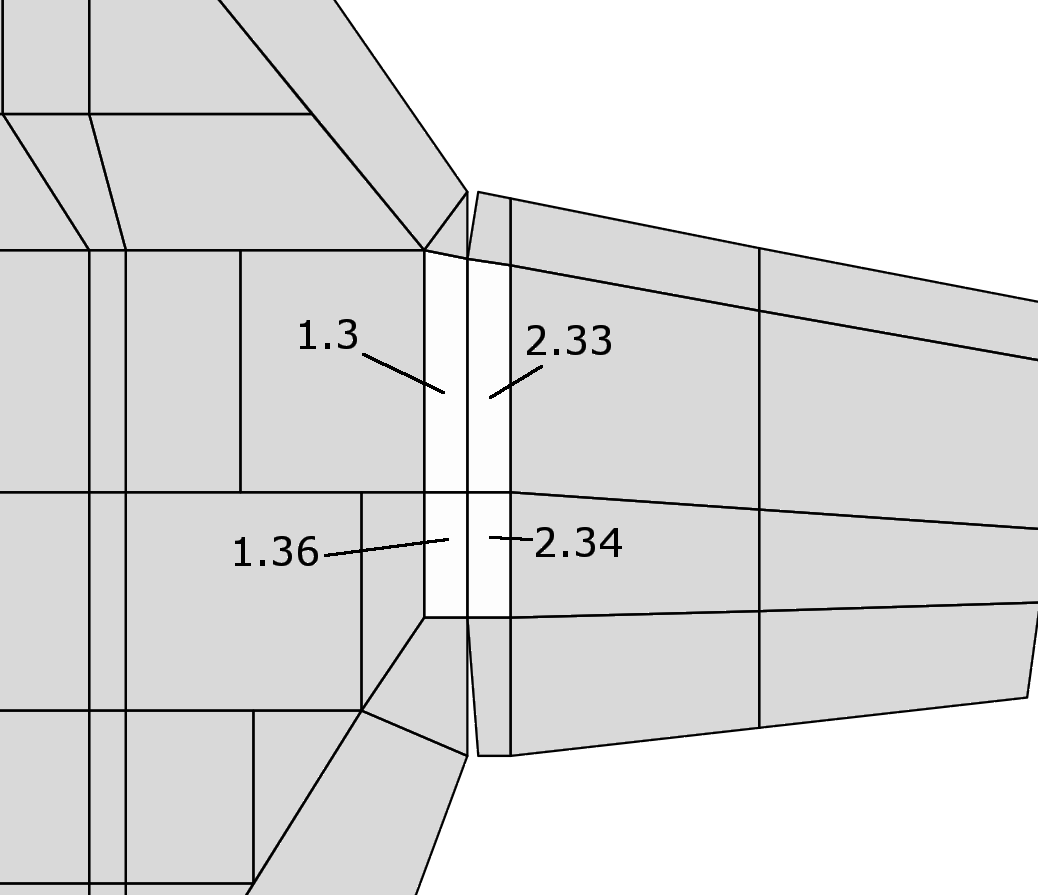
\includegraphics[width=0.5\textwidth]{RootOfWingWithSelectedPartsBW}
\caption{Схематичное изображение вида сверху в месте стыка правого крыла и фюзеляжа}
\label{fig:WingRootPlain}
\end{figure}




Исходя из полученных данных, была получена зависимость величины средних напряжений в панелях и стенках этих отсеков от выбора размера конечного элемента (Рис.\ref{fig:stressToDiscreteness})

\begin{figure}[ht]
\centering
%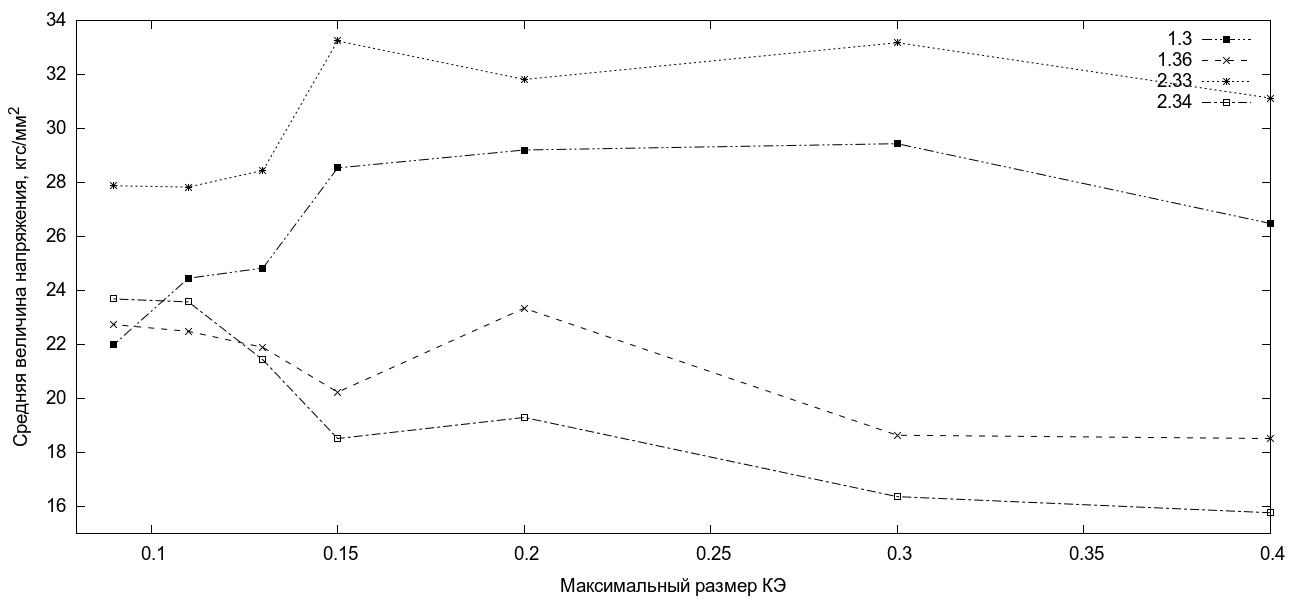
\includegraphics[width=0.8\textwidth]{StressToDiscretenessPlot}
% GNUPLOT: LaTeX picture with Postscript
\begingroup
  \makeatletter
  \providecommand\color[2][]{%
    \GenericError{(gnuplot) \space\space\space\@spaces}{%
      Package color not loaded in conjunction with
      terminal option `colourtext'%
    }{See the gnuplot documentation for explanation.%
    }{Either use 'blacktext' in gnuplot or load the package
      color.sty in LaTeX.}%
    \renewcommand\color[2][]{}%
  }%
  \providecommand\includegraphics[2][]{%
    \GenericError{(gnuplot) \space\space\space\@spaces}{%
      Package graphicx or graphics not loaded%
    }{See the gnuplot documentation for explanation.%
    }{The gnuplot epslatex terminal needs graphicx.sty or graphics.sty.}%
    \renewcommand\includegraphics[2][]{}%
  }%
  \providecommand\rotatebox[2]{#2}%
  \@ifundefined{ifGPcolor}{%
    \newif\ifGPcolor
    \GPcolorfalse
  }{}%
  \@ifundefined{ifGPblacktext}{%
    \newif\ifGPblacktext
    \GPblacktexttrue
  }{}%
  % define a \g@addto@macro without @ in the name:
  \let\gplgaddtomacro\g@addto@macro
  % define empty templates for all commands taking text:
  \gdef\gplbacktext{}%
  \gdef\gplfronttext{}%
  \makeatother
  \ifGPblacktext
    % no textcolor at all
    \def\colorrgb#1{}%
    \def\colorgray#1{}%
  \else
    % gray or color?
    \ifGPcolor
      \def\colorrgb#1{\color[rgb]{#1}}%
      \def\colorgray#1{\color[gray]{#1}}%
      \expandafter\def\csname LTw\endcsname{\color{white}}%
      \expandafter\def\csname LTb\endcsname{\color{black}}%
      \expandafter\def\csname LTa\endcsname{\color{black}}%
      \expandafter\def\csname LT0\endcsname{\color[rgb]{1,0,0}}%
      \expandafter\def\csname LT1\endcsname{\color[rgb]{0,1,0}}%
      \expandafter\def\csname LT2\endcsname{\color[rgb]{0,0,1}}%
      \expandafter\def\csname LT3\endcsname{\color[rgb]{1,0,1}}%
      \expandafter\def\csname LT4\endcsname{\color[rgb]{0,1,1}}%
      \expandafter\def\csname LT5\endcsname{\color[rgb]{1,1,0}}%
      \expandafter\def\csname LT6\endcsname{\color[rgb]{0,0,0}}%
      \expandafter\def\csname LT7\endcsname{\color[rgb]{1,0.3,0}}%
      \expandafter\def\csname LT8\endcsname{\color[rgb]{0.5,0.5,0.5}}%
    \else
      % gray
      \def\colorrgb#1{\color{black}}%
      \def\colorgray#1{\color[gray]{#1}}%
      \expandafter\def\csname LTw\endcsname{\color{white}}%
      \expandafter\def\csname LTb\endcsname{\color{black}}%
      \expandafter\def\csname LTa\endcsname{\color{black}}%
      \expandafter\def\csname LT0\endcsname{\color{black}}%
      \expandafter\def\csname LT1\endcsname{\color{black}}%
      \expandafter\def\csname LT2\endcsname{\color{black}}%
      \expandafter\def\csname LT3\endcsname{\color{black}}%
      \expandafter\def\csname LT4\endcsname{\color{black}}%
      \expandafter\def\csname LT5\endcsname{\color{black}}%
      \expandafter\def\csname LT6\endcsname{\color{black}}%
      \expandafter\def\csname LT7\endcsname{\color{black}}%
      \expandafter\def\csname LT8\endcsname{\color{black}}%
    \fi
  \fi
  \setlength{\unitlength}{0.0500bp}%
  \begin{picture}(8502.00,4534.00)%
    \gplgaddtomacro\gplbacktext{%
      \csname LTb\endcsname%
      \put(814,892){\makebox(0,0)[r]{\strut{} 16}}%
      \put(814,1267){\makebox(0,0)[r]{\strut{} 18}}%
      \put(814,1642){\makebox(0,0)[r]{\strut{} 20}}%
      \put(814,2017){\makebox(0,0)[r]{\strut{} 22}}%
      \put(814,2393){\makebox(0,0)[r]{\strut{} 24}}%
      \put(814,2768){\makebox(0,0)[r]{\strut{} 26}}%
      \put(814,3143){\makebox(0,0)[r]{\strut{} 28}}%
      \put(814,3518){\makebox(0,0)[r]{\strut{} 30}}%
      \put(814,3894){\makebox(0,0)[r]{\strut{} 32}}%
      \put(814,4269){\makebox(0,0)[r]{\strut{} 34}}%
      \put(1393,484){\makebox(0,0){\strut{} 0.1}}%
      \put(2512,484){\makebox(0,0){\strut{} 0.15}}%
      \put(3631,484){\makebox(0,0){\strut{} 0.2}}%
      \put(4749,484){\makebox(0,0){\strut{} 0.25}}%
      \put(5868,484){\makebox(0,0){\strut{} 0.3}}%
      \put(6986,484){\makebox(0,0){\strut{} 0.35}}%
      \put(8105,484){\makebox(0,0){\strut{} 0.4}}%
      \put(176,2486){\rotatebox{-270}{\makebox(0,0){\strut{}Средняя величина напряжения, $\text{кгс}/\text{мм}^2$}}}%
      \put(4525,154){\makebox(0,0){\strut{}Максимальный размер КЭ}}%
    }%
    \gplgaddtomacro\gplfronttext{%
      \csname LTb\endcsname%
      \put(7118,4096){\makebox(0,0)[r]{\strut{}$1.3$}}%
      \csname LTb\endcsname%
      \put(7118,3876){\makebox(0,0)[r]{\strut{}$1.36$}}%
      \csname LTb\endcsname%
      \put(7118,3656){\makebox(0,0)[r]{\strut{}$2.33$}}%
      \csname LTb\endcsname%
      \put(7118,3436){\makebox(0,0)[r]{\strut{}$2.34$}}%
    }%
    \gplbacktext
    \put(0,0){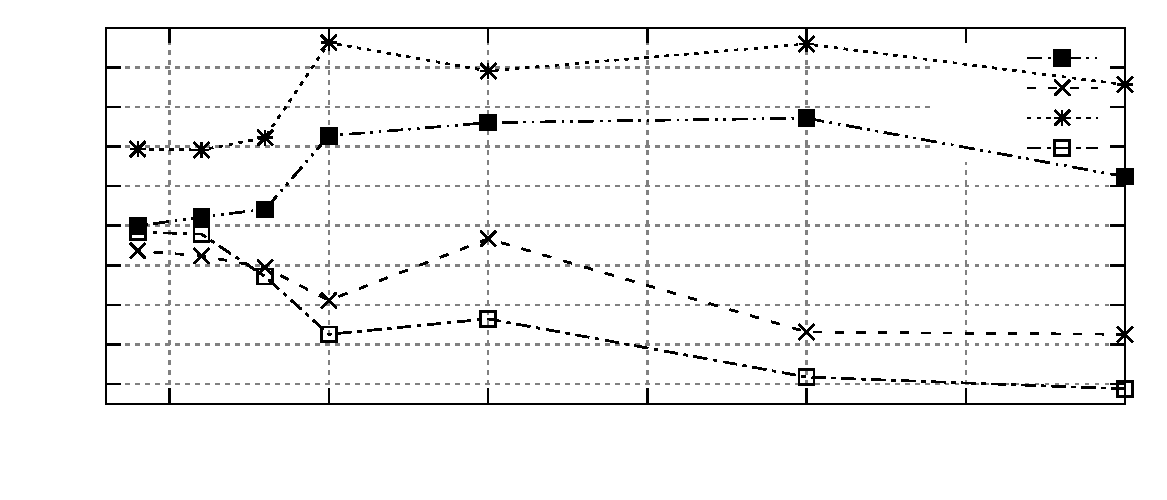
\includegraphics{StressToDiscreteness}}%
    \gplfronttext
  \end{picture}%
\endgroup

\caption{Зависимость средних напряжений в отсеках от величины КЭ}
\label{fig:stressToDiscreteness}
\end{figure}

На основании полученных данных и исходя из трудоемкости процесса расчета модели была определена оптимальная величина конечного элемента для дальнейшей работы над моделью, принятая равной $0,11\text{м}$. 
%Ниже приведены картины НДС в месте стыка крыла с фюзеляжем при различных размерах конечного элемента. 



\section{Результаты расчетов НДС конструкции БПЛА} 
\label{sec:ndsResults}
%\subsection{Проблемы проектирования}

С помощью сформированной расчетной МКЭ-модели были проведены прочностные исследования напряженно-деформированного состояния(НДС) модели гипотетического БПЛА в рамках проектировочного исследования по определению рациональных параметров конструкции центроплана. 
Из-за существенного влияния жесткостных параметров конструкции планера БПЛА на прочностные параметры конструкции центроплана это проектировочное исследование включало всю первичную конструкцию БПЛА. На основе начальных данных, полученных аналитическим способом, была проведена оптимизация толщин панелей и стенок отсеков для нахождения минимальной по весу конструкции, удовлетворяющей требованиям прочности. Условия по устойчивости анализировались в автоматическом режиме лишь для подкрепленных панелей центроплана и кессона крыла.

Для модели, полученной в результате определения рациональных параметров, можно выделить следующие особенности НДС:

\begin{enumerate}
\item Усилия в обшивке фюзеляжа оказались относительно малы за исключением обшивки центроплана. Поэтому большая часть обшивки имела минимальную толщину, определяемую геометрическими и технологическими ограничениями.
\item Наибольшие усилия наблюдались в центроплане и в корне крыла. Так, в корне крыла наблюдались следующие величины усилий: $Q = 13,7~\text{тс}$, $M_\text{изг} = 80~\text{тс}\cdot\m$. 
\item Значительные усилия наблюдались в стенках отсека двигателя в местах крепления двигателя (дополнительный анализ этой особенности произведен далее в данном разделе). 
\item Влияние кручения крыла мало относительно изгиба крыла. На Рис.\ref{fig:WingDeformation3},\ref{fig:WingRotating} показаны эпюры прогибов лонжеронов при изгибе и кручении крыла.
\end{enumerate}  

Общая картина НДС расчетной модели БПЛА представлена на Рис.\ref{fig:patranRearDeformed}--\ref{fig:patranTopIsoWithoutSk}


\begin{figure}[H]
\centering

\captionsetup{justification=centering}
\def\svgwidth{0.9\textwidth}
\input{figures/WingDeformation3.pdf_tex}
\caption{Эпюра прогиба кессона крыла}
\label{fig:WingDeformation3}
\end{figure}

\begin{figure}[H]
\centering
\def\svgwidth{0.9\textwidth}
\input{figures/WingRotating.pdf_tex}
\caption{Кручение крыла. Разность прогибов лонжеронов}
\label{fig:WingRotating}
\end{figure}


\begin{figure}[H]
\centering
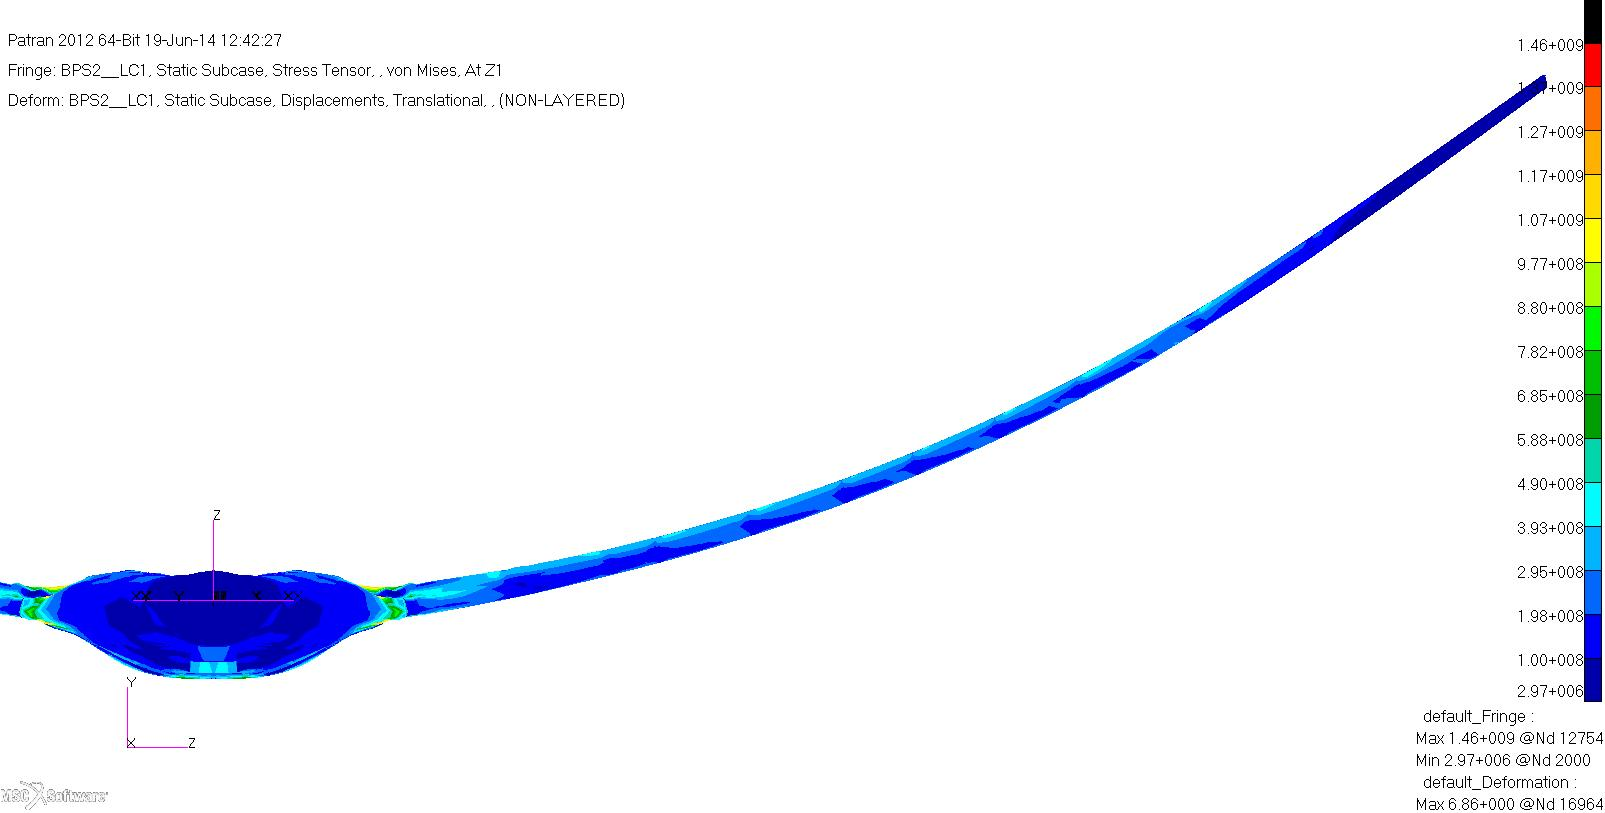
\includegraphics[width=0.8\textwidth]{patran/rear_deformed}
\caption{НДС конструкции гипотетического БПЛА. Вид сзади}
\label{fig:patranRearDeformed}
\end{figure}


%\begin{figure}[H]
%\centering
%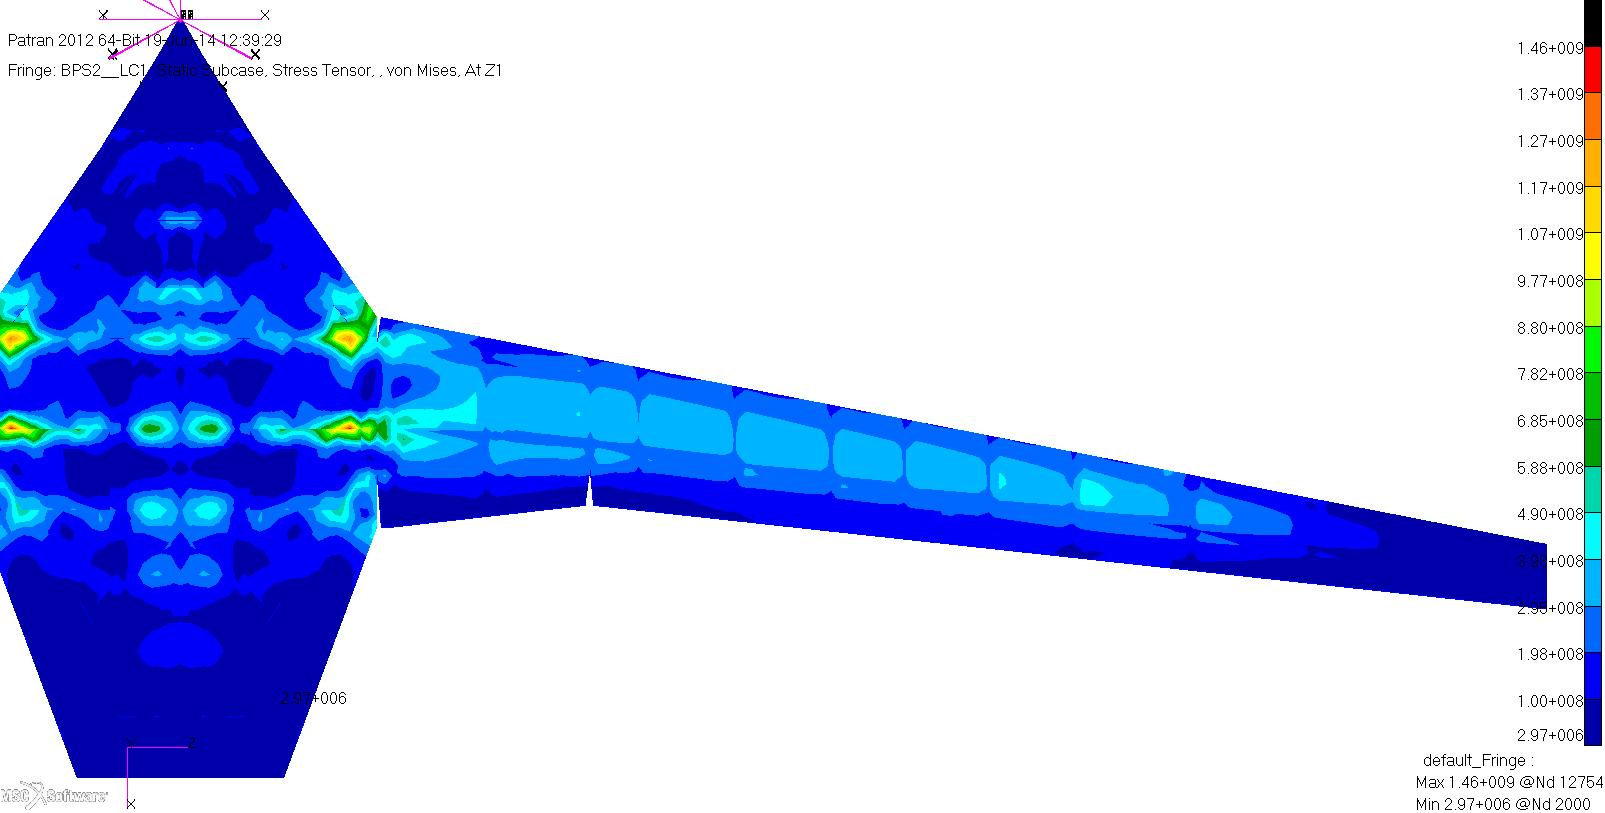
\includegraphics[width=0.7\textwidth]{patran/bottom}
%\caption{НДС конструкции гипотетического БПЛА. Вид снизу}
%\label{fig:patranBottom}
%\end{figure}
%
%
%\begin{figure}[H]
%\centering
%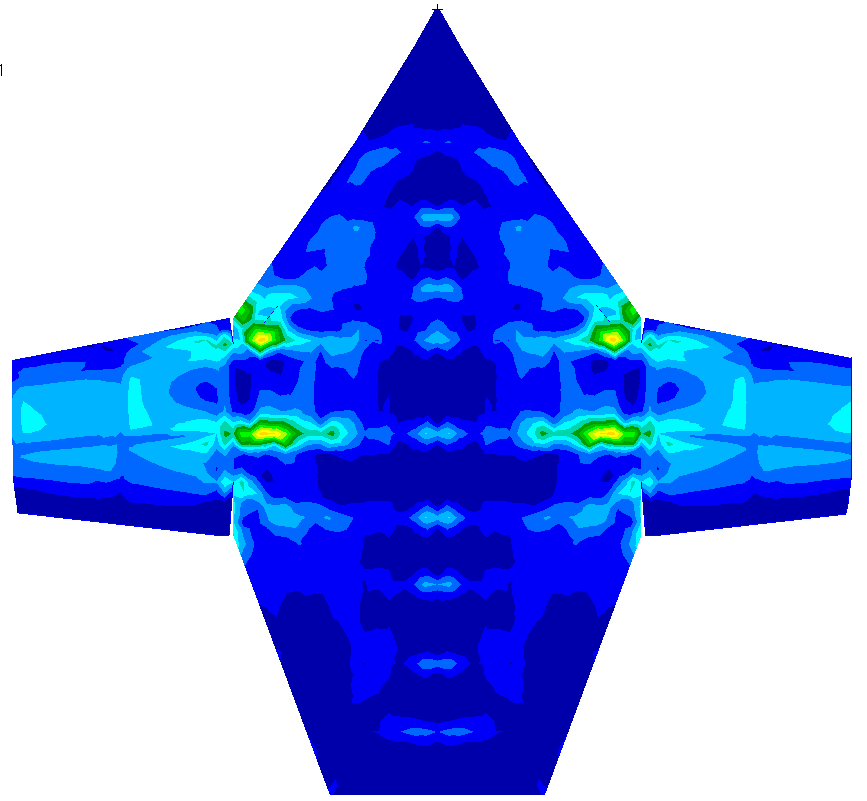
\includegraphics[width=0.7\textwidth]{patran/top}
%\caption{НДС конструкции гипотетического БПЛА. Вид сверху}
%\label{fig:patranTop}
%\end{figure}


\begin{figure}[H]
\centering
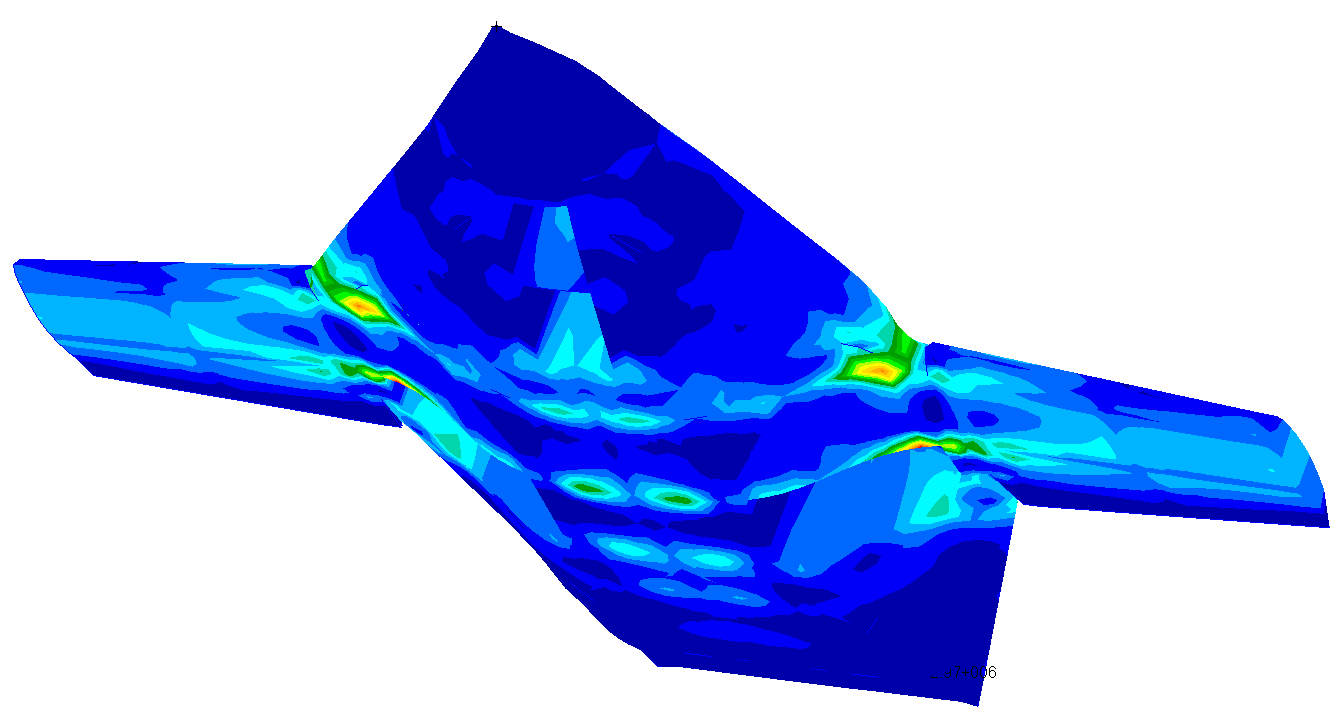
\includegraphics[width=0.8\textwidth]{patran/bottom_iso}
\caption{НДС конструкции гипотетического БПЛА. Вид в изометрии снизу}
\label{fig:patranBottomIso}
\end{figure}

\begin{figure}[H]
\centering
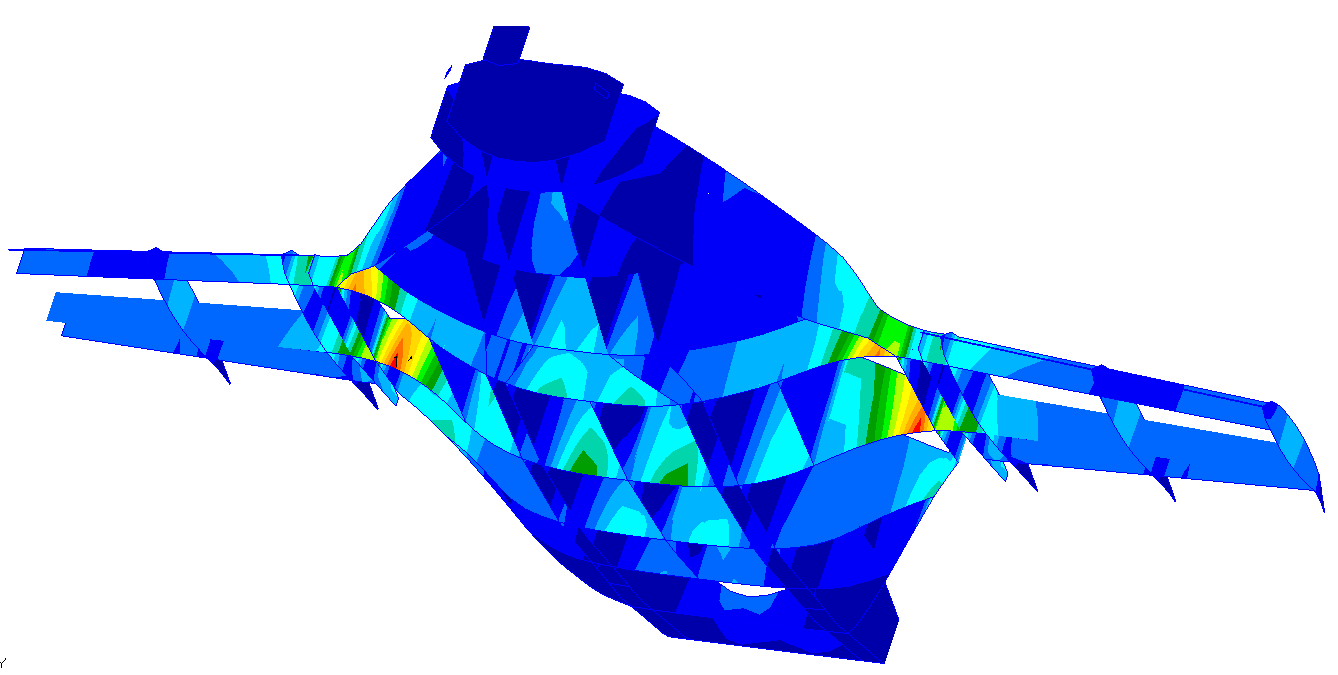
\includegraphics[width=0.8\textwidth]{patran/bottom_iso_noskin}
\caption{НДС конструкции гипотетического БПЛА. Вид снизу в изометрии без обшивки}
\label{fig:patranBottomIsoWithoutSkin}
\end{figure}

\begin{figure}[H]
\captionsetup{justification=centering}
\centering
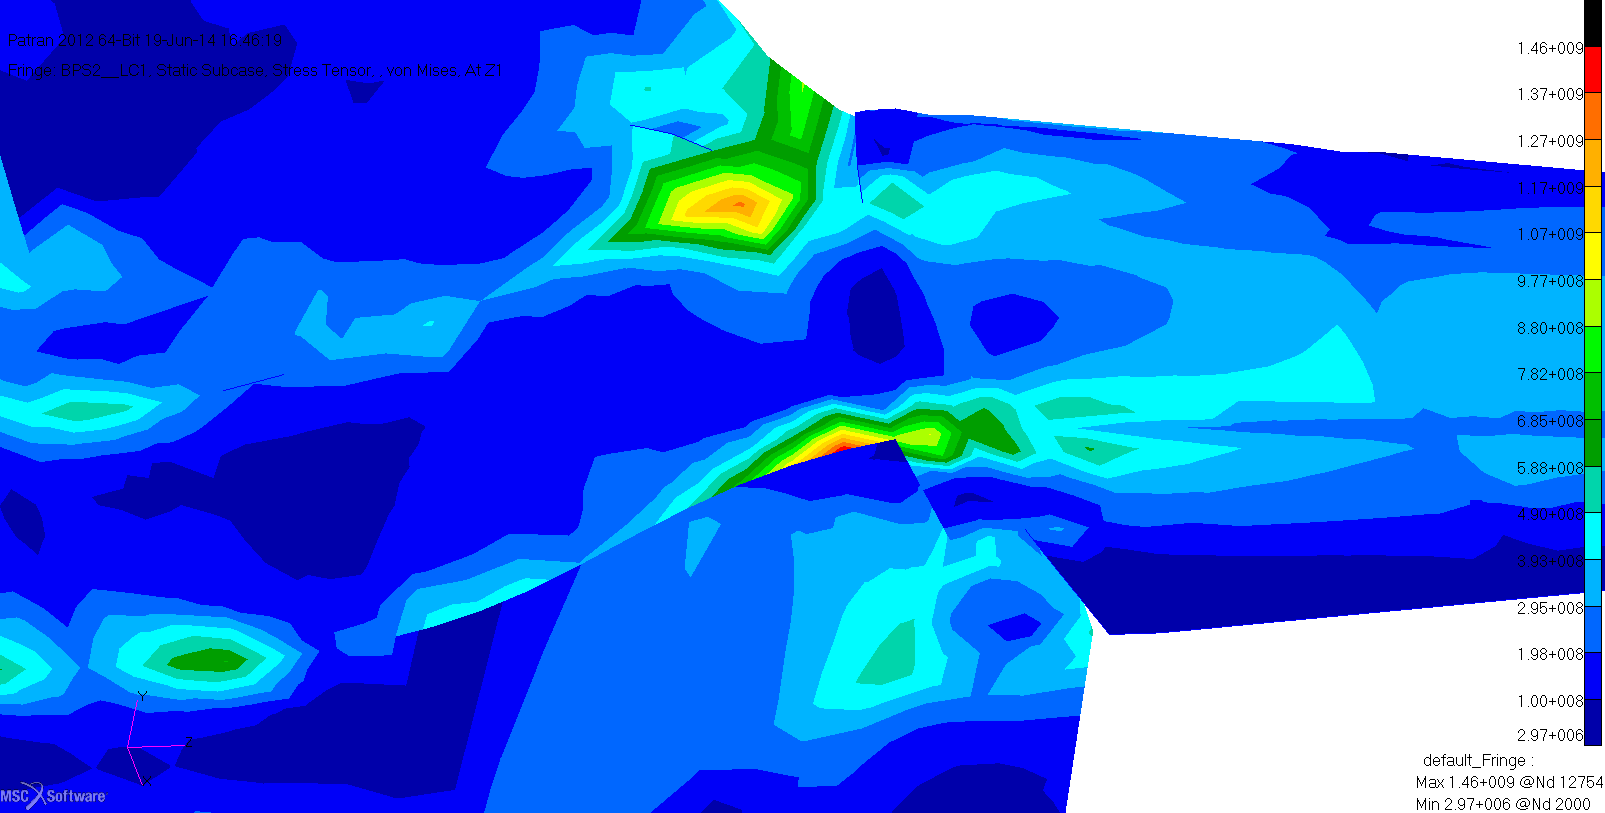
\includegraphics[width=0.8\textwidth]{patran/bottom_zoom}
\caption{НДС конструкции гипотетического БПЛА. Вид на стык крыла с фюзеляжем снизу в изометрии}
\label{fig:patranBottomIsoZoom}
\end{figure}


\begin{figure}[H]
\centering
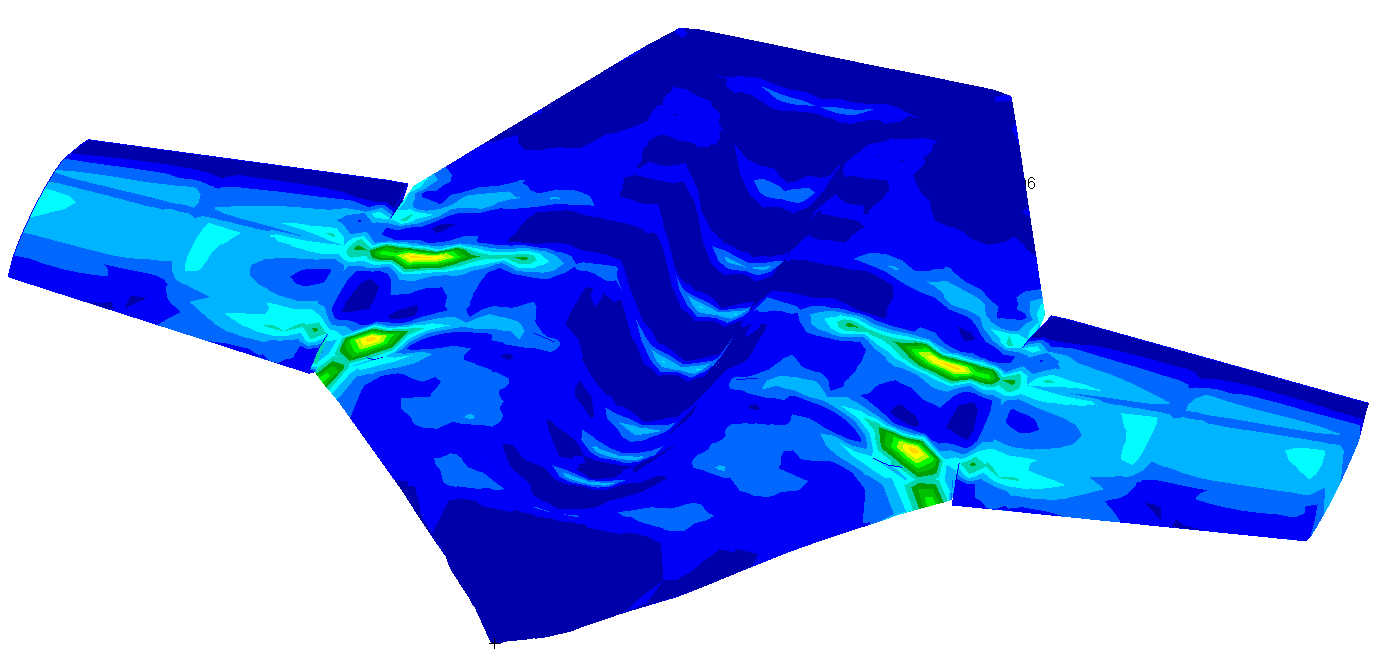
\includegraphics[width=0.8\textwidth]{patran/top_iso}
\caption{НДС конструкции гипотетического БПЛА. Вид сверху в изометрии}
\label{fig:patranTopIso}
\end{figure}

\begin{figure}[H]
\centering
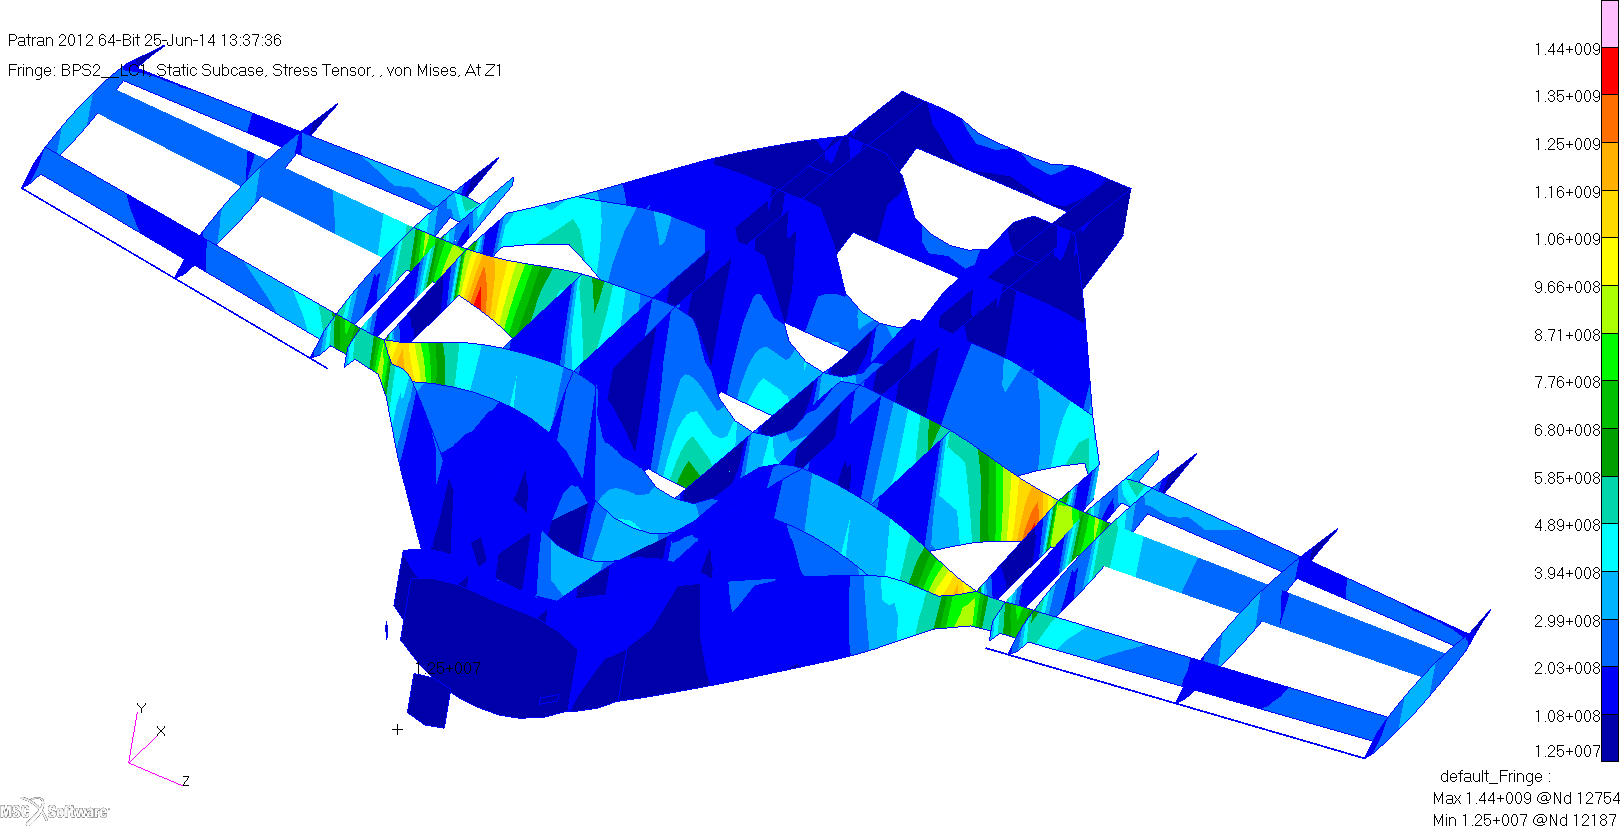
\includegraphics[width=0.8\textwidth]{patran/top_iso_noskin}
\caption{НДС конструкции гипотетического БПЛА. Вид сверху в изометрии без обшивки}
\label{fig:patranTopIsoWithoutSk}
\end{figure}
 \paragraph{Крепление хвостовой части к кессону центроплана} 
\label{sec:pants}
\begin{figure}[H]
\centering
\def\svgwidth{\textwidth}
\input{figures/IsoviewOfPants.pdf_tex}
%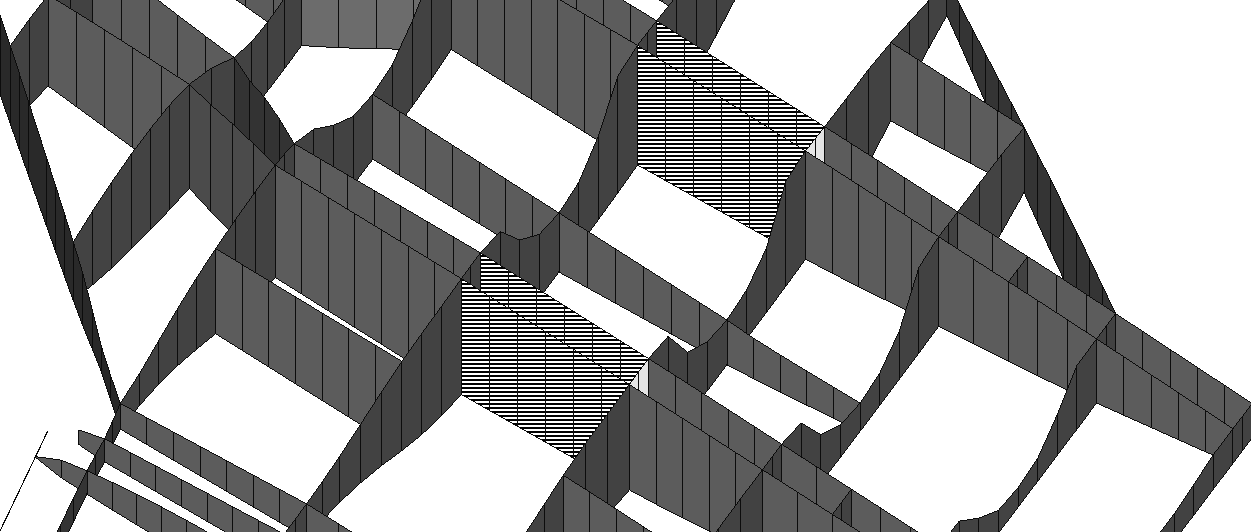
\includegraphics[width=0.6\textwidth]{IsoviewOfPantsBW}
\caption{Вид каркаса фюзеляжа}
\label{fig:IsoviewOfPants}
\end{figure}


Для частичной валидации решения, полученного в результате определния рациональных параметров (см. предыдущий раздел), была решена модельная задача по оценке устойчивости центральных стенок, обеспечивающих крепление хвостовой части гипотетического БПЛА к его центроплану (данные стенки обозначены на Рис.~\ref{fig:IsoviewOfPants} серой заливкой, светло-серой заливкой обозначены зоны основных узлов крепления двигателя). Эти стенки были нагружены перерезывающими усилиями, и необходима была проверка их по условиям устойчивости, которая не проводилась для этих элементов конструкции в процессе определения рациональных параметров. НДС стенок был оценен на основе аналитических формул. Схема нагружения модельных стенок показана на Рис.\ref{fig:IsoviewOfPantsModel}.

\begin{figure}[H]
\centering
%\def\svgwidth{0.9\textwidth}
\input{figures/IsoviewOfPantsModel.pdf_tex}
\caption{Схема нагружения модельных стенок}
\label{fig:IsoviewOfPantsModel}
\end{figure}

%
%\begin{figure}[H]
%\centering
%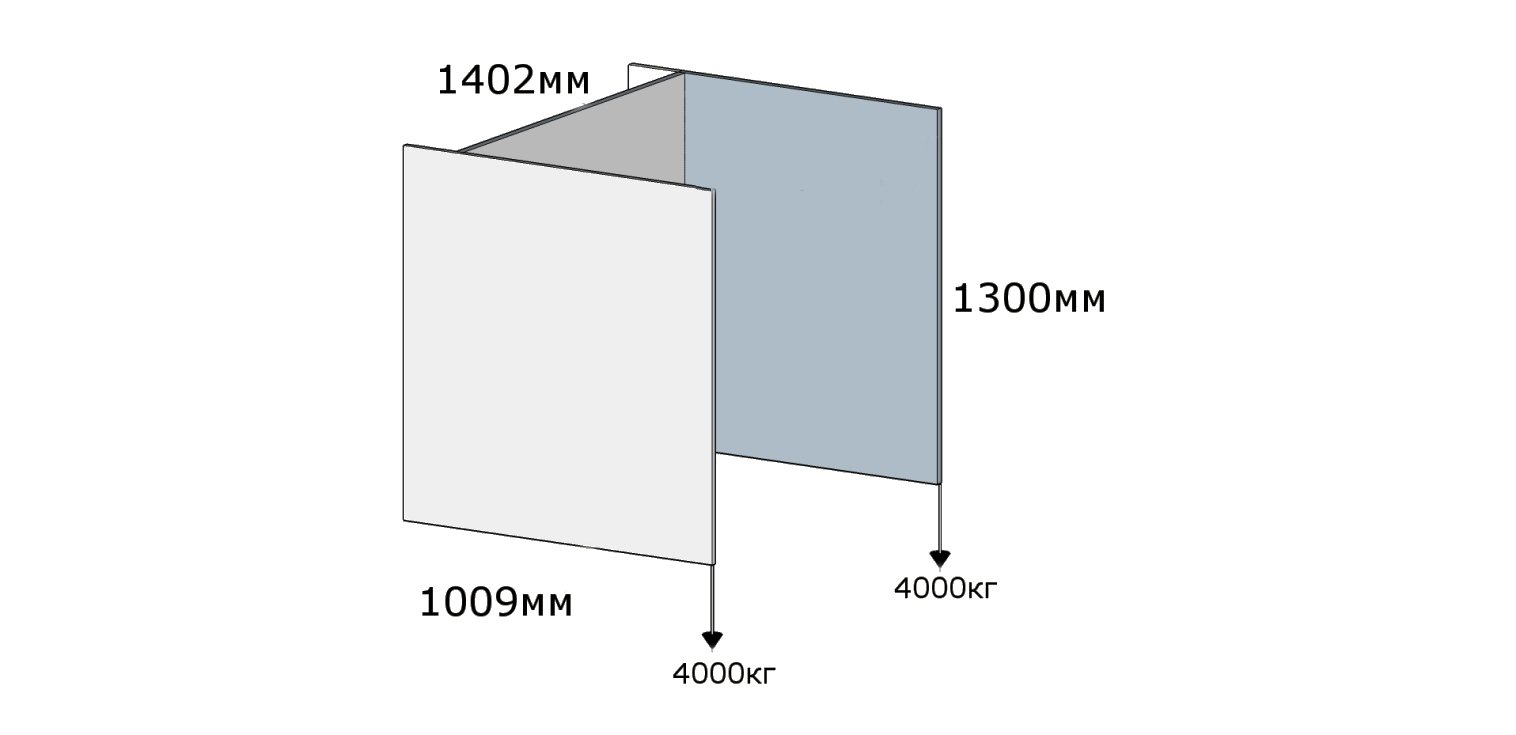
\includegraphics[width=0.8\textwidth]{IsoviewOfPantsModel}
%\caption{Схема нагружения модельных стенок}
%\label{IsoviewOfPantsModel}
%\end{figure}


Уровень нагружения был оценен по величинам касательных напряжений. Касательные напряжения в пластине при чистом сдвиге равны

\begin{equation}
\tau=\frac{3}{2}\cdot\frac{Q}{bh}
\end{equation}
Критические по устойчивости касательные напряжения в пластине при чистом сдвиге равны \cite{Volmir}:

\begin{equation}
\tau_\text{кр}=\frac{K}{12}\frac{\pi^2D}{b^2h} = \frac{K}{12}\frac{\pi^2E}{(1-\mu^2)}\left(\frac{h}{b}\right)^2,\, K=5.34 + 4\frac{a}{b},
\end{equation}
где $a$ - размер пластины вдоль направления действия силы, $b$ - размер пластины поперек направления действия силы, $h$ - толщина пластины, $D$ - изгибная жесткость пластины, $E$ - модуль Юнга, $\mu$ - модуль Пуассона материала пластины, $Q$ - приложенная сила.
Допускаемые толщины найдем из условия:

\begin{equation}
\tau_\text{кр} \geq \tau  
\end{equation}

\begin{equation}
h \geq \sqrt[3]{\frac{3\cdot12}{2}\frac{Qb\cdot(1-\mu^2)}{k\pi^2E}}
\end{equation}

Подставляя значения, получим:

\begin{equation}
Q=\frac{8000}{n}\text{кгс},\,a=1300\text{мм},\,b=1009\text{мм},\,\mu=0.3,\,E=7000\frac{\text{кгс}}{\text{мм}^2}
\end{equation}

\begin{equation}
h \geq \sqrt[3]{\frac{18\cdot8000\cdot1000\cdot(1-\mu^2)}{k\pi^2En}} = \frac{5.67}{\sqrt[3]{n}} 
\end{equation}

Таким образом, для случаев $n = 2$ и $n = 4$  были получены минимальные допустимые толщины, 
равные:

\begin{equation}
h\geq4.50\text{мм},\,n=2
\end{equation}
\begin{equation}
h\geq2.83\text{мм},\,n=4
\label{eq:pants_n4}
\end{equation}

Рациональные значения толщин исследуемых обшивок, полученные в данном проектировочном исследовании, оказались меньше ($h = 1\text{мм}$), чем приведенные в \ref{eq:pants_n4}. Таким образом, выполнение условий по устойчивости этих стенок привело к увеличению их толщин. Более рациональным способом увеличения сдвиговой жесткости этих стенок является использование ферменных подкрепляющих элементов.
%\subsubsection{Фюзеляжная часть центроплана}

Другим проблемным местом была фюзеляжная часть центроплана. Из-за требований компоновки, а именно интеграции двигателя, центроплан необходимо делать изогнутым (Рис.\ref{fig:centroplan}). Это вносит дополнительные трудности в виде увеличения веса по сравнению с прямым центропланом. Исследованию фюзеляжной части центроплана (выделена серым на Рис.\ref{fig:centroplan}) посвящена глава \ref{chap:SolvingModel}.

\begin{figure}[ht]
\centering
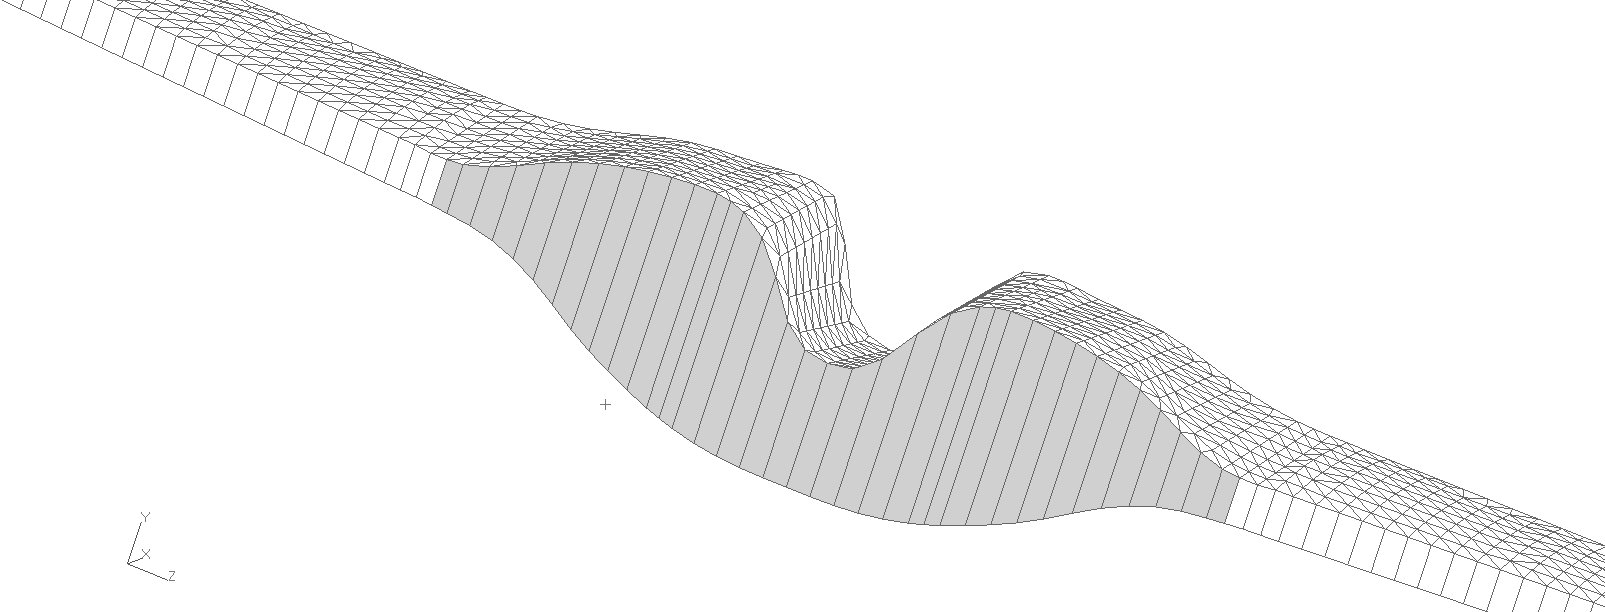
\includegraphics[width=0.6\textwidth]{centroplan}
\caption{Изогнутый центроплан с выделением исследуемой части}
\label{fig:centroplan}
\end{figure}


\section{Рациональные параметры КСС фюзеляжа}
На основе полученных в разделе \ref{sec:creationOfOneModel} данных была проведена оптимизация толщин стенок отсеков и панелей для выполнения требований прочности конструкции. Эпюры толщин верхних и нижних панелей центроплана, а также эпюры погонных усилий $N_1$ в верхних и нижних панелях центроплана представлены на Рис. \ref{fig:epures}

\begin{figure}[H]
\centering
\captionsetup{justification=centering}
\begin{subfigure}[b]{0.49\textwidth}
	\centering
	\def\svgwidth{\textwidth}
	\footnotesize
	\input{figures/EpureDistributedLoadN1Top.pdf_tex}	
	\normalsize
	%\label{fig:epureloadn1top}
	\caption{Эпюра погонных усилий $N_1$ в верхних панелях центроплана}
\end{subfigure}
\begin{subfigure}[b]{0.49\textwidth}
	\centering
	\def\svgwidth{\textwidth}
	\input{figures/EpureDistributedLoadN1Bottom.pdf_tex}
	%\label{fig:epureloadn1bottom}
	\caption{Эпюра погонных усилий $N_1$ в нижних панелях центроплана}
\end{subfigure}
\begin{subfigure}[b]{0.49\textwidth}
	\centering
	\def\svgwidth{\textwidth}
	\input{figures/EpureDistributedWeightTop.pdf_tex}
	%\label{fig:epureweighttop}
	\caption{Эпюра погонного веса верхних панелей центроплана}
\end{subfigure}
\begin{subfigure}[b]{0.49\textwidth}
	\centering
	\def\svgwidth{\textwidth}		\input{figures/EpureDistributedWeightBottom.pdf_tex}
	%\label{fig:epureweightbottom}
	\caption{Эпюра погонного веса нижних панелей центроплана}
\end{subfigure}
	\caption{Эпюры погонных усилий $N_1$ и погонного веса для верхних и нижних панелей центроплана}
	\label{fig:epures}
\end{figure}
%
%
%\begin{figure}[H]
%\centering
%\begin{subfigure}[b]{0.7\textwidth}
%	\centering
%	\def\svgwidth{\textwidth}
%	\input{figures/EpureDistributedLoadN2Top.pdf_tex}
%	\label{fig:epure:loadn2top}
%	\caption{Верхние панели}
%\end{subfigure}
%\begin{subfigure}[b]{0.7\textwidth}
%	\centering
%	\def\svgwidth{\textwidth}	\input{figures/EpureDistributedLoadN2Bottom.pdf_tex}
%	\label{fig:epure:loadn2bottom}
%	\caption{Нижние панели}
%\end{subfigure}
%\label{fig:epure:loadn2}
%\caption{Эпюра $N_y$}
%\end{figure}
%
%\begin{figure}
%	\centering
%	\def\svgwidth{\textwidth}
%	\input{figures/EpureDistributedLoadN12Bottom.pdf_tex}
%	\label{fig:epure:loadn12bottom}
%	\caption{Эпюра $N_\text{xy}$. Нижние панели}
%\end{figure}
%
%\begin{figure}
%	\centering
%	\def\svgwidth{\textwidth}
%	\input{figures/EpureDistributedLoadN12Top.pdf_tex}
%	\label{fig:epure:loadn12top}
%	\caption{Эпюра $N_\text{xy}$. Верхние панели}
%\end{figure}



%Параметры оптимизированной модели представлены в таблице \ref{tab:paramsOfOptimizedScheme}

%Остальные две главы будут как приложение к этой мощной главе: исследование влияния искривления кессона центроплана на его вес, выбор рациональной КСС.


\chapter{Исследование центроплана}
\label{chap:Kesson}

\section{Создание параметрической модели центроплана}
\label{sec:creationOfModel}

В рамках решения данной модельной задачи на базе общей МКЭ-модели гипотетической конструкции БПЛА (Рис.\ref{fig:fullMKE}) была создана упрощенная параметрическая модель центроплана, представляющая из себя подробную МКЭ-модель центроплана. В упрощенной модели кессон фюзеляжной части центроплана (Рис.\ref{fig:centroplanMKE}) заменен коробом переменного прямоугольного сечения с поперечными стенками. На короб передаются усилия аналогичные усилиям, приходящим с крыла для конструкции гипотетического БПЛА, путем приложения аэродинамических нагрузок на упрощенную модель крыла -- короб постоянного прямоугольного сечения (Рис.\ref{fig:simplifiedCentroplanMKE}). Материал - дюраль, панели и стенки центропланов имеют постоянную по площади толщину, без вырезов. Носовая и хвостовая части самолета опущены для простоты расчета.  


\begin{figure}[ht]
\centering 
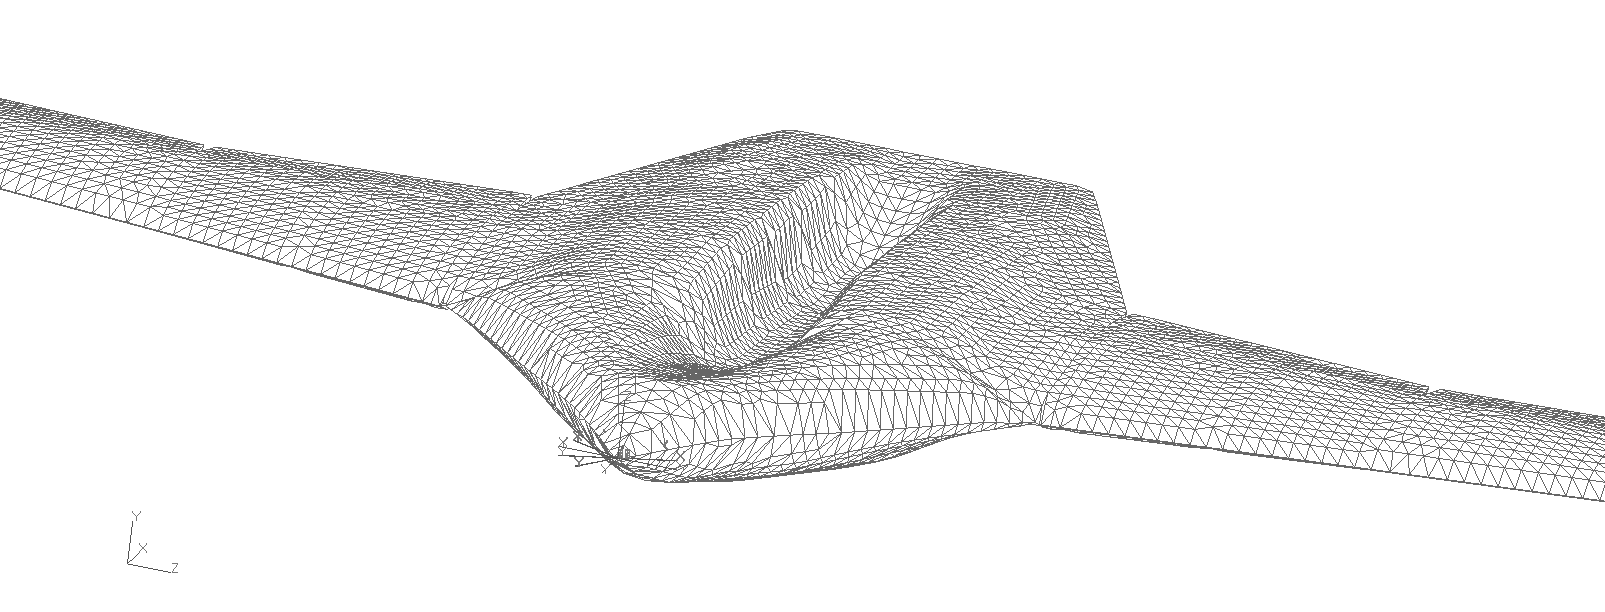
\includegraphics[width=0.9\textwidth]{BPLAfullModel}
\caption{МКЭ-модель гипотетической конструкции БПЛА}
\label{fig:fullMKE}
\end{figure}

\begin{figure}[ht]
\centering 
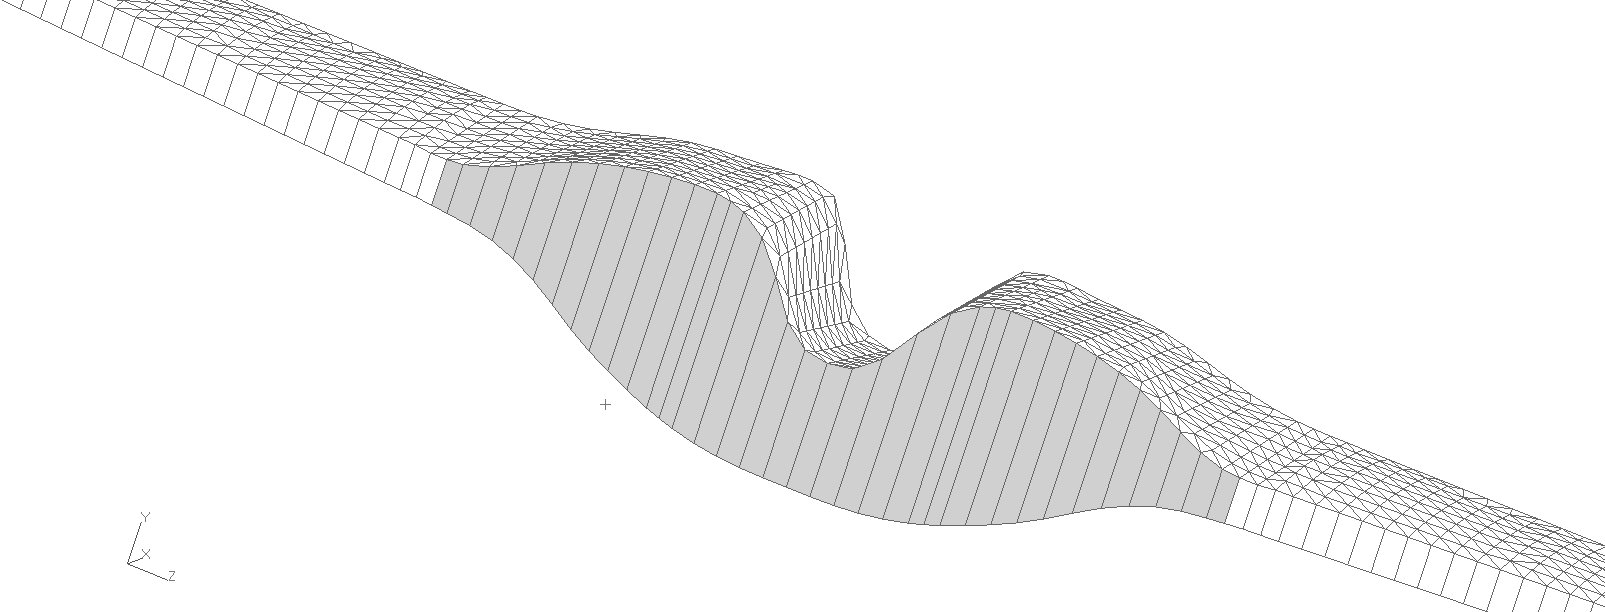
\includegraphics[width=0.9\textwidth]{centroplan}
\caption{МКЭ-модель центроплана гипотетической конструкции БПЛА}
\label{fig:centroplanMKE}
\end{figure}

\begin{figure}[ht]
\centering
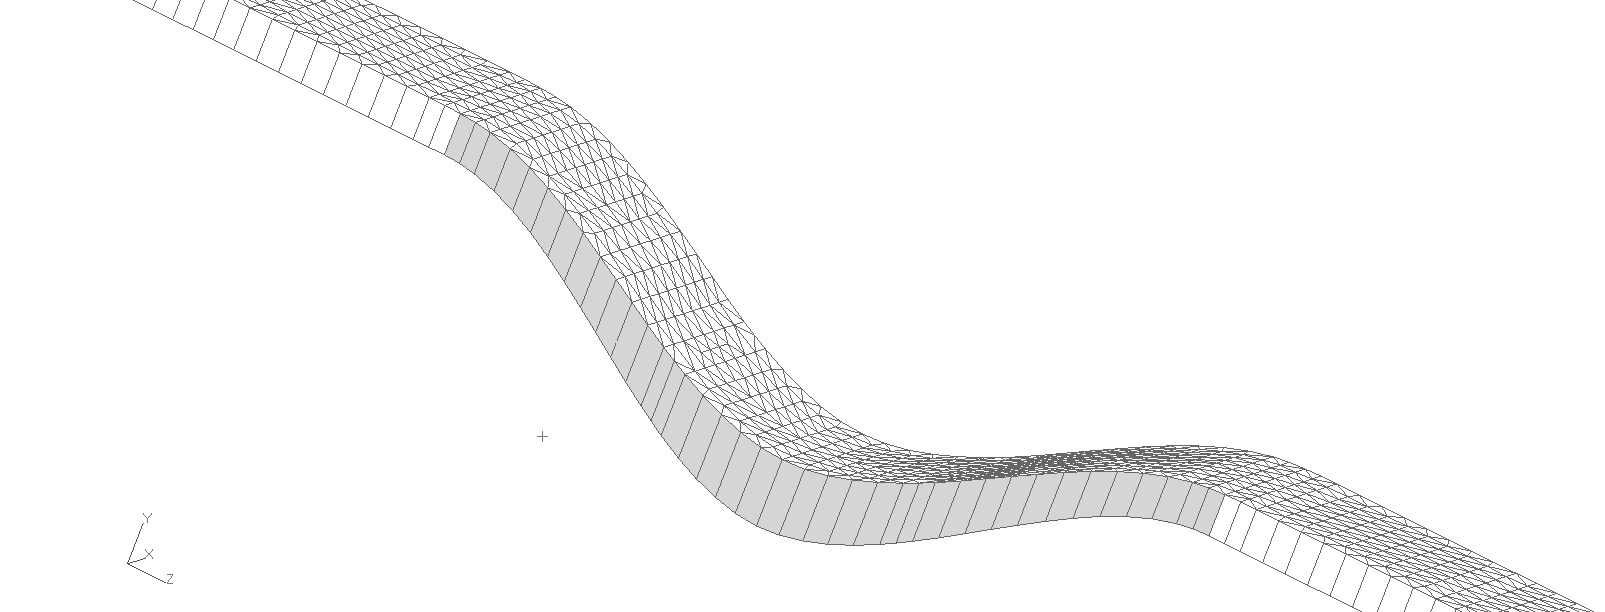
\includegraphics[width=0.9\textwidth]{simplifiedCentroplan}
\caption{Упрощенная МКЭ-модель центроплана}
\label{fig:simplifiedCentroplanMKE}
\end{figure}

Использование в МКЭ-расчете такой упрощенной модели позволяет значительно ускорить процесс прочностного параметрического анализа при тех же вычислительных мощностях. Так, в упрощенной модели используется $\approx10000$ конечных элементов, в то время как в МКЭ-модели полного БПЛА используется $\approx270000$ конечных элементов.

Как было сказано выше, рассматриваемая модель определяется двумя базовыми параметрами: координатой нижней точки сечения относительно базовой горизонтали БПЛА $y_\text{отн}$ и строительной высотой сечения в плоскости симметрии самолета $h_\text{стр}$. В качестве кривых, описывающих нижнюю и верхнюю поверхность кессона выбраны кубические сплайны, построенные через найденные исходя из выбранных параметров точки. Производные сплайнов в точках стыка фюзеляжа с крылом ($z=2.45\text{м}$) и в плоскости симметрии самолета ($z=0\text{м}$) приняты равными нулю. Пример модельного сечения центроплана в плоскости YZ со значениями параметров $h_\text{стр}=0.4\text{м}$, $y_\text{отн} = -1.4\text{м}$ приведен на Рис.\ref{fig:KessSectionExample}.

\begin{figure}[ht]
\centering
\def\svgwidth{\textwidth}
%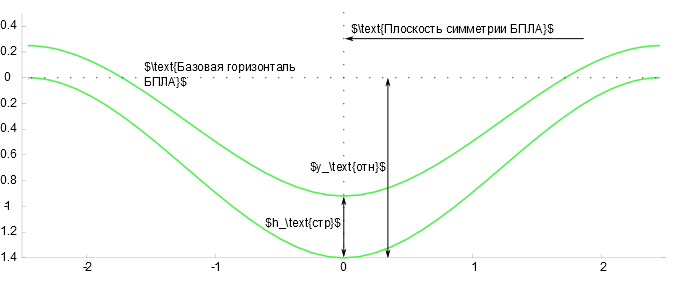
\includegraphics[width=1\textwidth]{KessSectionExample}
\input{figures/KessSectionExample.pdf_tex}
\caption{Пример формируемого параметрически поперечного сечения центроплана}
\label{fig:KessSectionExample}
\end{figure}


%\section{Оптимизация геометрических параметров сечения центроплана}
\subsection{Постановка задачи}
В ходе работы было проведено исследование зависимости веса центроплана от его параметров с учетом критерия неразрушения конструкции при заданных нагрузках. Для этого была решена следующая модельная задача.

\subsection{Постановка модельной задачи}
Имеется упрощенная модель центроплана -- короб переменного прямоугольного сечения с перегородками. На него передаются нагрузки посредством приложения аэродинамических нагрузок на модель крыла -- короб постоянного прямоугольного сечения. Для модели центроплана имеются два параметра: относительная координата нижней точки сечения и строительная высота в плоскости симметрии самолета. Было выбрано 42 пары параметров, для каждой пары проведена оптимизация сечения с целью удовлетворения требований прочности конструкции, а именно: среднее напряжение в каждой панели не должно превышать допускаемого напряжения, равного $35\text{кг}/\text{мм}^2$. Оптимизация проводилась алгоритмом $\sigma/\sigma$ для каждой панели. Итоговые результаты вычислений приведены в таблице \ref{tab:KessOptimBigTable} и на Рис.\ref{fig:Optimization3dplot}

\tabulinesep = 1mm
\definecolor{lightgray}{gray}{0.9}
\begin{table}[H]
\captionsetup{justification=centering}
\caption{Зависимость площади панелей центроплана и веса кессона от параметров центроплана}
%\rowcolors{2}{}{lightgray}
\begin{tabu}to \linewidth{|c|*4{X[m c]|}*4{X[m c]|}}
\hline
\multirow{2}{*}[-1.1ex]{N} & \multicolumn{4}{c|}{Вес кессона~[кг]} & \multicolumn{4}{c|}{Площадь панелей центроплана~[$\text{м}^2$]} \\ \cline{2-9}
& Верхние панели & Нижние панели & Боковые стенки & $\Sigma$ & Верхние панели & Нижние панели & Боковые стенки & $\Sigma$ \\
\hline
\taburowcolors {lightgray .. white}
1 & 297.182 & 294.551 & 12.561 & 604.294 & 2.730 & 2.730 & 4.000 & 9.520\\ \hline
2 & 225.261 & 237.378 & 27.672 & 490.313 & 2.730 & 2.740 & 5.210 & 10.720\\ \hline
3 & 190.080 & 222.327 & 49.159 & 461.564 & 2.730 & 2.760 & 5.820 & 11.340\\ \hline
4 & 161.544 & 211.467 & 65.963 & 438.972 & 2.730 & 2.760 & 6.450 & 11.950\\ \hline
5 & 146.581 & 199.989 & 66.844 & 413.415 & 2.730 & 2.780 & 7.090 & 12.590\\ \hline
6 & 134.746 & 191.293 & 70.912 & 396.952 & 2.730 & 2.800 & 7.640 & 13.200\\ \hline
7 & 350.816 & 374.021 & 47.679 & 772.515 & 2.910 & 2.910 & 4.000 & 9.850\\ \hline
8 & 253.752 & 259.311 & 53.180 & 566.245 & 2.910 & 2.850 & 5.210 & 10.990\\ \hline
9 & 213.881 & 226.655 & 57.618 & 498.154 & 2.910 & 2.830 & 5.840 & 11.570\\ \hline
10 & 188.442 & 205.603 & 62.047 & 456.092 & 2.910 & 2.810 & 6.450 & 12.150\\ \hline
11 & 174.466 & 196.192 & 66.506 & 437.164 & 2.910 & 2.780 & 7.090 & 12.770\\ \hline
12 & 154.328 & 195.919 & 70.963 & 421.210 & 2.910 & 2.770 & 7.680 & 13.350\\ \hline
13 & 363.681 & 391.414 & 48.862 & 803.953 & 3.010 & 3.000 & 4.000 & 10.000\\ \hline
14 & 258.118 & 275.555 & 53.209 & 586.883 & 3.010 & 2.930 & 5.230 & 11.160\\ \hline
15 & 225.322 & 238.220 & 57.604 & 521.145 & 3.010 & 2.890 & 5.820 & 11.720\\ \hline
16 & 201.612 & 214.755 & 62.046 & 478.413 & 3.010 & 2.860 & 6.440 & 12.310\\ \hline
17 & 171.877 & 203.370 & 66.418 & 441.665 & 3.010 & 2.840 & 7.050 & 12.900\\ \hline
18 & 163.553 & 201.207 & 70.912 & 435.673 & 3.010 & 2.820 & 7.660 & 13.480\\ \hline
19 & 380.079 & 398.521 & 49.032 & 827.631 & 3.050 & 3.050 & 4.000 & 10.110\\ \hline
20 & 267.143 & 279.590 & 53.134 & 599.866 & 3.050 & 2.980 & 5.210 & 11.240\\ \hline
21 & 231.158 & 238.954 & 57.667 & 527.779 & 3.050 & 2.930 & 5.820 & 11.820\\ \hline
22 & 197.327 & 218.001 & 62.040 & 477.368 & 3.050 & 2.910 & 6.410 & 12.390\\ \hline
23 & 191.553 & 205.935 & 66.481 & 463.971 & 3.050 & 2.870 & 7.070 & 12.980\\ \hline
24 & 158.352 & 203.948 & 70.897 & 433.199 & 3.050 & 2.850 & 7.660 & 13.560\\ \hline
25 & 383.525 & 410.374 & 50.351 & 844.249 & 3.110 & 3.110 & 4.000 & 10.210\\ \hline
26 & 279.228 & 288.331 & 53.186 & 620.745 & 3.110 & 3.030 & 5.210 & 11.350\\ \hline
27 & 233.614 & 249.500 & 57.583 & 540.696 & 3.110 & 2.990 & 5.820 & 11.910\\ \hline
28 & 213.922 & 221.683 & 62.125 & 497.728 & 3.110 & 2.950 & 6.450 & 12.500\\ \hline
29 & 180.457 & 210.067 & 66.523 & 457.046 & 3.110 & 2.920 & 7.070 & 13.070\\ \hline
30 & 167.492 & 205.426 & 71.001 & 443.918 & 3.110 & 2.880 & 7.640 & 13.660\\ \hline
31 & 401.418 & 424.040 & 50.413 & 875.868 & 3.160 & 3.160 & 4.000 & 10.330\\ \hline
32 & 285.115 & 297.451 & 53.649 & 636.214 & 3.160 & 3.070 & 5.230 & 11.470\\ \hline
33 & 251.131 & 255.015 & 57.656 & 563.801 & 3.160 & 3.040 & 5.860 & 12.030\\ \hline
34 & 212.049 & 229.543 & 62.067 & 503.658 & 3.160 & 3.000 & 6.450 & 12.610\\ \hline
35 & 191.030 & 215.968 & 66.550 & 473.548 & 3.160 & 2.970 & 7.070 & 13.170\\ \hline
36 & 170.765 & 209.184 & 70.962 & 450.912 & 3.160 & 2.920 & 7.660 & 13.740\\ \hline
37 & 431.880 & 451.562 & 51.974 & 935.418 & 3.230 & 3.230 & 4.000 & 10.440\\ \hline
38 & 291.199 & 306.178 & 54.263 & 651.640 & 3.230 & 3.130 & 5.210 & 11.560\\ \hline
39 & 253.054 & 265.073 & 57.593 & 575.719 & 3.230 & 3.090 & 5.820 & 12.140\\ \hline
40 & 222.782 & 233.403 & 61.948 & 518.132 & 3.230 & 3.050 & 6.400 & 12.700\\ \hline
41 & 197.192 & 218.301 & 66.423 & 481.917 & 3.230 & 3.020 & 7.030 & 13.270\\ \hline
42 & 175.591 & 210.828 & 70.877 & 457.295 & 3.230 & 2.970 & 7.660 & 13.840\\ \hline

\end{tabu}

\label{tab:KessOptimBigTable}
\end{table}


\tabulinesep = 1mm
\definecolor{lightgray}{gray}{0.9}
\begin{table}[H]
\captionsetup{justification=centering}
\caption{Зависимость площади панелей центроплана и веса кессона от параметров центроплана относительно варианта с прямым кессоном}
%\rowcolors{2}{}{lightgray}
\begin{tabu}to \linewidth{|c|*4{X[m c]|}*4{X[m c]|}}
\hline
\multirow{2}{*}[-1.1ex]{N} & \multicolumn{4}{c|}{Вес кессона} & \multicolumn{4}{c|}{Площадь панелей центроплана} \\ \cline{2-9}
& Верхние панели & Нижние панели & Боковые стенки & $\Sigma$ & Верхние панели & Нижние панели & Боковые стенки & $\Sigma$ \\
\hline
\taburowcolors {lightgray .. white}
1 & 0.492 & 0.487 & 0.021 & 1.000 & 0.287 & 0.287 & 0.420 & 1.000\\ \hline
2 & 0.373 & 0.393 & 0.046 & 0.811 & 0.287 & 0.288 & 0.547 & 1.126\\ \hline
3 & 0.315 & 0.368 & 0.081 & 0.764 & 0.287 & 0.290 & 0.611 & 1.191\\ \hline
4 & 0.267 & 0.350 & 0.109 & 0.726 & 0.287 & 0.290 & 0.678 & 1.255\\ \hline
5 & 0.243 & 0.331 & 0.111 & 0.684 & 0.287 & 0.292 & 0.745 & 1.322\\ \hline
6 & 0.223 & 0.317 & 0.117 & 0.657 & 0.287 & 0.294 & 0.803 & 1.387\\ \hline
7 & 0.581 & 0.619 & 0.079 & 1.278 & 0.306 & 0.306 & 0.420 & 1.035\\ \hline
8 & 0.420 & 0.429 & 0.088 & 0.937 & 0.306 & 0.299 & 0.547 & 1.154\\ \hline
9 & 0.354 & 0.375 & 0.095 & 0.824 & 0.306 & 0.297 & 0.613 & 1.215\\ \hline
10 & 0.312 & 0.340 & 0.103 & 0.755 & 0.306 & 0.295 & 0.678 & 1.276\\ \hline
11 & 0.289 & 0.325 & 0.110 & 0.723 & 0.306 & 0.292 & 0.745 & 1.341\\ \hline
12 & 0.255 & 0.324 & 0.117 & 0.697 & 0.306 & 0.291 & 0.807 & 1.402\\ \hline
13 & 0.602 & 0.648 & 0.081 & 1.330 & 0.316 & 0.315 & 0.420 & 1.050\\ \hline
14 & 0.427 & 0.456 & 0.088 & 0.971 & 0.316 & 0.308 & 0.549 & 1.172\\ \hline
15 & 0.373 & 0.394 & 0.095 & 0.862 & 0.316 & 0.304 & 0.611 & 1.231\\ \hline
16 & 0.334 & 0.355 & 0.103 & 0.792 & 0.316 & 0.300 & 0.676 & 1.293\\ \hline
17 & 0.284 & 0.337 & 0.110 & 0.731 & 0.316 & 0.298 & 0.741 & 1.355\\ \hline
18 & 0.271 & 0.333 & 0.117 & 0.721 & 0.316 & 0.296 & 0.805 & 1.416\\ \hline
19 & 0.629 & 0.659 & 0.081 & 1.370 & 0.320 & 0.320 & 0.420 & 1.062\\ \hline
20 & 0.442 & 0.463 & 0.088 & 0.993 & 0.320 & 0.313 & 0.547 & 1.181\\ \hline
21 & 0.383 & 0.395 & 0.095 & 0.873 & 0.320 & 0.308 & 0.611 & 1.242\\ \hline
22 & 0.327 & 0.361 & 0.103 & 0.790 & 0.320 & 0.306 & 0.673 & 1.301\\ \hline
23 & 0.317 & 0.341 & 0.110 & 0.768 & 0.320 & 0.301 & 0.743 & 1.363\\ \hline
24 & 0.262 & 0.337 & 0.117 & 0.717 & 0.320 & 0.299 & 0.805 & 1.424\\ \hline
25 & 0.635 & 0.679 & 0.083 & 1.397 & 0.327 & 0.327 & 0.420 & 1.072\\ \hline
26 & 0.462 & 0.477 & 0.088 & 1.027 & 0.327 & 0.318 & 0.547 & 1.192\\ \hline
27 & 0.387 & 0.413 & 0.095 & 0.895 & 0.327 & 0.314 & 0.611 & 1.251\\ \hline
28 & 0.354 & 0.367 & 0.103 & 0.824 & 0.327 & 0.310 & 0.678 & 1.313\\ \hline
29 & 0.299 & 0.348 & 0.110 & 0.756 & 0.327 & 0.307 & 0.743 & 1.373\\ \hline
30 & 0.277 & 0.340 & 0.117 & 0.735 & 0.327 & 0.303 & 0.803 & 1.435\\ \hline
31 & 0.664 & 0.702 & 0.083 & 1.449 & 0.332 & 0.332 & 0.420 & 1.085\\ \hline
32 & 0.472 & 0.492 & 0.089 & 1.053 & 0.332 & 0.322 & 0.549 & 1.205\\ \hline
33 & 0.416 & 0.422 & 0.095 & 0.933 & 0.332 & 0.319 & 0.616 & 1.264\\ \hline
34 & 0.351 & 0.380 & 0.103 & 0.833 & 0.332 & 0.315 & 0.678 & 1.325\\ \hline
35 & 0.316 & 0.357 & 0.110 & 0.784 & 0.332 & 0.312 & 0.743 & 1.383\\ \hline
36 & 0.283 & 0.346 & 0.117 & 0.746 & 0.332 & 0.307 & 0.805 & 1.443\\ \hline
37 & 0.715 & 0.747 & 0.086 & 1.548 & 0.339 & 0.339 & 0.420 & 1.097\\ \hline
38 & 0.482 & 0.507 & 0.090 & 1.078 & 0.339 & 0.329 & 0.547 & 1.214\\ \hline
39 & 0.419 & 0.439 & 0.095 & 0.953 & 0.339 & 0.325 & 0.611 & 1.275\\ \hline
40 & 0.369 & 0.386 & 0.103 & 0.857 & 0.339 & 0.320 & 0.672 & 1.334\\ \hline
41 & 0.326 & 0.361 & 0.110 & 0.797 & 0.339 & 0.317 & 0.738 & 1.394\\ \hline
42 & 0.291 & 0.349 & 0.117 & 0.757 & 0.339 & 0.312 & 0.805 & 1.454\\ \hline

\end{tabu}

\label{tab:KessOptimBigTable}
\end{table}

\begin{landscape}
\begin{figure}[ht]
\captionsetup{justification=centering}
\caption{Зависимость веса кессона от параметров центроплана}
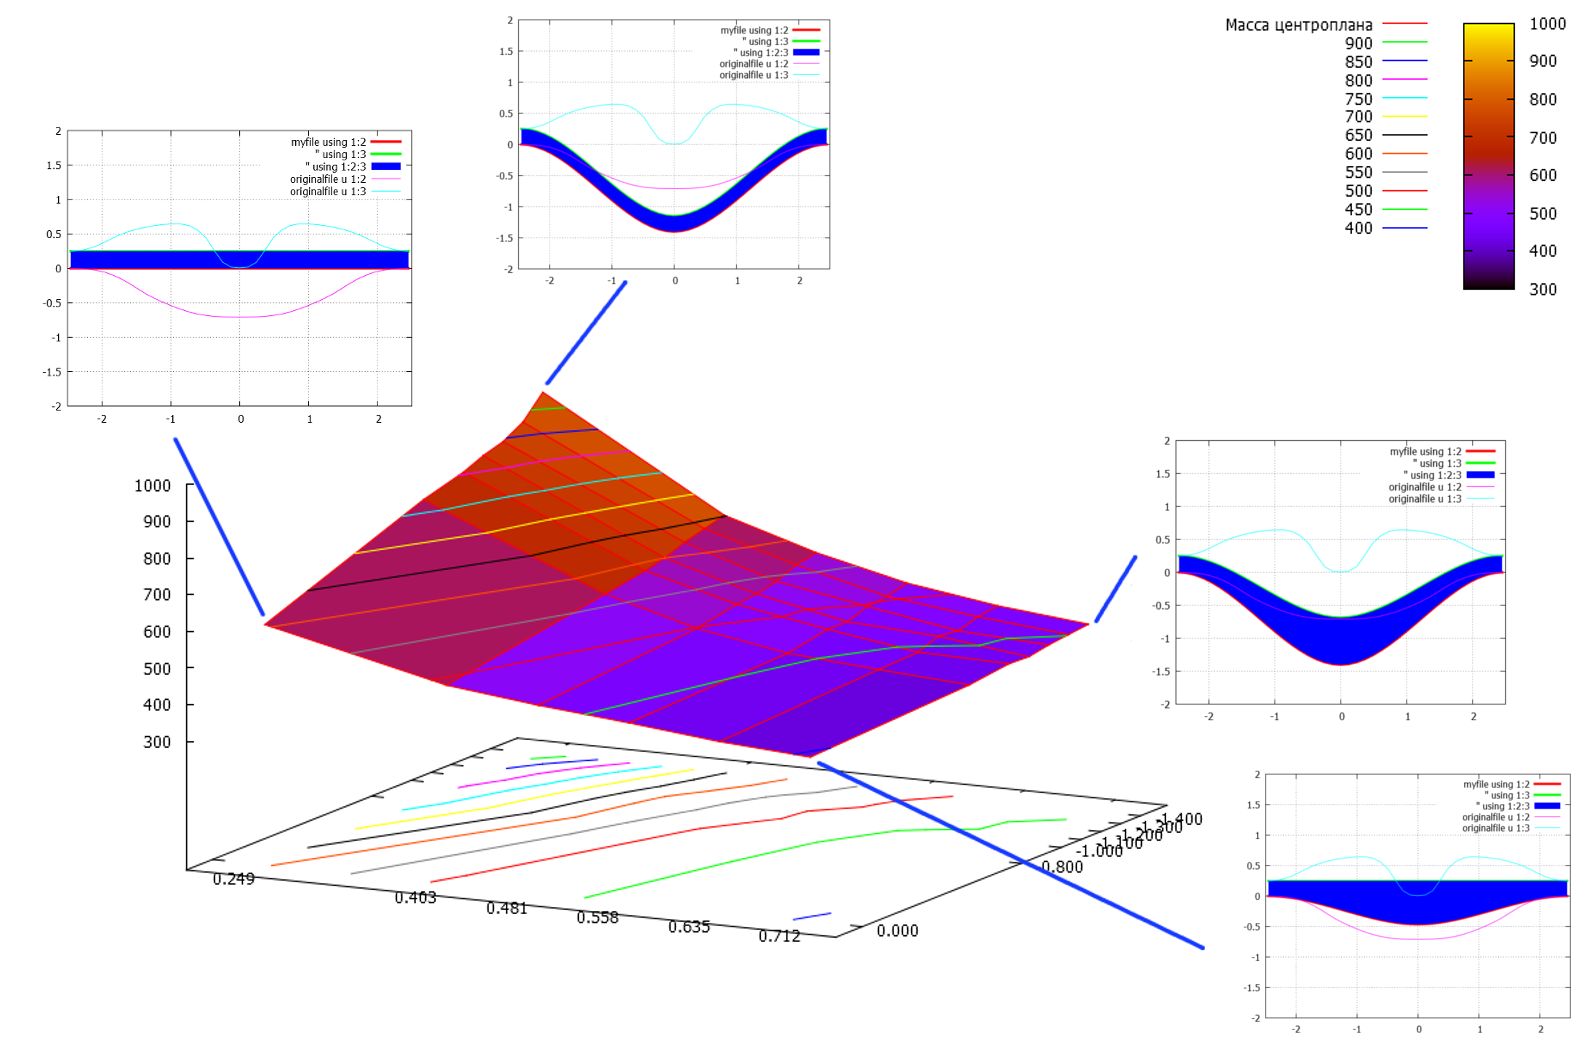
\includegraphics[height=0.9\textwidth]{Optimization3dplot}
\label{fig:Optimization3dplot}
\end{figure}
\end{landscape}



\section{Расчет параметрической модели}
\label{sec:calculationOfModel}
Для проведения параметрического расчета были выбраны 42 пары значений параметров. Для каждой пары значений была проведена оптимизация толщин панелей модели с целью удовлетворения требованиям прочности конструкции. Оптимизация была проведена путем многократных нахождения запаса прочности для каждой панели (стенки отсека) с последующим делением толщины панели на полученное значение (так называемый алгоритм $\sigma/\sigma$). Итоговые результаты вычислений приведены в таблицах \ref{tab:KessTableNormedComparison}, \ref{tab:KessOptimBigTableNormed} и на Рис.\ref{fig:Optimization3dplot} (серым цветом на изображениях сечений показано оригинальное сечение кессона в гипотетической модели БПЛА-ЦАГИ, зеленым - сечение в параметрической модели)  

%%%%%%%%%%%%%%%%%%%%%%%%%%%%%%%%%%


\tabulinesep = 1mm
\definecolor{lightgray}{gray}{0.9}
\begin{table}[ht]
    \fontsize{11pt}{12pt}\selectfont
\captionsetup{justification=centering}
\caption{Зависимость веса кессона от параметров центроплана относительно варианта с прямым кессоном}
%\rowcolors{2}{}{lightgray}
\begin{tabu}to \linewidth{|>{\columncolor{lightgray}}c|*8{X[m c]|}}
\hline
%\taburowcolors {lightgray .. white}
\rowcolor{lightgray}
$h_\text{стр} \setminus y_\text{отн}$		&	0.000	&	-0.800	&	-1.000	&	-1.100	&	-1.200	&	-1.300	&	-1.400  \\ \hline 
0.249	&	1.000	&	1.278	&	1.330	&	1.370	&	1.397	&	1.449	&	1.548	\\ \hline
0.403	&	0.811	&	0.937	&	0.971	&	0.993	&	1.027	&	1.053	&	1.078	\\ \hline
0.481	&	0.764	&	0.824	&	0.862	&	0.873	&	0.895	&	0.933	&	0.953	\\ \hline
0.558	&	0.726	&	0.755	&	0.792	&	0.790	&	0.824	&	0.833	&	0.857	\\ \hline
0.635	&	0.684	&	0.723	&	0.731	&	0.768	&	0.756	&	0.784	&	0.797	\\ \hline
0.712	&	0.657	&	0.697	&	0.721	&	0.717	&	0.735	&	0.746	&	0.757	\\ \hline
\end{tabu}

\label{tab:KessTableNormedComparison}
\end{table}

%\tabulinesep = 1mm
%\definecolor{lightgray}{gray}{0.9}
%\begin{table}[H]
%
%
%    \fontsize{12pt}{14pt}\selectfont
%\captionsetup{justification=centering}
%\caption{Зависимость площади панелей центроплана и веса кессона от параметров центроплана (данные надо пересчитывать)}
%%\rowcolors{2}{}{lightgray}
%\begin{tabu}to \linewidth{|c|*4{X[m c]|}*4{X[m c]|}}
%\hline
%\multirow{2}{*}[-1.1ex]{N} & \multicolumn{4}{c|}{Вес кессона~[кг]} & \multicolumn{4}{c|}{Площадь панелей центроплана~[$\text{м}^2$]} \\ \cline{2-9}
%& Верхние панели & Нижние панели & Боковые стенки & $\Sigma$ & Верхние панели & Нижние панели & Боковые стенки & $\Sigma$ \\
%\hline
%\taburowcolors {lightgray .. white}
%1 & 297.182 & 294.551 & 12.561 & 604.294 & 2.730 & 2.730 & 4.000 & 9.520\\ \hline
2 & 225.261 & 237.378 & 27.672 & 490.313 & 2.730 & 2.740 & 5.210 & 10.720\\ \hline
3 & 190.080 & 222.327 & 49.159 & 461.564 & 2.730 & 2.760 & 5.820 & 11.340\\ \hline
4 & 161.544 & 211.467 & 65.963 & 438.972 & 2.730 & 2.760 & 6.450 & 11.950\\ \hline
5 & 146.581 & 199.989 & 66.844 & 413.415 & 2.730 & 2.780 & 7.090 & 12.590\\ \hline
6 & 134.746 & 191.293 & 70.912 & 396.952 & 2.730 & 2.800 & 7.640 & 13.200\\ \hline
7 & 350.816 & 374.021 & 47.679 & 772.515 & 2.910 & 2.910 & 4.000 & 9.850\\ \hline
8 & 253.752 & 259.311 & 53.180 & 566.245 & 2.910 & 2.850 & 5.210 & 10.990\\ \hline
9 & 213.881 & 226.655 & 57.618 & 498.154 & 2.910 & 2.830 & 5.840 & 11.570\\ \hline
10 & 188.442 & 205.603 & 62.047 & 456.092 & 2.910 & 2.810 & 6.450 & 12.150\\ \hline
11 & 174.466 & 196.192 & 66.506 & 437.164 & 2.910 & 2.780 & 7.090 & 12.770\\ \hline
12 & 154.328 & 195.919 & 70.963 & 421.210 & 2.910 & 2.770 & 7.680 & 13.350\\ \hline
13 & 363.681 & 391.414 & 48.862 & 803.953 & 3.010 & 3.000 & 4.000 & 10.000\\ \hline
14 & 258.118 & 275.555 & 53.209 & 586.883 & 3.010 & 2.930 & 5.230 & 11.160\\ \hline
15 & 225.322 & 238.220 & 57.604 & 521.145 & 3.010 & 2.890 & 5.820 & 11.720\\ \hline
16 & 201.612 & 214.755 & 62.046 & 478.413 & 3.010 & 2.860 & 6.440 & 12.310\\ \hline
17 & 171.877 & 203.370 & 66.418 & 441.665 & 3.010 & 2.840 & 7.050 & 12.900\\ \hline
18 & 163.553 & 201.207 & 70.912 & 435.673 & 3.010 & 2.820 & 7.660 & 13.480\\ \hline
19 & 380.079 & 398.521 & 49.032 & 827.631 & 3.050 & 3.050 & 4.000 & 10.110\\ \hline
20 & 267.143 & 279.590 & 53.134 & 599.866 & 3.050 & 2.980 & 5.210 & 11.240\\ \hline
21 & 231.158 & 238.954 & 57.667 & 527.779 & 3.050 & 2.930 & 5.820 & 11.820\\ \hline
22 & 197.327 & 218.001 & 62.040 & 477.368 & 3.050 & 2.910 & 6.410 & 12.390\\ \hline
23 & 191.553 & 205.935 & 66.481 & 463.971 & 3.050 & 2.870 & 7.070 & 12.980\\ \hline
24 & 158.352 & 203.948 & 70.897 & 433.199 & 3.050 & 2.850 & 7.660 & 13.560\\ \hline
25 & 383.525 & 410.374 & 50.351 & 844.249 & 3.110 & 3.110 & 4.000 & 10.210\\ \hline
26 & 279.228 & 288.331 & 53.186 & 620.745 & 3.110 & 3.030 & 5.210 & 11.350\\ \hline
27 & 233.614 & 249.500 & 57.583 & 540.696 & 3.110 & 2.990 & 5.820 & 11.910\\ \hline
28 & 213.922 & 221.683 & 62.125 & 497.728 & 3.110 & 2.950 & 6.450 & 12.500\\ \hline
29 & 180.457 & 210.067 & 66.523 & 457.046 & 3.110 & 2.920 & 7.070 & 13.070\\ \hline
30 & 167.492 & 205.426 & 71.001 & 443.918 & 3.110 & 2.880 & 7.640 & 13.660\\ \hline
31 & 401.418 & 424.040 & 50.413 & 875.868 & 3.160 & 3.160 & 4.000 & 10.330\\ \hline
32 & 285.115 & 297.451 & 53.649 & 636.214 & 3.160 & 3.070 & 5.230 & 11.470\\ \hline
33 & 251.131 & 255.015 & 57.656 & 563.801 & 3.160 & 3.040 & 5.860 & 12.030\\ \hline
34 & 212.049 & 229.543 & 62.067 & 503.658 & 3.160 & 3.000 & 6.450 & 12.610\\ \hline
35 & 191.030 & 215.968 & 66.550 & 473.548 & 3.160 & 2.970 & 7.070 & 13.170\\ \hline
36 & 170.765 & 209.184 & 70.962 & 450.912 & 3.160 & 2.920 & 7.660 & 13.740\\ \hline
37 & 431.880 & 451.562 & 51.974 & 935.418 & 3.230 & 3.230 & 4.000 & 10.440\\ \hline
38 & 291.199 & 306.178 & 54.263 & 651.640 & 3.230 & 3.130 & 5.210 & 11.560\\ \hline
39 & 253.054 & 265.073 & 57.593 & 575.719 & 3.230 & 3.090 & 5.820 & 12.140\\ \hline
40 & 222.782 & 233.403 & 61.948 & 518.132 & 3.230 & 3.050 & 6.400 & 12.700\\ \hline
41 & 197.192 & 218.301 & 66.423 & 481.917 & 3.230 & 3.020 & 7.030 & 13.270\\ \hline
42 & 175.591 & 210.828 & 70.877 & 457.295 & 3.230 & 2.970 & 7.660 & 13.840\\ \hline
%\end{tabu}
%
%\label{tab:KessOptimBigTable}
%\end{table}

%%%%%%%%%%%%%%%%%%%%%%%%%%%%%%%%%

\tabulinesep = 1mm
\definecolor{lightgray}{gray}{0.9}
\begin{table}[ht]
    \fontsize{11pt}{12pt}\selectfont
\captionsetup{justification=centering}
\caption{Зависимость площади панелей центроплана и веса кессона от параметров центроплана относительно варианта с прямым кессоном}
%\rowcolors{2}{}{lightgray}
\begin{tabu}to \linewidth{|c|c|*4{X[m c]|}*4{X[m c]|}}
\hline
\multirow{2}{*}[-1.1ex]{$y_\text{отн}$} & \multirow{2}{*}[-1.1ex]{$h_\text{стр}$} & \multicolumn{4}{c|}{Вес кессона} & \multicolumn{4}{c|}{Площадь панелей центроплана} \\ \cline{3-9}
& & Верхние панели & Нижние панели & Боковые стенки & $\Sigma$ & Верхние панели & Нижние панели & Боковые стенки & $\Sigma$ \\
\hline
\taburowcolors {lightgray .. white}
1 & 0.492 & 0.487 & 0.021 & 1.000 & 0.287 & 0.287 & 0.420 & 1.000\\ \hline
2 & 0.373 & 0.393 & 0.046 & 0.811 & 0.287 & 0.288 & 0.547 & 1.126\\ \hline
3 & 0.315 & 0.368 & 0.081 & 0.764 & 0.287 & 0.290 & 0.611 & 1.191\\ \hline
4 & 0.267 & 0.350 & 0.109 & 0.726 & 0.287 & 0.290 & 0.678 & 1.255\\ \hline
5 & 0.243 & 0.331 & 0.111 & 0.684 & 0.287 & 0.292 & 0.745 & 1.322\\ \hline
6 & 0.223 & 0.317 & 0.117 & 0.657 & 0.287 & 0.294 & 0.803 & 1.387\\ \hline
7 & 0.581 & 0.619 & 0.079 & 1.278 & 0.306 & 0.306 & 0.420 & 1.035\\ \hline
8 & 0.420 & 0.429 & 0.088 & 0.937 & 0.306 & 0.299 & 0.547 & 1.154\\ \hline
9 & 0.354 & 0.375 & 0.095 & 0.824 & 0.306 & 0.297 & 0.613 & 1.215\\ \hline
10 & 0.312 & 0.340 & 0.103 & 0.755 & 0.306 & 0.295 & 0.678 & 1.276\\ \hline
11 & 0.289 & 0.325 & 0.110 & 0.723 & 0.306 & 0.292 & 0.745 & 1.341\\ \hline
12 & 0.255 & 0.324 & 0.117 & 0.697 & 0.306 & 0.291 & 0.807 & 1.402\\ \hline
13 & 0.602 & 0.648 & 0.081 & 1.330 & 0.316 & 0.315 & 0.420 & 1.050\\ \hline
14 & 0.427 & 0.456 & 0.088 & 0.971 & 0.316 & 0.308 & 0.549 & 1.172\\ \hline
15 & 0.373 & 0.394 & 0.095 & 0.862 & 0.316 & 0.304 & 0.611 & 1.231\\ \hline
16 & 0.334 & 0.355 & 0.103 & 0.792 & 0.316 & 0.300 & 0.676 & 1.293\\ \hline
17 & 0.284 & 0.337 & 0.110 & 0.731 & 0.316 & 0.298 & 0.741 & 1.355\\ \hline
18 & 0.271 & 0.333 & 0.117 & 0.721 & 0.316 & 0.296 & 0.805 & 1.416\\ \hline
19 & 0.629 & 0.659 & 0.081 & 1.370 & 0.320 & 0.320 & 0.420 & 1.062\\ \hline
20 & 0.442 & 0.463 & 0.088 & 0.993 & 0.320 & 0.313 & 0.547 & 1.181\\ \hline
21 & 0.383 & 0.395 & 0.095 & 0.873 & 0.320 & 0.308 & 0.611 & 1.242\\ \hline
22 & 0.327 & 0.361 & 0.103 & 0.790 & 0.320 & 0.306 & 0.673 & 1.301\\ \hline
23 & 0.317 & 0.341 & 0.110 & 0.768 & 0.320 & 0.301 & 0.743 & 1.363\\ \hline
24 & 0.262 & 0.337 & 0.117 & 0.717 & 0.320 & 0.299 & 0.805 & 1.424\\ \hline
25 & 0.635 & 0.679 & 0.083 & 1.397 & 0.327 & 0.327 & 0.420 & 1.072\\ \hline
26 & 0.462 & 0.477 & 0.088 & 1.027 & 0.327 & 0.318 & 0.547 & 1.192\\ \hline
27 & 0.387 & 0.413 & 0.095 & 0.895 & 0.327 & 0.314 & 0.611 & 1.251\\ \hline
28 & 0.354 & 0.367 & 0.103 & 0.824 & 0.327 & 0.310 & 0.678 & 1.313\\ \hline
29 & 0.299 & 0.348 & 0.110 & 0.756 & 0.327 & 0.307 & 0.743 & 1.373\\ \hline
30 & 0.277 & 0.340 & 0.117 & 0.735 & 0.327 & 0.303 & 0.803 & 1.435\\ \hline
31 & 0.664 & 0.702 & 0.083 & 1.449 & 0.332 & 0.332 & 0.420 & 1.085\\ \hline
32 & 0.472 & 0.492 & 0.089 & 1.053 & 0.332 & 0.322 & 0.549 & 1.205\\ \hline
33 & 0.416 & 0.422 & 0.095 & 0.933 & 0.332 & 0.319 & 0.616 & 1.264\\ \hline
34 & 0.351 & 0.380 & 0.103 & 0.833 & 0.332 & 0.315 & 0.678 & 1.325\\ \hline
35 & 0.316 & 0.357 & 0.110 & 0.784 & 0.332 & 0.312 & 0.743 & 1.383\\ \hline
36 & 0.283 & 0.346 & 0.117 & 0.746 & 0.332 & 0.307 & 0.805 & 1.443\\ \hline
37 & 0.715 & 0.747 & 0.086 & 1.548 & 0.339 & 0.339 & 0.420 & 1.097\\ \hline
38 & 0.482 & 0.507 & 0.090 & 1.078 & 0.339 & 0.329 & 0.547 & 1.214\\ \hline
39 & 0.419 & 0.439 & 0.095 & 0.953 & 0.339 & 0.325 & 0.611 & 1.275\\ \hline
40 & 0.369 & 0.386 & 0.103 & 0.857 & 0.339 & 0.320 & 0.672 & 1.334\\ \hline
41 & 0.326 & 0.361 & 0.110 & 0.797 & 0.339 & 0.317 & 0.738 & 1.394\\ \hline
42 & 0.291 & 0.349 & 0.117 & 0.757 & 0.339 & 0.312 & 0.805 & 1.454\\ \hline

\end{tabu}

\label{tab:KessOptimBigTableNormed}
\end{table}




%%%%%%%%%%%%%%%%%%%%%%%%%%%%%%%%%%%%%%%%

%\begin{landscape}
\begin{figure}[ht]
\captionsetup{justification=centering}
\caption{Зависимость веса кессона от параметров центроплана (данные надо пересчитывать)}
%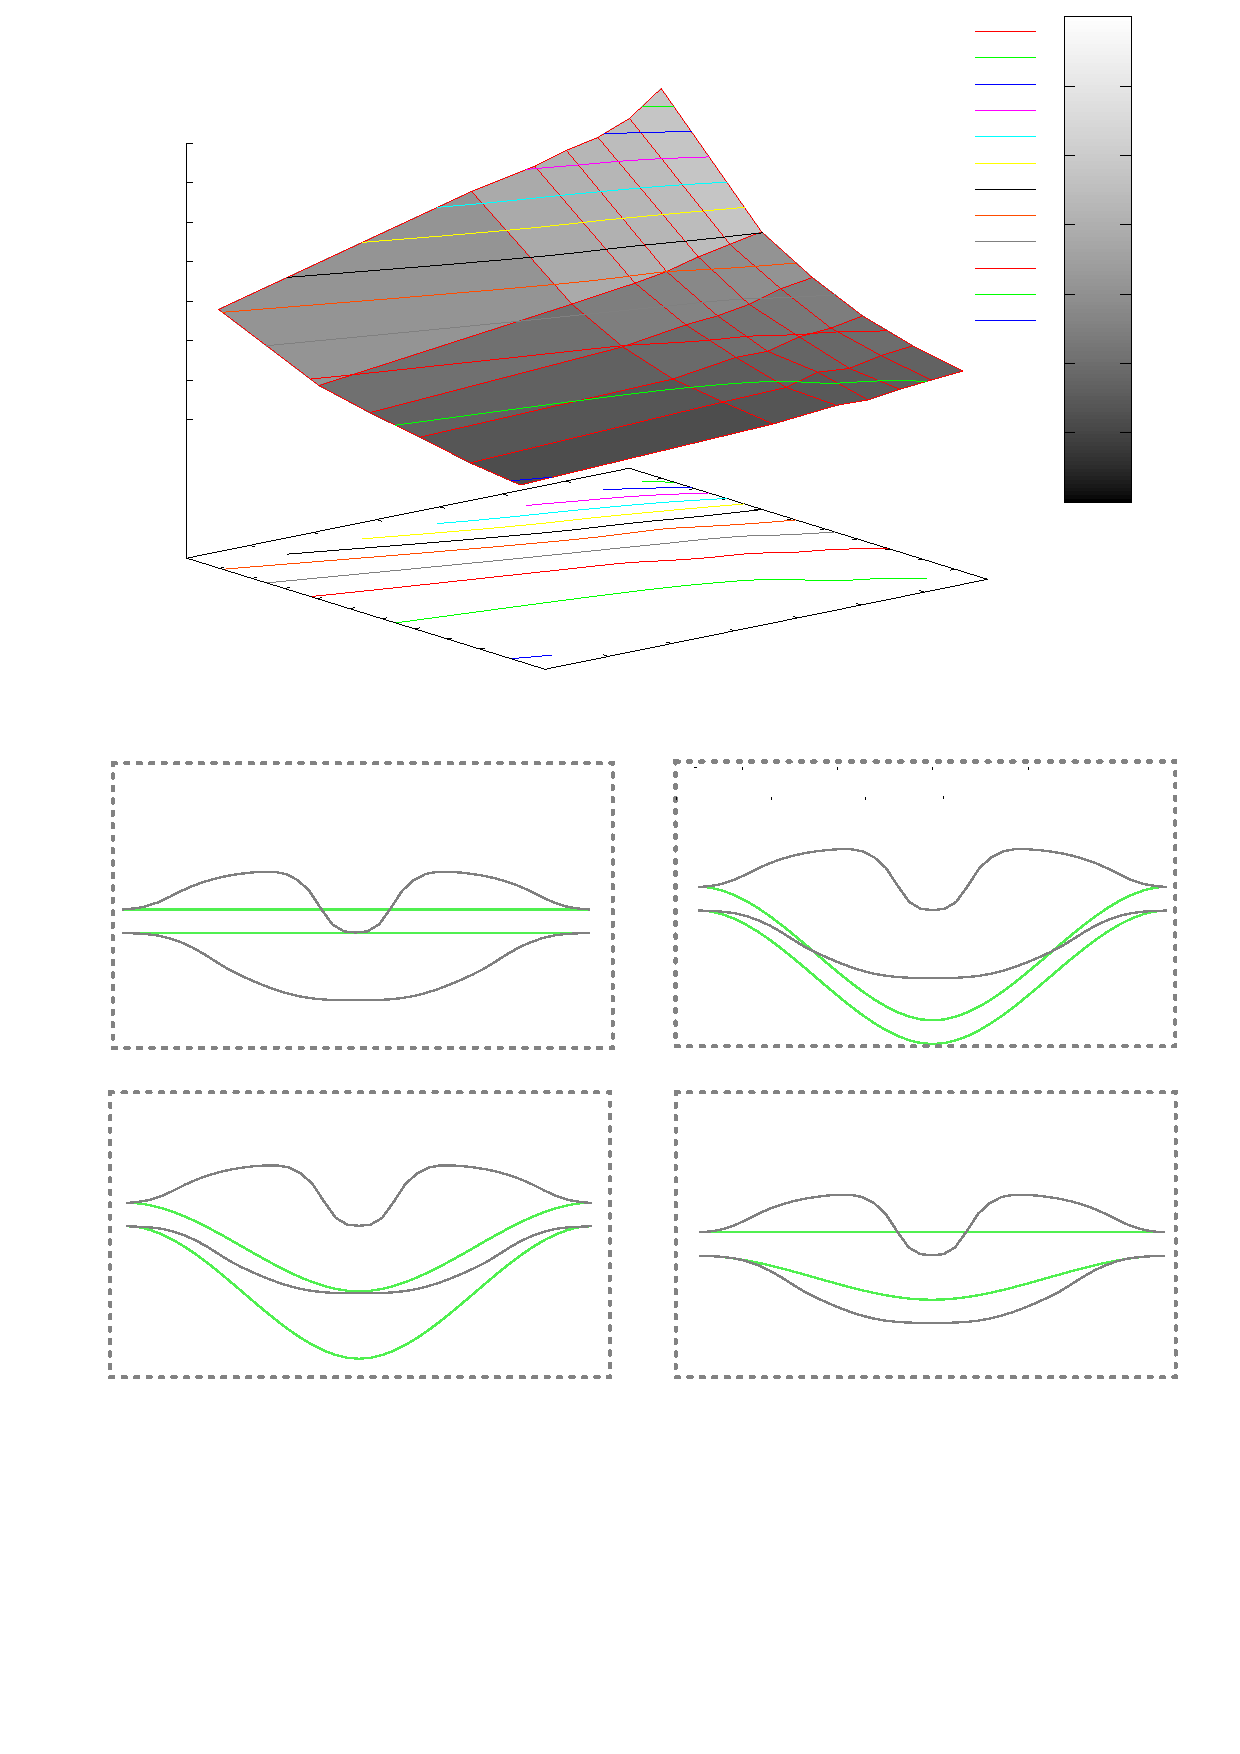
\includegraphics[width=0.9\textwidth]{3dplot_with_sections}
\def\svgwidth{\textwidth}
\input{figures/3dplot_with_sections.pdf_tex}
\label{fig:Optimization3dplot}
\end{figure}
%\end{landscape}

Как показывают полученные данные, оптимальная из рассмотренных форма сечения определяется следующими значениями параметров: $y_\text{отн} = 0\text{м},\quad h_\text{стр}=1.4\text{м}$. Вид данного сечения представлен на Рис.\ref{fig:optimalSection}. Значение веса кессона центроплана для данного сечения равно 397кг. 
 
\chapter{Выбор рациональной конструкции}
Как было отмечено в разделе \ref{sec:ndsResults}, одним из проблемных с точки зрения прочности мест конструкции гипотетического БПЛА является элемент конструкции, обеспечивающий основное крепление хвостовой части к центропланом. В целях нахождения конструкции гипотетического БПЛА минимального веса в работе был проведен сравнительный анализ различных вариантов исполнения данного элемента. Для проведения анализа были выбраны три варианта конструкции, представленные на схемах на Рис.\ref{fig:variants_plain} и изображениях МКЭ-моделей на Рис.\ref{fig:variants_mke}. Для анализа была использована модель, описанная в разделе \ref{sec:creationOfOneModel} и две модели, созданные на её основе. Все три модели были адаптированы с учетом выводов, которые будут получены в разделе \ref{sec:optimalMKESize}.  

\begin{figure}[H]
\centering
\captionsetup{justification=centering}
\begin{subfigure}[b]{0.32\textwidth}
\centering
	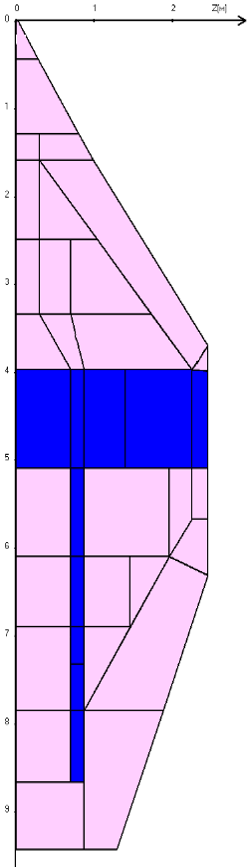
\includegraphics[width=0.3\textwidth]{variants/1_plain}
	\caption{Вариант 1}
\end{subfigure}
\hspace{\fill}
\begin{subfigure}[b]{0.32\textwidth}
\centering
	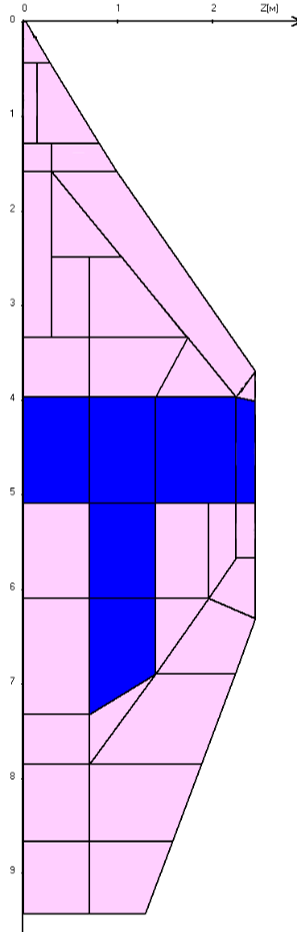
\includegraphics[width=0.3\textwidth]{variants/2_plain}
	\caption{Вариант 2}
\end{subfigure}
\hspace{\fill}
\begin{subfigure}[b]{0.32\textwidth}
\centering
	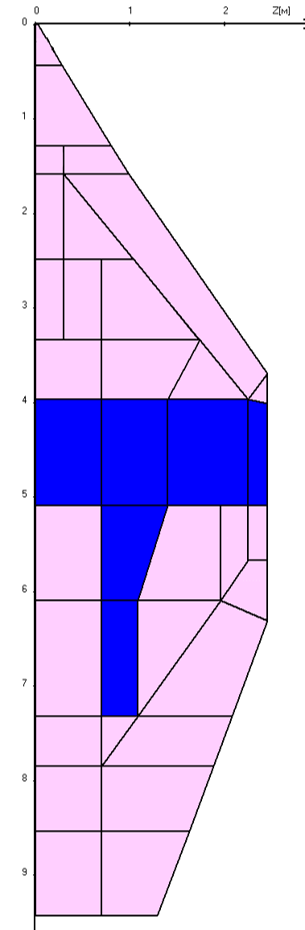
\includegraphics[width=0.3\textwidth]{variants/3_plain}
	\caption{Вариант 3}
\end{subfigure}
\hspace{\fill}
\caption{Схематичные изображения центроплана и соединительной конструкции на виде ``в плане'' половины фюзеляжа }
\label{fig:variants_plain}
\end{figure}	


\begin{figure}[H]
\centering
\begin{subfigure}[b]{0.32\textwidth}
	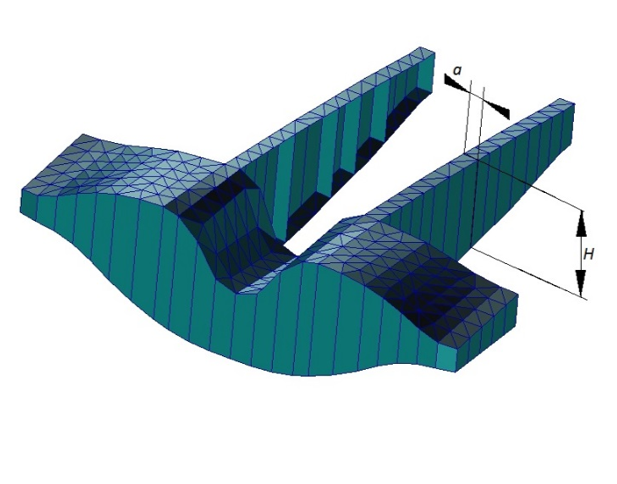
\includegraphics[width=\textwidth]{variants/1_mke}		\caption{Вариант 1}
	\label{fig:variants_mke:1}
\end{subfigure}
\hspace{\fill}
\begin{subfigure}[b]{0.32\textwidth}
	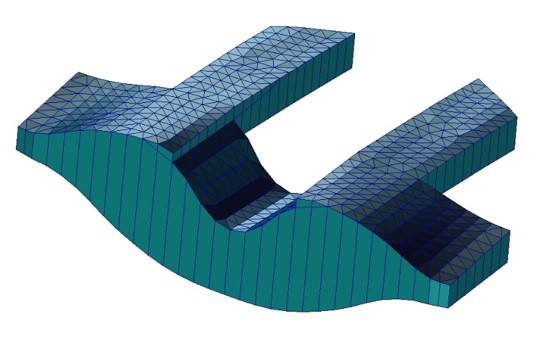
\includegraphics[width=\textwidth]{variants/2_mke}
		\caption{Вариант 2}
		\label{fig:variants_mke:2}
\end{subfigure}
\hspace{\fill}
\begin{subfigure}[b]{0.32\textwidth}
	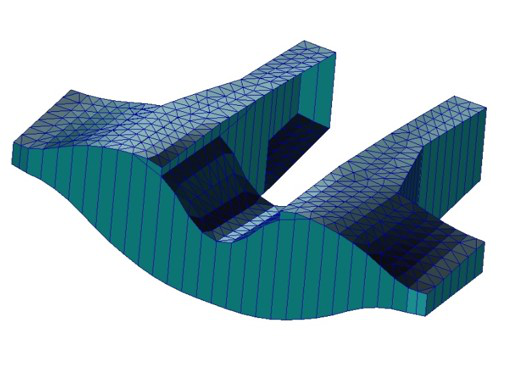
\includegraphics[width=\textwidth]{variants/3_mke}
		\caption{Вариант 3}
		\label{fig:variants_mke:3}
\end{subfigure}
\hspace{\fill}
\caption{Виды МКЭ-моделей центроплана и соединительного элемента}
\label{fig:variants_mke}
\end{figure}	



\section{Подбор оптимальной дискретности модели}
\label{sec:optimalMKESize}

В целях обеспечения точности расчета было проведено исследование зависимости 
НДС гипотетической модели БПЛА, представленной в разделе \ref{sec:creationOfOneModel} (именуемой далее базовой моделью), от максимального характерного размера конечных элементов, используемых в модели. 

С помощью программного комплекса ``Conver'' на основе базовой модели было построено 7 моделей БПЛА, отличающихся лишь максимальным размером конечных элементов, используемых при построении модели. Для сравнительного анализа моделей были выбраны четыре точки, в которых, в соответствии с результатами, полученными в разделе \ref{sec:ndsResults}, обнаруживаются наибольшие напряжения. Путем расчета полученных моделей с помощью программного продукта MSC.Nastran были получены величины напряжений в этих четырех точках для каждой модели.

%Нужно пересчитывать график

\begin{figure}[ht]
\centering
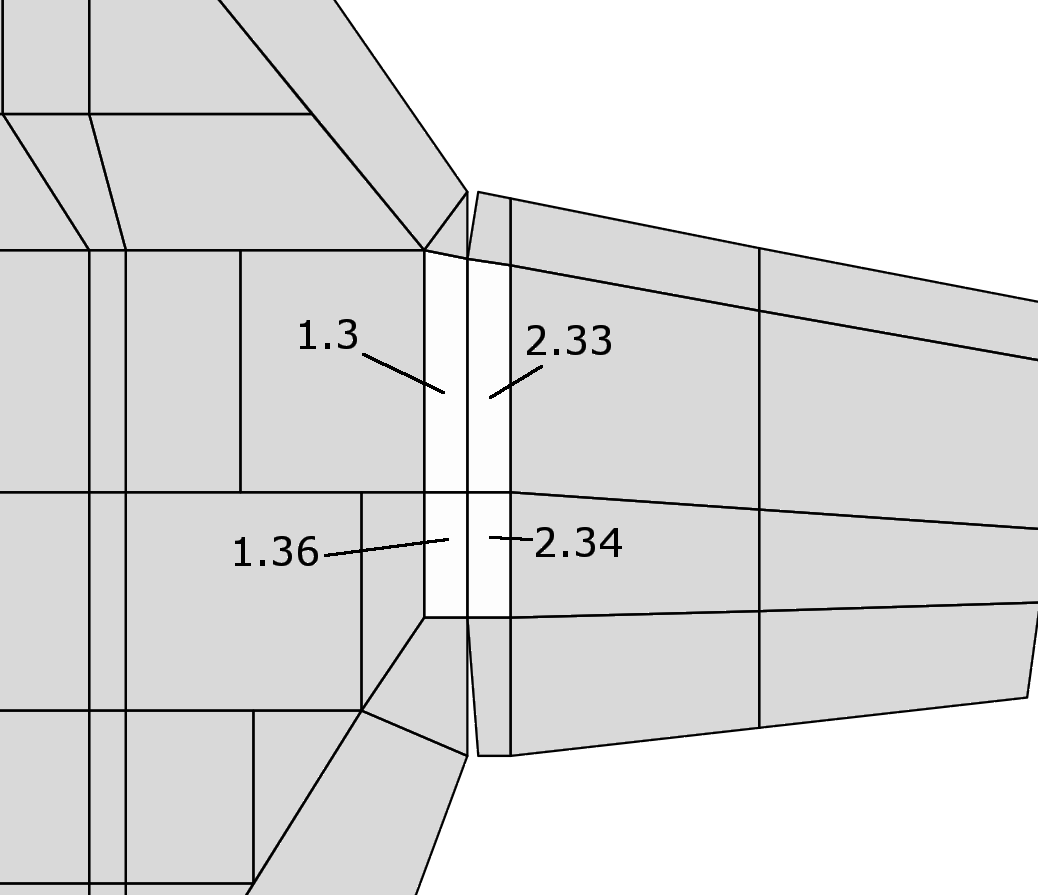
\includegraphics[width=0.5\textwidth]{RootOfWingWithSelectedPartsBW}
\caption{Схематичное изображение вида сверху в месте стыка правого крыла и фюзеляжа}
\label{fig:WingRootPlain}
\end{figure}


\begin{figure}[H]
\captionsetup{justification=centering}
\centering
	\begin{subfigure}[b]{0.8\textwidth}
	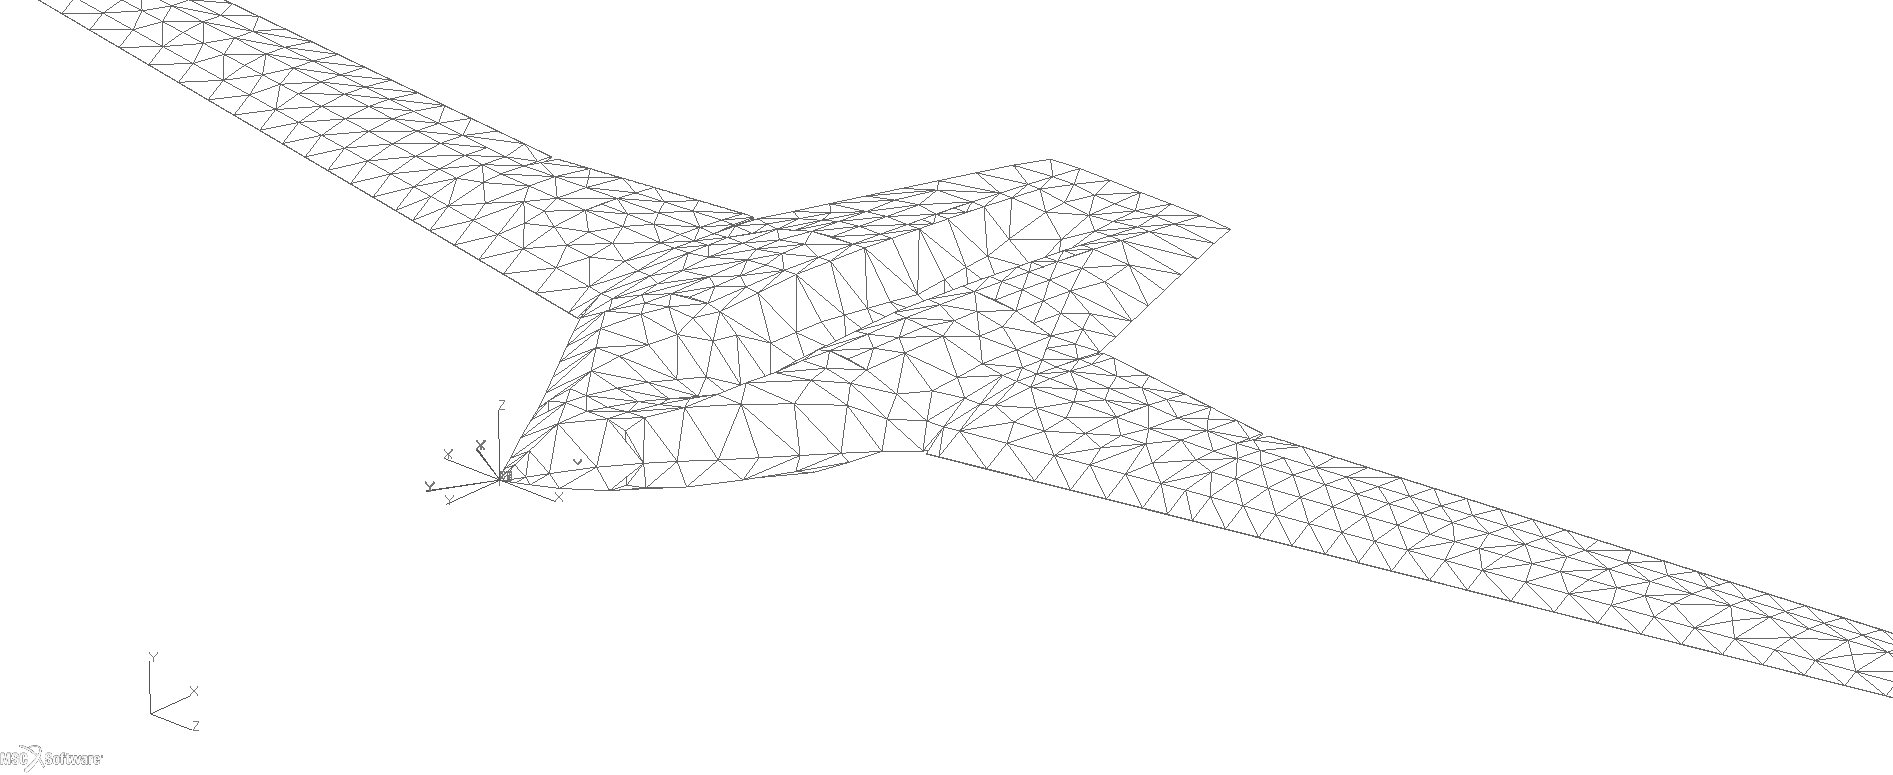
\includegraphics[width=0.98\textwidth]{discreteness/0_4}
	\caption{$L_\text{КЭ} = 0.4см$}
	\label{fig:discr:0_4}
	\end{subfigure}
	\begin{subfigure}[b]{0.8\textwidth}
	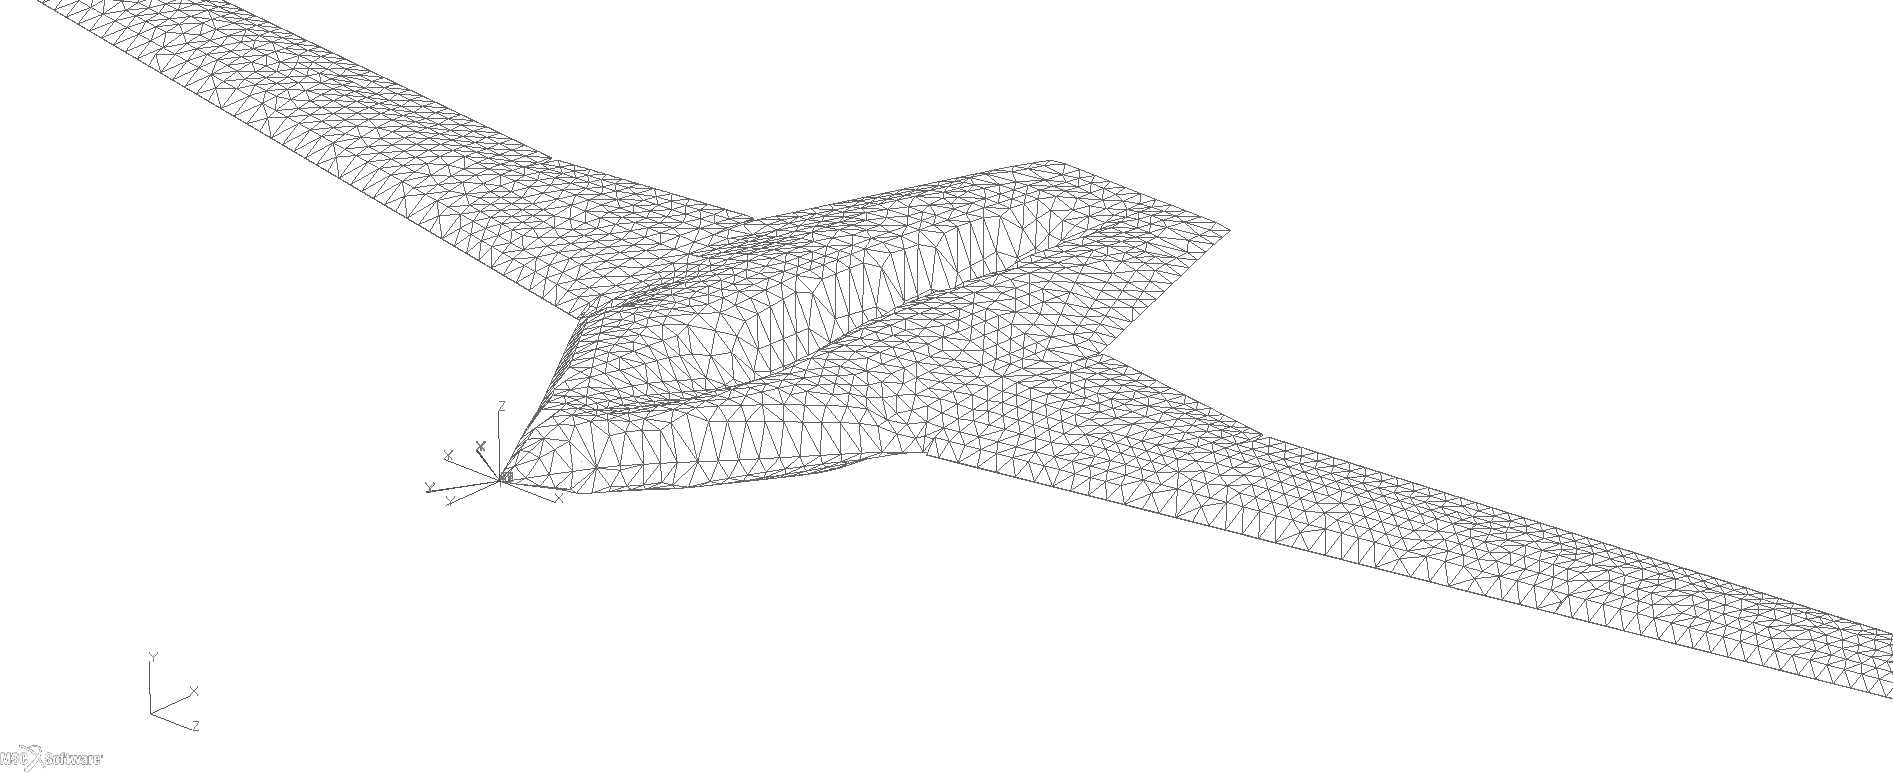
\includegraphics[width=0.98\textwidth]{discreteness/0_2}
	\caption{$L_\text{КЭ} = 0.2см$}
	\label{fig:discr:0_2}
	\end{subfigure}
	\begin{subfigure}[b]{0.8\textwidth}
	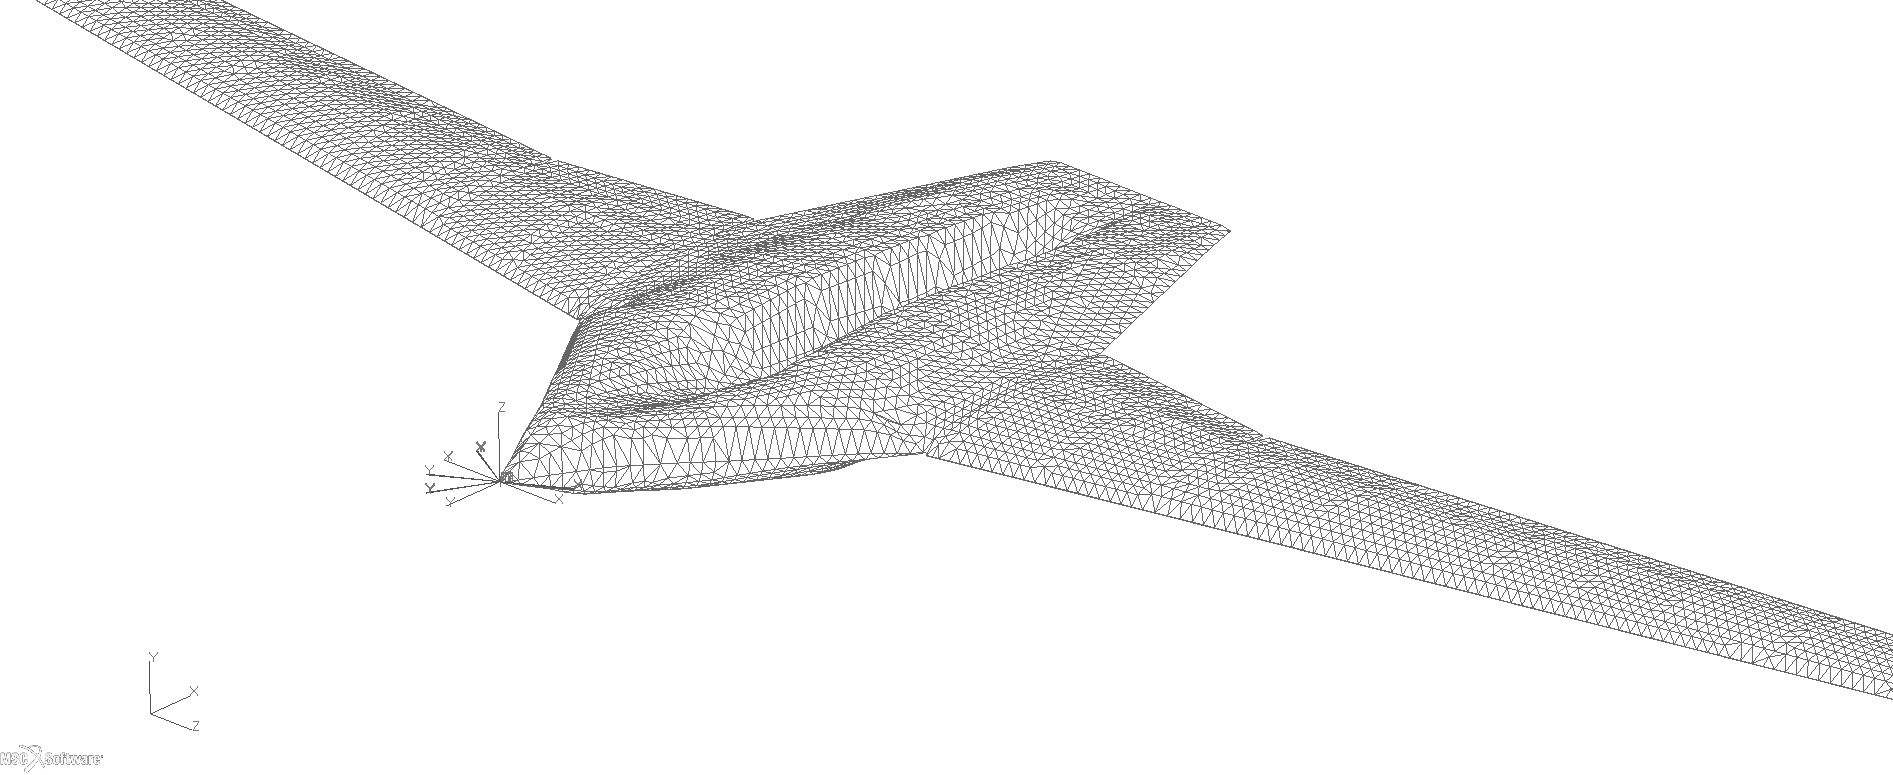
\includegraphics[width=0.98\textwidth]{discreteness/0_13}
	\caption{$L_\text{КЭ} = 0.13см$}
	\label{fig:discr:0_13}
	\end{subfigure}
\label{fig:discreteness}
\caption{Изображения МКЭ-моделей гипотетического БПЛА, построенных с использованием различных характерных размеров конечного элемента}
\end{figure}





На Рис.\ref{fig:stressToDiscreteness} представлена зависимость найденых эквивалентных напряжений (напряжений по Мизесу) в выбранных точках от максимального размера конечного элемента, используемого при построении модели. 

\begin{figure}[H]
\centering
%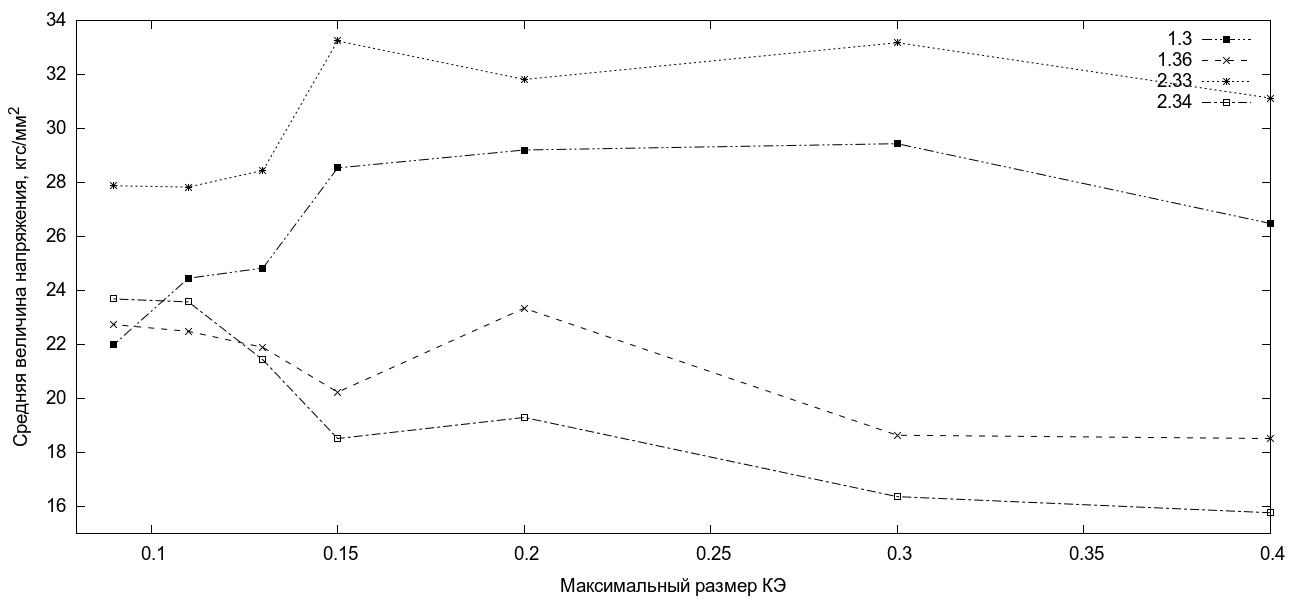
\includegraphics[width=0.8\textwidth]{StressToDiscretenessPlot}
\def\svgwidth{\textwidth}
% GNUPLOT: LaTeX picture with Postscript
\begingroup
  \makeatletter
  \providecommand\color[2][]{%
    \GenericError{(gnuplot) \space\space\space\@spaces}{%
      Package color not loaded in conjunction with
      terminal option `colourtext'%
    }{See the gnuplot documentation for explanation.%
    }{Either use 'blacktext' in gnuplot or load the package
      color.sty in LaTeX.}%
    \renewcommand\color[2][]{}%
  }%
  \providecommand\includegraphics[2][]{%
    \GenericError{(gnuplot) \space\space\space\@spaces}{%
      Package graphicx or graphics not loaded%
    }{See the gnuplot documentation for explanation.%
    }{The gnuplot epslatex terminal needs graphicx.sty or graphics.sty.}%
    \renewcommand\includegraphics[2][]{}%
  }%
  \providecommand\rotatebox[2]{#2}%
  \@ifundefined{ifGPcolor}{%
    \newif\ifGPcolor
    \GPcolorfalse
  }{}%
  \@ifundefined{ifGPblacktext}{%
    \newif\ifGPblacktext
    \GPblacktexttrue
  }{}%
  % define a \g@addto@macro without @ in the name:
  \let\gplgaddtomacro\g@addto@macro
  % define empty templates for all commands taking text:
  \gdef\gplbacktext{}%
  \gdef\gplfronttext{}%
  \makeatother
  \ifGPblacktext
    % no textcolor at all
    \def\colorrgb#1{}%
    \def\colorgray#1{}%
  \else
    % gray or color?
    \ifGPcolor
      \def\colorrgb#1{\color[rgb]{#1}}%
      \def\colorgray#1{\color[gray]{#1}}%
      \expandafter\def\csname LTw\endcsname{\color{white}}%
      \expandafter\def\csname LTb\endcsname{\color{black}}%
      \expandafter\def\csname LTa\endcsname{\color{black}}%
      \expandafter\def\csname LT0\endcsname{\color[rgb]{1,0,0}}%
      \expandafter\def\csname LT1\endcsname{\color[rgb]{0,1,0}}%
      \expandafter\def\csname LT2\endcsname{\color[rgb]{0,0,1}}%
      \expandafter\def\csname LT3\endcsname{\color[rgb]{1,0,1}}%
      \expandafter\def\csname LT4\endcsname{\color[rgb]{0,1,1}}%
      \expandafter\def\csname LT5\endcsname{\color[rgb]{1,1,0}}%
      \expandafter\def\csname LT6\endcsname{\color[rgb]{0,0,0}}%
      \expandafter\def\csname LT7\endcsname{\color[rgb]{1,0.3,0}}%
      \expandafter\def\csname LT8\endcsname{\color[rgb]{0.5,0.5,0.5}}%
    \else
      % gray
      \def\colorrgb#1{\color{black}}%
      \def\colorgray#1{\color[gray]{#1}}%
      \expandafter\def\csname LTw\endcsname{\color{white}}%
      \expandafter\def\csname LTb\endcsname{\color{black}}%
      \expandafter\def\csname LTa\endcsname{\color{black}}%
      \expandafter\def\csname LT0\endcsname{\color{black}}%
      \expandafter\def\csname LT1\endcsname{\color{black}}%
      \expandafter\def\csname LT2\endcsname{\color{black}}%
      \expandafter\def\csname LT3\endcsname{\color{black}}%
      \expandafter\def\csname LT4\endcsname{\color{black}}%
      \expandafter\def\csname LT5\endcsname{\color{black}}%
      \expandafter\def\csname LT6\endcsname{\color{black}}%
      \expandafter\def\csname LT7\endcsname{\color{black}}%
      \expandafter\def\csname LT8\endcsname{\color{black}}%
    \fi
  \fi
  \setlength{\unitlength}{0.0500bp}%
  \begin{picture}(8502.00,4534.00)%
    \gplgaddtomacro\gplbacktext{%
      \csname LTb\endcsname%
      \put(814,892){\makebox(0,0)[r]{\strut{} 16}}%
      \put(814,1267){\makebox(0,0)[r]{\strut{} 18}}%
      \put(814,1642){\makebox(0,0)[r]{\strut{} 20}}%
      \put(814,2017){\makebox(0,0)[r]{\strut{} 22}}%
      \put(814,2393){\makebox(0,0)[r]{\strut{} 24}}%
      \put(814,2768){\makebox(0,0)[r]{\strut{} 26}}%
      \put(814,3143){\makebox(0,0)[r]{\strut{} 28}}%
      \put(814,3518){\makebox(0,0)[r]{\strut{} 30}}%
      \put(814,3894){\makebox(0,0)[r]{\strut{} 32}}%
      \put(814,4269){\makebox(0,0)[r]{\strut{} 34}}%
      \put(1393,484){\makebox(0,0){\strut{} 0.1}}%
      \put(2512,484){\makebox(0,0){\strut{} 0.15}}%
      \put(3631,484){\makebox(0,0){\strut{} 0.2}}%
      \put(4749,484){\makebox(0,0){\strut{} 0.25}}%
      \put(5868,484){\makebox(0,0){\strut{} 0.3}}%
      \put(6986,484){\makebox(0,0){\strut{} 0.35}}%
      \put(8105,484){\makebox(0,0){\strut{} 0.4}}%
      \put(176,2486){\rotatebox{-270}{\makebox(0,0){\strut{}Средняя величина напряжения, $\text{кгс}/\text{мм}^2$}}}%
      \put(4525,154){\makebox(0,0){\strut{}Максимальный размер КЭ}}%
    }%
    \gplgaddtomacro\gplfronttext{%
      \csname LTb\endcsname%
      \put(7118,4096){\makebox(0,0)[r]{\strut{}$1.3$}}%
      \csname LTb\endcsname%
      \put(7118,3876){\makebox(0,0)[r]{\strut{}$1.36$}}%
      \csname LTb\endcsname%
      \put(7118,3656){\makebox(0,0)[r]{\strut{}$2.33$}}%
      \csname LTb\endcsname%
      \put(7118,3436){\makebox(0,0)[r]{\strut{}$2.34$}}%
    }%
    \gplbacktext
    \put(0,0){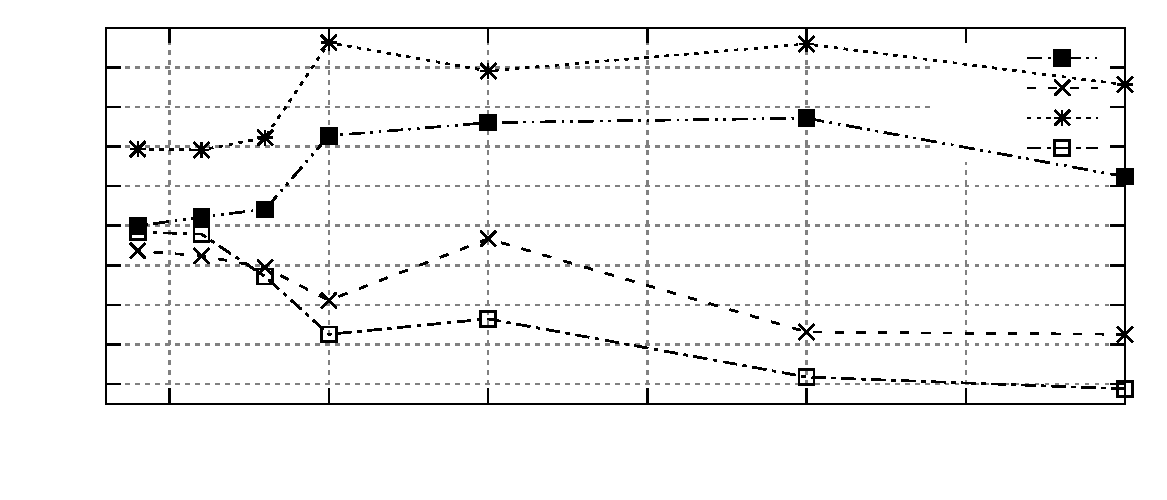
\includegraphics{StressToDiscreteness}}%
    \gplfronttext
  \end{picture}%
\endgroup

\caption{Зависимость напряжений в выбранных точках от максимальной величины КЭ, используемой в модели}
\label{fig:stressToDiscreteness}
\end{figure}


	

Исходя из полученных данных и с учетом зависимости трудоемкости процесса от максимального размера КЭ, была определена оптимальная для дальнейших параметрических исследований моделей гипотетического БПЛА величина конечного элемента, равная $0,11\text{м}$. 
%Ниже приведены картины НДС в месте стыка крыла с фюзеляжем при различных размерах конечного элемента. 


\section{Сравнение моделей}

Как было описано выше, в работе был проведен сравнительный анализ трех вариантов конструкции элемента, обеспечивающего крепление хвостовой части фюзеляжа к центроплану. Первый вариант представляет собой длинный узкий короб с несколькими перегородками (Рис.\ref{fig:variants_mke:1}). В первом варианте двигатель крепится в двух местах непосредственно к стенке короба. Данный вариант частично соответствует модельному варианту n стенок с $n = 4$, рассмотренному в разделе \ref{sec:pants}. Во втором варианте используется широкий плоский короб, частично расположенный над шассийной нишей (Рис.\ref{fig:variants_mke:2}). В данном варианте двигатель крепится к стенке короба и на боковое ребро короба. Третий вариант является промежуточным между первым и вторым и представляет собой широкий короб, соответствующий по высоте фюзеляжной части центроплана в месте их крепления (Рис.\ref{fig:variants_mke:3}). В данном варианте двигатель крепится аналогично второму варианту. 

В ходе сравнительного анализа моделей был проведен МКЭ-расчет созданных моделей с помощью программного продукта MSC.Nastran. В результате расчета были получены напряженно-деформированные состояния каждой из моделей. Ниже приведено сравнение весовых характеристик моделей. Нумерация моделей в таблице соответствует нумерации на рисунках \ref{fig:variants_plain} и \ref{fig:variants_mke}

\tabulinesep = 1mm
\definecolor{lightgray}{gray}{0.9}
\begin{table}[H]
\captionsetup{justification=centering}
\caption{Таблица весовых характеристик моделей}
\begin{tabu}to \linewidth{*4{|X[m c]}|}
\hline
\taburowcolors {lightgray .. white}
 & Вариант 1 & Вариант 2 & Вариант 3 \\ \hline
масса фюзеляжа & 850кг & 812кг  & 778кг \\ \hline
относительная масса фюзеляжа & $100\%$ & $95\%$ & $91,5\%$ \\ \hline
%масса обшивки & 489кг & 505кг  & 499кг \\ \hline
%масса подкрепляющего набора & 361кг & 307кг  & 277кг \\ \hline
\end{tabu}
\label{tab:variantsMasses}
\end{table}

Из полученных данных сделан вывод о том, что оптимальным по весовым характеристикам является использование третьего варианта конструкции.  


\chapter*{Выводы}

Сформированы основные базовые требования к проведению многодисциплинарного проектирования перспективной гипотетической конструкции БПЛА с крылом большого удлинения и криволинейной формой центроплана. 

Была обоснована необходимость:
\begin{itemize}
\item использования параметрической МКЭ-модели большой размерности всей конструкции БПЛА;
\item решения модельной задачи по определению зависимости веса конструкции БПЛА от геометрических параметров, определяющих форму искривленного центроплана;
\item выбора рациональной КСС корневой части кабины БПЛА в зоне крепления двигателя.
\end{itemize}

Построена параметрическая МКЭ-модель большой размерности гипотетической конструкции БПЛА для проведения проектировочных исследований по поиску рациональных проектных параметров конструкции, обеспечивающих минимальные весовые характеристики гипотетической конструкции БПЛА. 

Модель позволяет проводить исследования прочности конструкции гипотетического БПЛА как для металлических, так и для композиционных конструкционных материалов (в бакалаврской работе были рассмотрены только металлические варианты конструкции). При построении конечноэлементной модели исползовались коммерческие программные комплексы: patran, nastran, а также программные комплексы, разработанные в ЦАГИ: конвер, (Крючков) и (Фомин).
Проектировочная модель  включала свыше 30 базовых варьируемых параметров. 

Найдена рациональная размерность конечноэлементной модели с характерным размером конечного элемента, равным 0.11м, и количеством конечных элементов порядка $200000$. 

Валидационные исследования, проведенные в рамках параметрической МКЭ-модели, показали ее высокую точность при определении локальных параметров НДС, а также хорошее соответствие результатов с результатами, полученных на альтернативных моделях и МКЭ-модели конструкции БПЛА-ЦАГИ. 


Решена модельная задача по определению зависимости веса конструкции искривленного центроплана от базовых геометрических параметров, определяющих форму центроплана: максимальной строительной высоты центроплана и параметра, характеризующего кривизну центроплана (расстояние от средней горизонтали ЛА до нижней точки сечения). Получены рациональные значения базовых параметров, реализующие минимум веса конструкции центроплана. Соответствующие параметры равны: . Представлены результаты (весовые характеристики конструкции центроплана) для 42 комбинаций данных параметров, которые могут быть использованы в дальнейшем для решения многодисциплинарной проектировочной задачи с изменением геометрических параметров, формирующих внешние обводы. 

Аналогичное: проведены сравнительные весовые исследования трех альтернативных КСС гипотетической конструкции БПЛА с различными схемами организации крепления двигателя. Описать целиком. 
%в третью главу 
%\chapter{Проектировочное исследование}
\section{Создание конечно-элементной модели проектируемого самолета}

В ходе работы были исследованы вопросы построения проектировочной модели БПЛА с крылом большого удлинения и несущим фюзеляжем. При помощи программного комплекса ``Conver'' (см. раздел \ref{sec:Conver}), исходя из концептуальной модели, предложенной конструкторами, была создана МКЭ-модель проектируемого БПЛА с исключенной верхней частью воздухозаборника, не несущей в себе силовых элементов. 

\begin{figure}[ht]
\centering
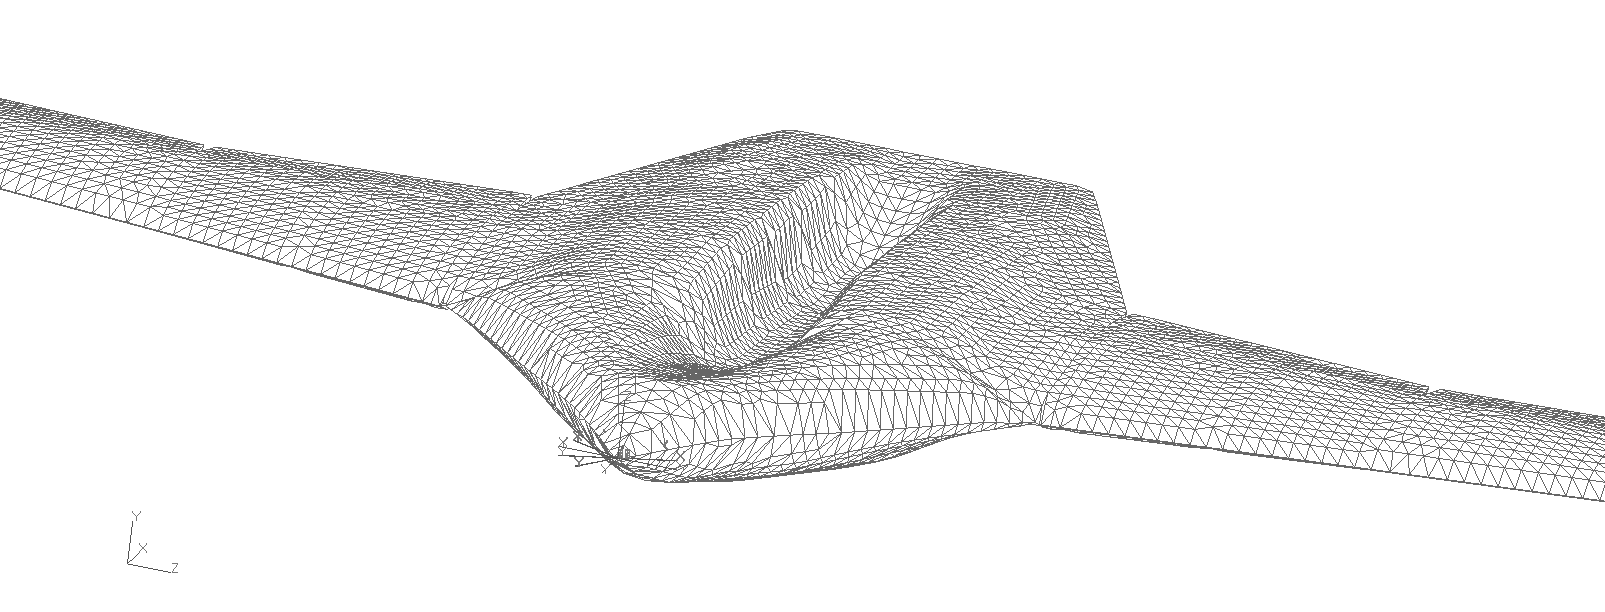
\includegraphics[width=0.8\textwidth]{BPLAfullModel}
\caption{МКЭ-модель проектируемого БПЛА без верхней части}
\label{fig:BPLAfullModel}
\end{figure}

\subsection{Подбор оптимальной дискретности модели}

В целях обеспечения точности расчета было проведено исследование зависимости напряженно-деформированного состояния самолета от максимального характерного размера конечных элементов, используемых в модели. 

С помощью программного комплекса ``Conver'' было построено 7 моделей самолета по одинаковой схеме с использованием различных размеров конечного элемента. Путем расчета моделей были определены средние величины напряжений для панелей и стенок в наиболее напряженных отсеках самолета (обозначены белым на  Рис.\ref{fig:WingRootPlain})

\begin{figure}[ht]
\centering
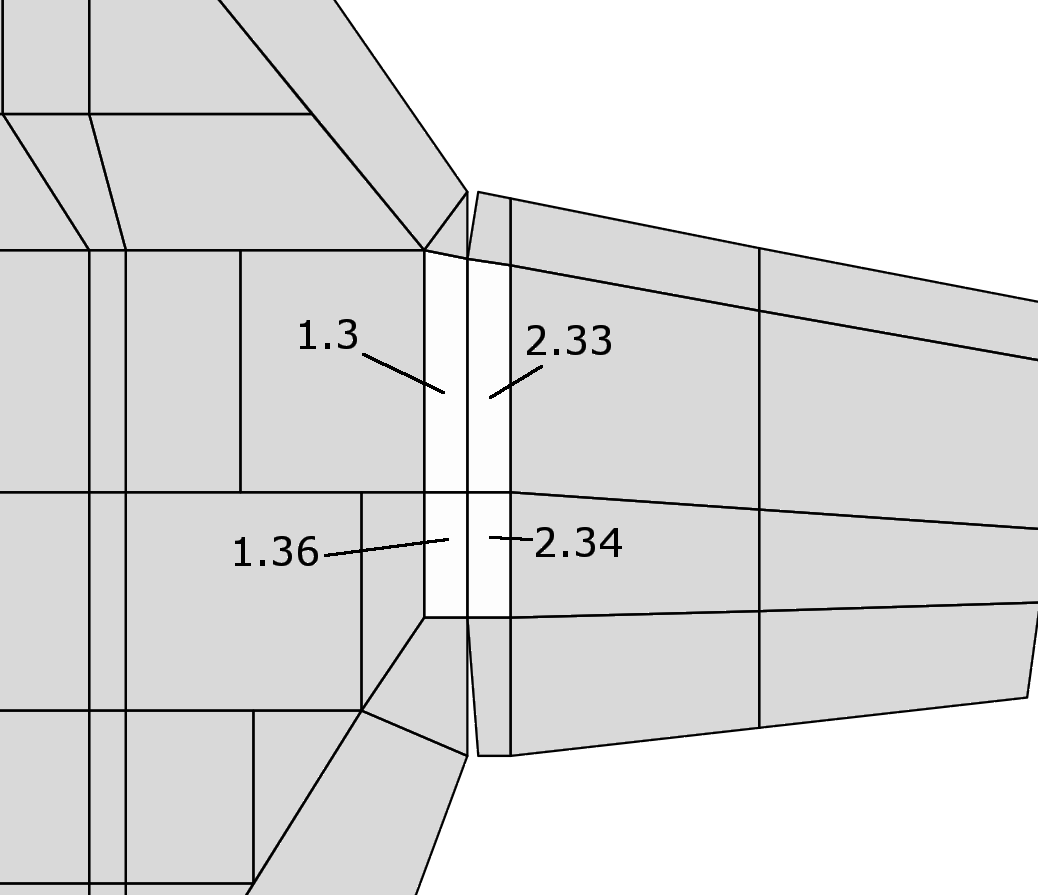
\includegraphics[width=0.5\textwidth]{RootOfWingWithSelectedPartsBW}
\caption{Схематичное изображение вида сверху в месте стыка правого крыла и фюзеляжа}
\label{fig:WingRootPlain}
\end{figure}




Исходя из полученных данных, была получена зависимость величины средних напряжений в панелях и стенках этих отсеков от выбора размера конечного элемента (Рис.\ref{fig:stressToDiscreteness})

\begin{figure}[ht]
\centering
%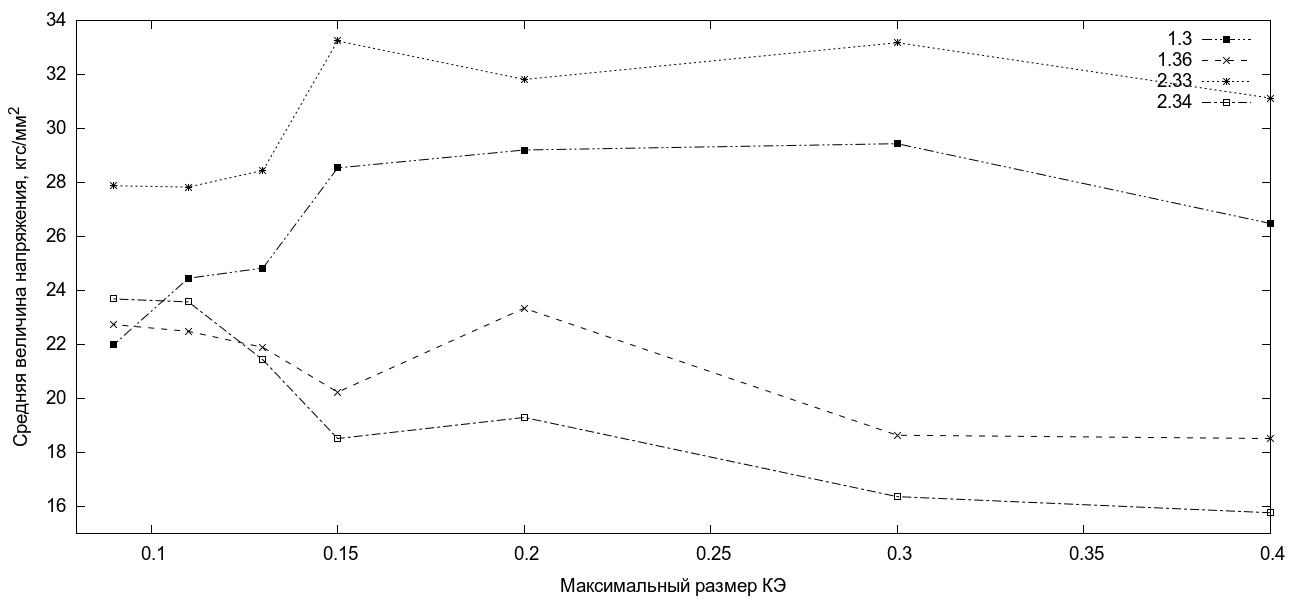
\includegraphics[width=0.8\textwidth]{StressToDiscretenessPlot}
% GNUPLOT: LaTeX picture with Postscript
\begingroup
  \makeatletter
  \providecommand\color[2][]{%
    \GenericError{(gnuplot) \space\space\space\@spaces}{%
      Package color not loaded in conjunction with
      terminal option `colourtext'%
    }{See the gnuplot documentation for explanation.%
    }{Either use 'blacktext' in gnuplot or load the package
      color.sty in LaTeX.}%
    \renewcommand\color[2][]{}%
  }%
  \providecommand\includegraphics[2][]{%
    \GenericError{(gnuplot) \space\space\space\@spaces}{%
      Package graphicx or graphics not loaded%
    }{See the gnuplot documentation for explanation.%
    }{The gnuplot epslatex terminal needs graphicx.sty or graphics.sty.}%
    \renewcommand\includegraphics[2][]{}%
  }%
  \providecommand\rotatebox[2]{#2}%
  \@ifundefined{ifGPcolor}{%
    \newif\ifGPcolor
    \GPcolorfalse
  }{}%
  \@ifundefined{ifGPblacktext}{%
    \newif\ifGPblacktext
    \GPblacktexttrue
  }{}%
  % define a \g@addto@macro without @ in the name:
  \let\gplgaddtomacro\g@addto@macro
  % define empty templates for all commands taking text:
  \gdef\gplbacktext{}%
  \gdef\gplfronttext{}%
  \makeatother
  \ifGPblacktext
    % no textcolor at all
    \def\colorrgb#1{}%
    \def\colorgray#1{}%
  \else
    % gray or color?
    \ifGPcolor
      \def\colorrgb#1{\color[rgb]{#1}}%
      \def\colorgray#1{\color[gray]{#1}}%
      \expandafter\def\csname LTw\endcsname{\color{white}}%
      \expandafter\def\csname LTb\endcsname{\color{black}}%
      \expandafter\def\csname LTa\endcsname{\color{black}}%
      \expandafter\def\csname LT0\endcsname{\color[rgb]{1,0,0}}%
      \expandafter\def\csname LT1\endcsname{\color[rgb]{0,1,0}}%
      \expandafter\def\csname LT2\endcsname{\color[rgb]{0,0,1}}%
      \expandafter\def\csname LT3\endcsname{\color[rgb]{1,0,1}}%
      \expandafter\def\csname LT4\endcsname{\color[rgb]{0,1,1}}%
      \expandafter\def\csname LT5\endcsname{\color[rgb]{1,1,0}}%
      \expandafter\def\csname LT6\endcsname{\color[rgb]{0,0,0}}%
      \expandafter\def\csname LT7\endcsname{\color[rgb]{1,0.3,0}}%
      \expandafter\def\csname LT8\endcsname{\color[rgb]{0.5,0.5,0.5}}%
    \else
      % gray
      \def\colorrgb#1{\color{black}}%
      \def\colorgray#1{\color[gray]{#1}}%
      \expandafter\def\csname LTw\endcsname{\color{white}}%
      \expandafter\def\csname LTb\endcsname{\color{black}}%
      \expandafter\def\csname LTa\endcsname{\color{black}}%
      \expandafter\def\csname LT0\endcsname{\color{black}}%
      \expandafter\def\csname LT1\endcsname{\color{black}}%
      \expandafter\def\csname LT2\endcsname{\color{black}}%
      \expandafter\def\csname LT3\endcsname{\color{black}}%
      \expandafter\def\csname LT4\endcsname{\color{black}}%
      \expandafter\def\csname LT5\endcsname{\color{black}}%
      \expandafter\def\csname LT6\endcsname{\color{black}}%
      \expandafter\def\csname LT7\endcsname{\color{black}}%
      \expandafter\def\csname LT8\endcsname{\color{black}}%
    \fi
  \fi
  \setlength{\unitlength}{0.0500bp}%
  \begin{picture}(8502.00,4534.00)%
    \gplgaddtomacro\gplbacktext{%
      \csname LTb\endcsname%
      \put(814,892){\makebox(0,0)[r]{\strut{} 16}}%
      \put(814,1267){\makebox(0,0)[r]{\strut{} 18}}%
      \put(814,1642){\makebox(0,0)[r]{\strut{} 20}}%
      \put(814,2017){\makebox(0,0)[r]{\strut{} 22}}%
      \put(814,2393){\makebox(0,0)[r]{\strut{} 24}}%
      \put(814,2768){\makebox(0,0)[r]{\strut{} 26}}%
      \put(814,3143){\makebox(0,0)[r]{\strut{} 28}}%
      \put(814,3518){\makebox(0,0)[r]{\strut{} 30}}%
      \put(814,3894){\makebox(0,0)[r]{\strut{} 32}}%
      \put(814,4269){\makebox(0,0)[r]{\strut{} 34}}%
      \put(1393,484){\makebox(0,0){\strut{} 0.1}}%
      \put(2512,484){\makebox(0,0){\strut{} 0.15}}%
      \put(3631,484){\makebox(0,0){\strut{} 0.2}}%
      \put(4749,484){\makebox(0,0){\strut{} 0.25}}%
      \put(5868,484){\makebox(0,0){\strut{} 0.3}}%
      \put(6986,484){\makebox(0,0){\strut{} 0.35}}%
      \put(8105,484){\makebox(0,0){\strut{} 0.4}}%
      \put(176,2486){\rotatebox{-270}{\makebox(0,0){\strut{}Средняя величина напряжения, $\text{кгс}/\text{мм}^2$}}}%
      \put(4525,154){\makebox(0,0){\strut{}Максимальный размер КЭ}}%
    }%
    \gplgaddtomacro\gplfronttext{%
      \csname LTb\endcsname%
      \put(7118,4096){\makebox(0,0)[r]{\strut{}$1.3$}}%
      \csname LTb\endcsname%
      \put(7118,3876){\makebox(0,0)[r]{\strut{}$1.36$}}%
      \csname LTb\endcsname%
      \put(7118,3656){\makebox(0,0)[r]{\strut{}$2.33$}}%
      \csname LTb\endcsname%
      \put(7118,3436){\makebox(0,0)[r]{\strut{}$2.34$}}%
    }%
    \gplbacktext
    \put(0,0){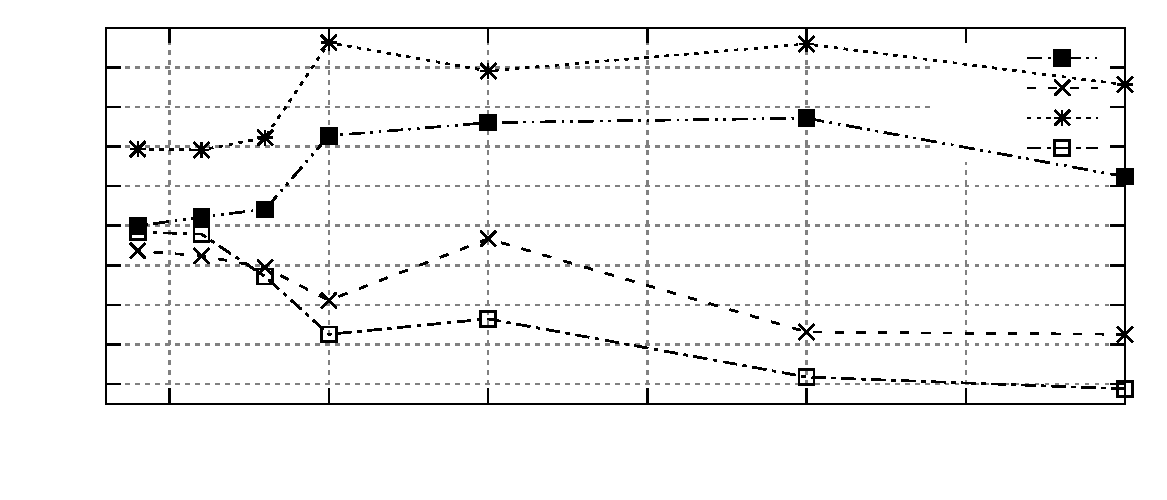
\includegraphics{StressToDiscreteness}}%
    \gplfronttext
  \end{picture}%
\endgroup

\caption{Зависимость средних напряжений в отсеках от величины КЭ}
\label{fig:stressToDiscreteness}
\end{figure}

На основании полученных данных и исходя из трудоемкости процесса расчета модели была определена оптимальная величина конечного элемента для дальнейшей работы над моделью, принятая равной $0,11\text{м}$. 
%Ниже приведены картины НДС в месте стыка крыла с фюзеляжем при различных размерах конечного элемента. 
\subsection{Проблемы проектирования}

В предложенной конструкторами схеме были выявлены некоторые проблемные места, в которых требовался дополнительный анализ. 

 \paragraph{Крепление хвостовой части к кессону центроплана} 
\label{sec:pants}
\begin{figure}[H]
\centering
\def\svgwidth{\textwidth}
\input{figures/IsoviewOfPants.pdf_tex}
%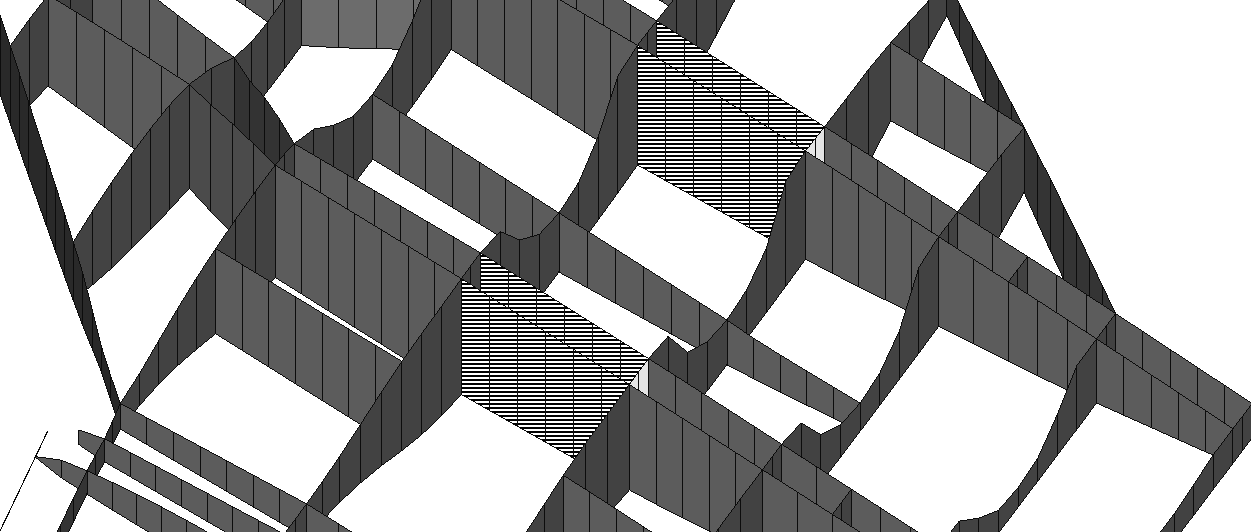
\includegraphics[width=0.6\textwidth]{IsoviewOfPantsBW}
\caption{Вид каркаса фюзеляжа}
\label{fig:IsoviewOfPants}
\end{figure}


Для частичной валидации решения, полученного в результате определния рациональных параметров (см. предыдущий раздел), была решена модельная задача по оценке устойчивости центральных стенок, обеспечивающих крепление хвостовой части гипотетического БПЛА к его центроплану (данные стенки обозначены на Рис.~\ref{fig:IsoviewOfPants} серой заливкой, светло-серой заливкой обозначены зоны основных узлов крепления двигателя). Эти стенки были нагружены перерезывающими усилиями, и необходима была проверка их по условиям устойчивости, которая не проводилась для этих элементов конструкции в процессе определения рациональных параметров. НДС стенок был оценен на основе аналитических формул. Схема нагружения модельных стенок показана на Рис.\ref{fig:IsoviewOfPantsModel}.

\begin{figure}[H]
\centering
%\def\svgwidth{0.9\textwidth}
\input{figures/IsoviewOfPantsModel.pdf_tex}
\caption{Схема нагружения модельных стенок}
\label{fig:IsoviewOfPantsModel}
\end{figure}

%
%\begin{figure}[H]
%\centering
%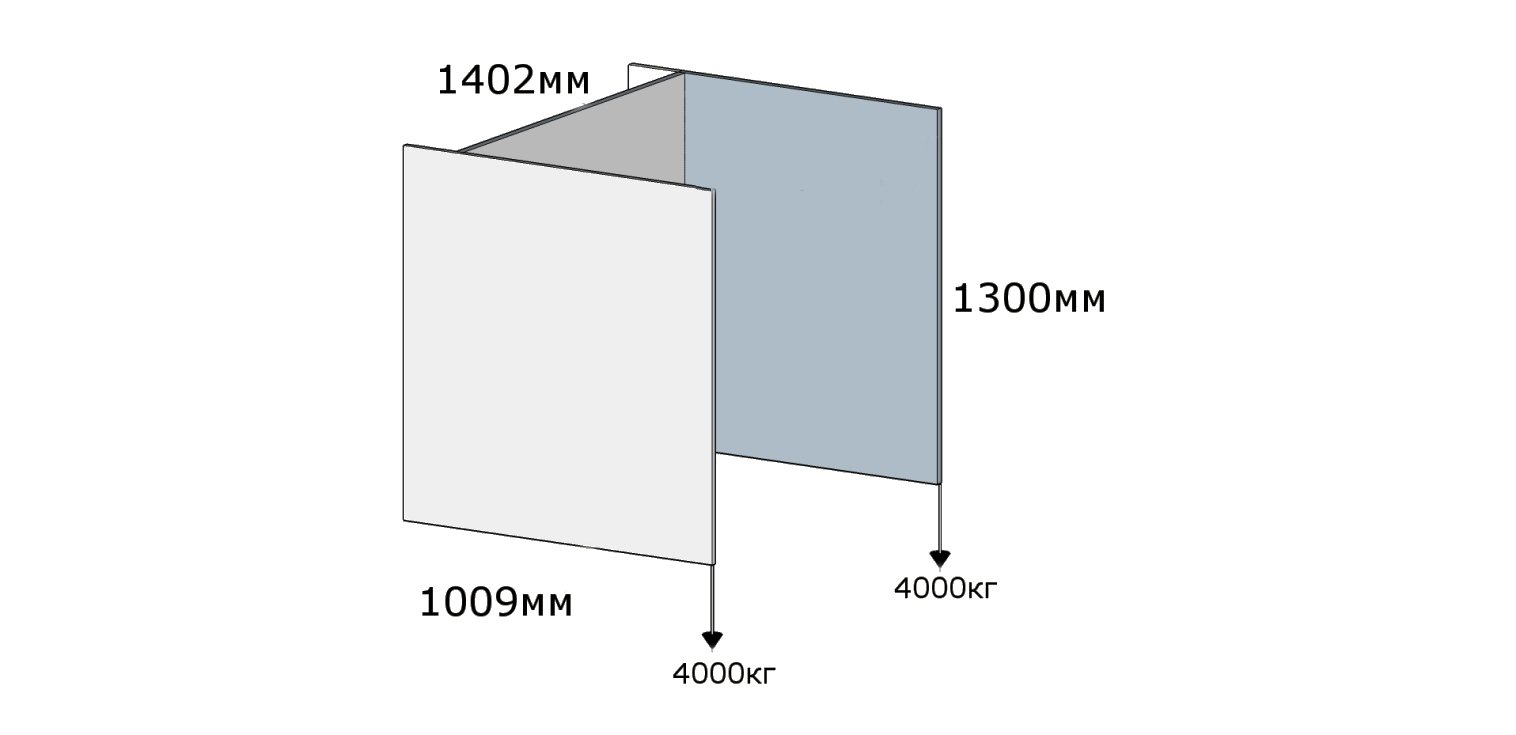
\includegraphics[width=0.8\textwidth]{IsoviewOfPantsModel}
%\caption{Схема нагружения модельных стенок}
%\label{IsoviewOfPantsModel}
%\end{figure}


Уровень нагружения был оценен по величинам касательных напряжений. Касательные напряжения в пластине при чистом сдвиге равны

\begin{equation}
\tau=\frac{3}{2}\cdot\frac{Q}{bh}
\end{equation}
Критические по устойчивости касательные напряжения в пластине при чистом сдвиге равны \cite{Volmir}:

\begin{equation}
\tau_\text{кр}=\frac{K}{12}\frac{\pi^2D}{b^2h} = \frac{K}{12}\frac{\pi^2E}{(1-\mu^2)}\left(\frac{h}{b}\right)^2,\, K=5.34 + 4\frac{a}{b},
\end{equation}
где $a$ - размер пластины вдоль направления действия силы, $b$ - размер пластины поперек направления действия силы, $h$ - толщина пластины, $D$ - изгибная жесткость пластины, $E$ - модуль Юнга, $\mu$ - модуль Пуассона материала пластины, $Q$ - приложенная сила.
Допускаемые толщины найдем из условия:

\begin{equation}
\tau_\text{кр} \geq \tau  
\end{equation}

\begin{equation}
h \geq \sqrt[3]{\frac{3\cdot12}{2}\frac{Qb\cdot(1-\mu^2)}{k\pi^2E}}
\end{equation}

Подставляя значения, получим:

\begin{equation}
Q=\frac{8000}{n}\text{кгс},\,a=1300\text{мм},\,b=1009\text{мм},\,\mu=0.3,\,E=7000\frac{\text{кгс}}{\text{мм}^2}
\end{equation}

\begin{equation}
h \geq \sqrt[3]{\frac{18\cdot8000\cdot1000\cdot(1-\mu^2)}{k\pi^2En}} = \frac{5.67}{\sqrt[3]{n}} 
\end{equation}

Таким образом, для случаев $n = 2$ и $n = 4$  были получены минимальные допустимые толщины, 
равные:

\begin{equation}
h\geq4.50\text{мм},\,n=2
\end{equation}
\begin{equation}
h\geq2.83\text{мм},\,n=4
\label{eq:pants_n4}
\end{equation}

Рациональные значения толщин исследуемых обшивок, полученные в данном проектировочном исследовании, оказались меньше ($h = 1\text{мм}$), чем приведенные в \ref{eq:pants_n4}. Таким образом, выполнение условий по устойчивости этих стенок привело к увеличению их толщин. Более рациональным способом увеличения сдвиговой жесткости этих стенок является использование ферменных подкрепляющих элементов.
\subsubsection{Фюзеляжная часть центроплана}

Другим проблемным местом была фюзеляжная часть центроплана. Из-за требований компоновки, а именно интеграции двигателя, центроплан необходимо делать изогнутым (Рис.\ref{fig:centroplan}). Это вносит дополнительные трудности в виде увеличения веса по сравнению с прямым центропланом. Исследованию фюзеляжной части центроплана (выделена серым на Рис.\ref{fig:centroplan}) посвящена глава \ref{chap:SolvingModel}.

\begin{figure}[ht]
\centering
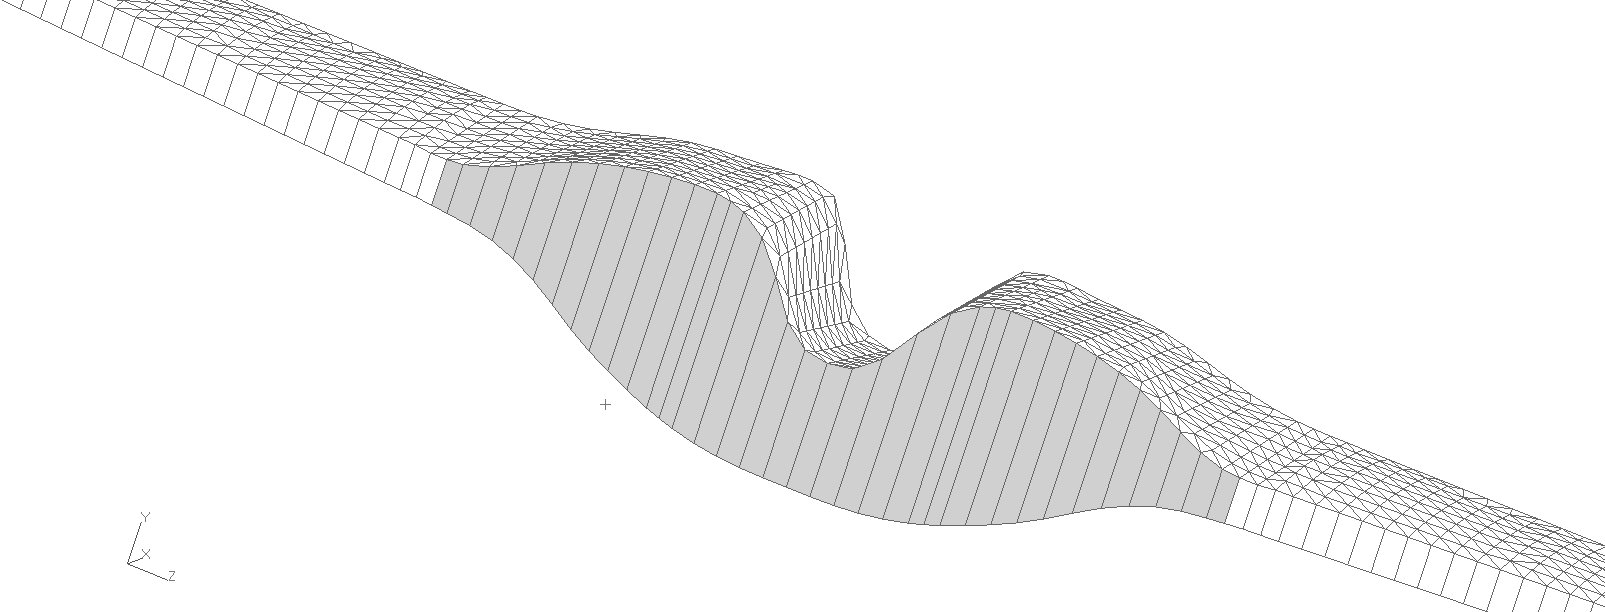
\includegraphics[width=0.6\textwidth]{centroplan}
\caption{Изогнутый центроплан с выделением исследуемой части}
\label{fig:centroplan}
\end{figure}


%\chapter{Решение модельной задачи}
\label{chap:SolvingModel}

\section{Создание параметрической модели центроплана}
\label{sec:creationOfModel}

В рамках решения данной модельной задачи на базе общей МКЭ-модели гипотетической конструкции БПЛА (Рис.\ref{fig:fullMKE}) была создана упрощенная параметрическая модель центроплана, представляющая из себя подробную МКЭ-модель центроплана. В упрощенной модели кессон фюзеляжной части центроплана (Рис.\ref{fig:centroplanMKE}) заменен коробом переменного прямоугольного сечения с поперечными стенками. На короб передаются усилия аналогичные усилиям, приходящим с крыла для конструкции гипотетического БПЛА, путем приложения аэродинамических нагрузок на упрощенную модель крыла -- короб постоянного прямоугольного сечения (Рис.\ref{fig:simplifiedCentroplanMKE}). Материал - дюраль, панели и стенки центропланов имеют постоянную по площади толщину, без вырезов. Носовая и хвостовая части самолета опущены для простоты расчета.  


\begin{figure}[ht]
\centering 
\includegraphics[width=0.9\textwidth]{BPLAfullModel}
\caption{МКЭ-модель гипотетической конструкции БПЛА}
\label{fig:fullMKE}
\end{figure}

\begin{figure}[ht]
\centering 
\includegraphics[width=0.9\textwidth]{centroplan}
\caption{МКЭ-модель центроплана гипотетической конструкции БПЛА}
\label{fig:centroplanMKE}
\end{figure}

\begin{figure}[ht]
\centering
\includegraphics[width=0.9\textwidth]{simplifiedCentroplan}
\caption{Упрощенная МКЭ-модель центроплана}
\label{fig:simplifiedCentroplanMKE}
\end{figure}

Использование в МКЭ-расчете такой упрощенной модели позволяет значительно ускорить процесс прочностного параметрического анализа при тех же вычислительных мощностях. Так, в упрощенной модели используется $\approx10000$ конечных элементов, в то время как в МКЭ-модели полного БПЛА используется $\approx270000$ конечных элементов.

Как было сказано выше, рассматриваемая модель определяется двумя базовыми параметрами: координатой нижней точки сечения относительно базовой горизонтали БПЛА $y_\text{отн}$ и строительной высотой сечения в плоскости симметрии самолета $h_\text{стр}$. В качестве кривых, описывающих нижнюю и верхнюю поверхность кессона выбраны кубические сплайны, построенные через найденные исходя из выбранных параметров точки. Производные сплайнов в точках стыка фюзеляжа с крылом ($z=2.45\text{м}$) и в плоскости симметрии самолета ($z=0\text{м}$) приняты равными нулю. Пример модельного сечения центроплана в плоскости YZ со значениями параметров $h_\text{стр}=0.4\text{м}$, $y_\text{отн} = -1.4\text{м}$ приведен на Рис.\ref{fig:KessSectionExample}.

\begin{figure}[ht]
\centering
\def\svgwidth{\textwidth}
%\includegraphics[width=1\textwidth]{KessSectionExample}
\input{figures/KessSectionExample.pdf_tex}
\caption{Пример формируемого параметрически поперечного сечения центроплана}
\label{fig:KessSectionExample}
\end{figure}


\subsection{Внесенные изменения}

В ходе работы, для повышения степени автоматизации процесса был создан новый интерфейс  для первого уровня комплекса. 

\begin{figure}[h]
\centering
\includegraphics[width=0.8\textwidth]{ConverNewInterfaceOverview}
\caption{Новый интерфейс программного комплекса ``Conver''}
\label{fig:ConverNewInterfaceOverview}
\end{figure}


В новом интерфейсе были реализованы следующие изменения:

\begin{itemize}
	\item Полностью переработана система визуализации
	\begin{itemize}
		\item Добавлены инструменты масштаба и перемещения
		\item Добавлена двусторонняя связь между схемой и областями ввода данных
		\item Добавлена возможность отображения каждого этажа в 		схеме по отдельности
		\item Добавлено отображение ошибок во введенных данных
	\end{itemize}
	\item Переработана система ввода параметров отсеков
	\begin{itemize}
		\item Добавлены визуальные подсказки, предупреждающие ошибки в данных
		\item Добавлена возможность ввода параметров сразу для нескольких отсеков
	\end{itemize}
	\item Добавлена возможность ввода нагрузок непосредственно через задание сил, действующих на отсек
	\item Добавлена возможность просмотра данных, получаемых из других уровней комплекса:
	\begin{itemize}
		\item Оценочный расчет веса конструкции или выбранных отсеков
		\item Расчет объема выбранных отсеков
		\item Просмотр площадей стенок отсеков
	\end{itemize}
\end{itemize}

Рассмотрим, как изменилась работа с типовыми операциями, с которыми приходится сталкиваться пользователю. 


\subsection{Сравнение работы с типовыми операциями в старой и новой версии интерфейса}

\subsubsection{Изменение толщин в отсеке}

Задача: изменить толщину отсека в центроплане. 

\paragraph{Прежний подход:} 

\begin{itemize}
\item Найти номер отсека по схеме (Рис.\ref{fig:ConverListxzOld}) ($\sim1-3~\text{мин.}$)
\item Найти соответствующую ячейку в таблице толщин. ($\sim15~\text{сек.}$)
\item Изменить значение в ячейке. ($\sim5~\text{сек.}$)
\end{itemize}

Итого: $\sim3~\text{мин.}$

\begin{figure}[ht]
\centering
\includegraphics[width=0.8\textwidth]{ConverListxzOld}
\caption{Окно отображения отсеков в предыдущей версии интерфейса}
\label{fig:ConverListxzOld}
\end{figure}

\paragraph{Новый подход:}

\begin{itemize}
\item Кликнуть на нужный отсек на схеме (Рис.\ref{fig:ConverListxzOld}) ($\sim5~\text{сек.}$)
\item Изменить значение в ячейке толщины нужной стенки($\sim5~\text{сек.}$)
\end{itemize}

Итого: $\sim10~\text{сек.}$

\begin{figure}[ht]
\centering
\includegraphics[width=0.8\textwidth]{ConverNewChangingThicks}
\caption{Окно отображения отсеков в новой версии интерфейса}
\label{ConverNewChangingThicks}
\end{figure}

\subsubsection{Нагружение отсека заданной силой}

Задача: по визуальному нахождению стенки нагрузить её заданной силой.

\paragraph{Прежний подход:}

\begin{itemize}
\item Найти по схеме (Рис.\ref{fig:ConverListxzOld}) отсеки, в которых может быть определена нужная стенка ($\sim5~\text{мин.}$)
\item Найти в таблице толщин, какой из выбранных отсеков имеет толщину этой стенки отличную от нуля($\sim3~\text{мин.}$)
\item Из 4 уровня программы найти площадь этой стенки($\sim3~\text{мин.}$)
\item По площади стенки найти давление, которое необходимо на неё приложить($\sim1~\text{мин.}$)
\item В таблице давлений найти нужную ячейку и ввести в неё полученную величину($\sim5~\text{мин.}$)
\end{itemize}

Итого: $\sim17~\text{мин.}$

\paragraph{Новый подход:}

\begin{itemize}
\item Кликнуть на один из отсеков, которому принадлежит эта стенка($\sim10~\text{сек.}$)
\item Если ячейка давления на нужную стенку выделена красным, выбрать другой отсек, в котором эта ячейка не выделена красным, то есть в которой эта стенка имеет ненулевую толщину($\sim1~\text{мин.}$)
\item Нажать кнопку ``Add load''  ($\sim10~\text{сек.}$)
\item В открывшемся окне (Рис.\ref{fig:ConverAddLoad}) ввести величину прикладываемой силы и выбрать стенки отсека, на которые должна быть распределена данная нагрузка. ($\sim30~\text{сек.}$) 
\item Нажать ``Add load'' ($\sim10~\text{сек.}$)

\end{itemize}

Итого: $\sim2~\text{мин.}$

\begin{figure}[ht]
\centering
\includegraphics[width=0.5\textwidth]{ConverNewInterfaceAddLoad}
\caption{Окно добавления нагрузок в новой версии интерфейса}
\label{fig:ConverAddLoad}
\end{figure}
\section{Расчет параметрической модели}
\label{sec:calculationOfModel}
Для проведения параметрического расчета были выбраны 42 пары значений параметров. Для каждой пары значений была проведена оптимизация толщин панелей модели с целью удовлетворения требованиям прочности конструкции. Оптимизация была проведена путем многократных нахождения запаса прочности для каждой панели (стенки отсека) с последующим делением толщины панели на полученное значение (так называемый алгоритм $\sigma/\sigma$). Итоговые результаты вычислений приведены в таблицах \ref{tab:KessTableNormedComparison}, \ref{tab:KessOptimBigTableNormed} и на Рис.\ref{fig:Optimization3dplot} (серым цветом на изображениях сечений показано оригинальное сечение кессона в гипотетической модели БПЛА-ЦАГИ, зеленым - сечение в параметрической модели)  

%%%%%%%%%%%%%%%%%%%%%%%%%%%%%%%%%%


\tabulinesep = 1mm
\definecolor{lightgray}{gray}{0.9}
\begin{table}[ht]
    \fontsize{11pt}{12pt}\selectfont
\captionsetup{justification=centering}
\caption{Зависимость веса кессона от параметров центроплана относительно варианта с прямым кессоном}
%\rowcolors{2}{}{lightgray}
\begin{tabu}to \linewidth{|>{\columncolor{lightgray}}c|*8{X[m c]|}}
\hline
%\taburowcolors {lightgray .. white}
\rowcolor{lightgray}
$h_\text{стр} \setminus y_\text{отн}$		&	0.000	&	-0.800	&	-1.000	&	-1.100	&	-1.200	&	-1.300	&	-1.400  \\ \hline 
0.249	&	1.000	&	1.278	&	1.330	&	1.370	&	1.397	&	1.449	&	1.548	\\ \hline
0.403	&	0.811	&	0.937	&	0.971	&	0.993	&	1.027	&	1.053	&	1.078	\\ \hline
0.481	&	0.764	&	0.824	&	0.862	&	0.873	&	0.895	&	0.933	&	0.953	\\ \hline
0.558	&	0.726	&	0.755	&	0.792	&	0.790	&	0.824	&	0.833	&	0.857	\\ \hline
0.635	&	0.684	&	0.723	&	0.731	&	0.768	&	0.756	&	0.784	&	0.797	\\ \hline
0.712	&	0.657	&	0.697	&	0.721	&	0.717	&	0.735	&	0.746	&	0.757	\\ \hline
\end{tabu}

\label{tab:KessTableNormedComparison}
\end{table}

%\tabulinesep = 1mm
%\definecolor{lightgray}{gray}{0.9}
%\begin{table}[H]
%
%
%    \fontsize{12pt}{14pt}\selectfont
%\captionsetup{justification=centering}
%\caption{Зависимость площади панелей центроплана и веса кессона от параметров центроплана (данные надо пересчитывать)}
%%\rowcolors{2}{}{lightgray}
%\begin{tabu}to \linewidth{|c|*4{X[m c]|}*4{X[m c]|}}
%\hline
%\multirow{2}{*}[-1.1ex]{N} & \multicolumn{4}{c|}{Вес кессона~[кг]} & \multicolumn{4}{c|}{Площадь панелей центроплана~[$\text{м}^2$]} \\ \cline{2-9}
%& Верхние панели & Нижние панели & Боковые стенки & $\Sigma$ & Верхние панели & Нижние панели & Боковые стенки & $\Sigma$ \\
%\hline
%\taburowcolors {lightgray .. white}
%1 & 297.182 & 294.551 & 12.561 & 604.294 & 2.730 & 2.730 & 4.000 & 9.520\\ \hline
2 & 225.261 & 237.378 & 27.672 & 490.313 & 2.730 & 2.740 & 5.210 & 10.720\\ \hline
3 & 190.080 & 222.327 & 49.159 & 461.564 & 2.730 & 2.760 & 5.820 & 11.340\\ \hline
4 & 161.544 & 211.467 & 65.963 & 438.972 & 2.730 & 2.760 & 6.450 & 11.950\\ \hline
5 & 146.581 & 199.989 & 66.844 & 413.415 & 2.730 & 2.780 & 7.090 & 12.590\\ \hline
6 & 134.746 & 191.293 & 70.912 & 396.952 & 2.730 & 2.800 & 7.640 & 13.200\\ \hline
7 & 350.816 & 374.021 & 47.679 & 772.515 & 2.910 & 2.910 & 4.000 & 9.850\\ \hline
8 & 253.752 & 259.311 & 53.180 & 566.245 & 2.910 & 2.850 & 5.210 & 10.990\\ \hline
9 & 213.881 & 226.655 & 57.618 & 498.154 & 2.910 & 2.830 & 5.840 & 11.570\\ \hline
10 & 188.442 & 205.603 & 62.047 & 456.092 & 2.910 & 2.810 & 6.450 & 12.150\\ \hline
11 & 174.466 & 196.192 & 66.506 & 437.164 & 2.910 & 2.780 & 7.090 & 12.770\\ \hline
12 & 154.328 & 195.919 & 70.963 & 421.210 & 2.910 & 2.770 & 7.680 & 13.350\\ \hline
13 & 363.681 & 391.414 & 48.862 & 803.953 & 3.010 & 3.000 & 4.000 & 10.000\\ \hline
14 & 258.118 & 275.555 & 53.209 & 586.883 & 3.010 & 2.930 & 5.230 & 11.160\\ \hline
15 & 225.322 & 238.220 & 57.604 & 521.145 & 3.010 & 2.890 & 5.820 & 11.720\\ \hline
16 & 201.612 & 214.755 & 62.046 & 478.413 & 3.010 & 2.860 & 6.440 & 12.310\\ \hline
17 & 171.877 & 203.370 & 66.418 & 441.665 & 3.010 & 2.840 & 7.050 & 12.900\\ \hline
18 & 163.553 & 201.207 & 70.912 & 435.673 & 3.010 & 2.820 & 7.660 & 13.480\\ \hline
19 & 380.079 & 398.521 & 49.032 & 827.631 & 3.050 & 3.050 & 4.000 & 10.110\\ \hline
20 & 267.143 & 279.590 & 53.134 & 599.866 & 3.050 & 2.980 & 5.210 & 11.240\\ \hline
21 & 231.158 & 238.954 & 57.667 & 527.779 & 3.050 & 2.930 & 5.820 & 11.820\\ \hline
22 & 197.327 & 218.001 & 62.040 & 477.368 & 3.050 & 2.910 & 6.410 & 12.390\\ \hline
23 & 191.553 & 205.935 & 66.481 & 463.971 & 3.050 & 2.870 & 7.070 & 12.980\\ \hline
24 & 158.352 & 203.948 & 70.897 & 433.199 & 3.050 & 2.850 & 7.660 & 13.560\\ \hline
25 & 383.525 & 410.374 & 50.351 & 844.249 & 3.110 & 3.110 & 4.000 & 10.210\\ \hline
26 & 279.228 & 288.331 & 53.186 & 620.745 & 3.110 & 3.030 & 5.210 & 11.350\\ \hline
27 & 233.614 & 249.500 & 57.583 & 540.696 & 3.110 & 2.990 & 5.820 & 11.910\\ \hline
28 & 213.922 & 221.683 & 62.125 & 497.728 & 3.110 & 2.950 & 6.450 & 12.500\\ \hline
29 & 180.457 & 210.067 & 66.523 & 457.046 & 3.110 & 2.920 & 7.070 & 13.070\\ \hline
30 & 167.492 & 205.426 & 71.001 & 443.918 & 3.110 & 2.880 & 7.640 & 13.660\\ \hline
31 & 401.418 & 424.040 & 50.413 & 875.868 & 3.160 & 3.160 & 4.000 & 10.330\\ \hline
32 & 285.115 & 297.451 & 53.649 & 636.214 & 3.160 & 3.070 & 5.230 & 11.470\\ \hline
33 & 251.131 & 255.015 & 57.656 & 563.801 & 3.160 & 3.040 & 5.860 & 12.030\\ \hline
34 & 212.049 & 229.543 & 62.067 & 503.658 & 3.160 & 3.000 & 6.450 & 12.610\\ \hline
35 & 191.030 & 215.968 & 66.550 & 473.548 & 3.160 & 2.970 & 7.070 & 13.170\\ \hline
36 & 170.765 & 209.184 & 70.962 & 450.912 & 3.160 & 2.920 & 7.660 & 13.740\\ \hline
37 & 431.880 & 451.562 & 51.974 & 935.418 & 3.230 & 3.230 & 4.000 & 10.440\\ \hline
38 & 291.199 & 306.178 & 54.263 & 651.640 & 3.230 & 3.130 & 5.210 & 11.560\\ \hline
39 & 253.054 & 265.073 & 57.593 & 575.719 & 3.230 & 3.090 & 5.820 & 12.140\\ \hline
40 & 222.782 & 233.403 & 61.948 & 518.132 & 3.230 & 3.050 & 6.400 & 12.700\\ \hline
41 & 197.192 & 218.301 & 66.423 & 481.917 & 3.230 & 3.020 & 7.030 & 13.270\\ \hline
42 & 175.591 & 210.828 & 70.877 & 457.295 & 3.230 & 2.970 & 7.660 & 13.840\\ \hline
%\end{tabu}
%
%\label{tab:KessOptimBigTable}
%\end{table}

%%%%%%%%%%%%%%%%%%%%%%%%%%%%%%%%%

\tabulinesep = 1mm
\definecolor{lightgray}{gray}{0.9}
\begin{table}[ht]
    \fontsize{11pt}{12pt}\selectfont
\captionsetup{justification=centering}
\caption{Зависимость площади панелей центроплана и веса кессона от параметров центроплана относительно варианта с прямым кессоном}
%\rowcolors{2}{}{lightgray}
\begin{tabu}to \linewidth{|c|c|*4{X[m c]|}*4{X[m c]|}}
\hline
\multirow{2}{*}[-1.1ex]{$y_\text{отн}$} & \multirow{2}{*}[-1.1ex]{$h_\text{стр}$} & \multicolumn{4}{c|}{Вес кессона} & \multicolumn{4}{c|}{Площадь панелей центроплана} \\ \cline{3-9}
& & Верхние панели & Нижние панели & Боковые стенки & $\Sigma$ & Верхние панели & Нижние панели & Боковые стенки & $\Sigma$ \\
\hline
\taburowcolors {lightgray .. white}
1 & 0.492 & 0.487 & 0.021 & 1.000 & 0.287 & 0.287 & 0.420 & 1.000\\ \hline
2 & 0.373 & 0.393 & 0.046 & 0.811 & 0.287 & 0.288 & 0.547 & 1.126\\ \hline
3 & 0.315 & 0.368 & 0.081 & 0.764 & 0.287 & 0.290 & 0.611 & 1.191\\ \hline
4 & 0.267 & 0.350 & 0.109 & 0.726 & 0.287 & 0.290 & 0.678 & 1.255\\ \hline
5 & 0.243 & 0.331 & 0.111 & 0.684 & 0.287 & 0.292 & 0.745 & 1.322\\ \hline
6 & 0.223 & 0.317 & 0.117 & 0.657 & 0.287 & 0.294 & 0.803 & 1.387\\ \hline
7 & 0.581 & 0.619 & 0.079 & 1.278 & 0.306 & 0.306 & 0.420 & 1.035\\ \hline
8 & 0.420 & 0.429 & 0.088 & 0.937 & 0.306 & 0.299 & 0.547 & 1.154\\ \hline
9 & 0.354 & 0.375 & 0.095 & 0.824 & 0.306 & 0.297 & 0.613 & 1.215\\ \hline
10 & 0.312 & 0.340 & 0.103 & 0.755 & 0.306 & 0.295 & 0.678 & 1.276\\ \hline
11 & 0.289 & 0.325 & 0.110 & 0.723 & 0.306 & 0.292 & 0.745 & 1.341\\ \hline
12 & 0.255 & 0.324 & 0.117 & 0.697 & 0.306 & 0.291 & 0.807 & 1.402\\ \hline
13 & 0.602 & 0.648 & 0.081 & 1.330 & 0.316 & 0.315 & 0.420 & 1.050\\ \hline
14 & 0.427 & 0.456 & 0.088 & 0.971 & 0.316 & 0.308 & 0.549 & 1.172\\ \hline
15 & 0.373 & 0.394 & 0.095 & 0.862 & 0.316 & 0.304 & 0.611 & 1.231\\ \hline
16 & 0.334 & 0.355 & 0.103 & 0.792 & 0.316 & 0.300 & 0.676 & 1.293\\ \hline
17 & 0.284 & 0.337 & 0.110 & 0.731 & 0.316 & 0.298 & 0.741 & 1.355\\ \hline
18 & 0.271 & 0.333 & 0.117 & 0.721 & 0.316 & 0.296 & 0.805 & 1.416\\ \hline
19 & 0.629 & 0.659 & 0.081 & 1.370 & 0.320 & 0.320 & 0.420 & 1.062\\ \hline
20 & 0.442 & 0.463 & 0.088 & 0.993 & 0.320 & 0.313 & 0.547 & 1.181\\ \hline
21 & 0.383 & 0.395 & 0.095 & 0.873 & 0.320 & 0.308 & 0.611 & 1.242\\ \hline
22 & 0.327 & 0.361 & 0.103 & 0.790 & 0.320 & 0.306 & 0.673 & 1.301\\ \hline
23 & 0.317 & 0.341 & 0.110 & 0.768 & 0.320 & 0.301 & 0.743 & 1.363\\ \hline
24 & 0.262 & 0.337 & 0.117 & 0.717 & 0.320 & 0.299 & 0.805 & 1.424\\ \hline
25 & 0.635 & 0.679 & 0.083 & 1.397 & 0.327 & 0.327 & 0.420 & 1.072\\ \hline
26 & 0.462 & 0.477 & 0.088 & 1.027 & 0.327 & 0.318 & 0.547 & 1.192\\ \hline
27 & 0.387 & 0.413 & 0.095 & 0.895 & 0.327 & 0.314 & 0.611 & 1.251\\ \hline
28 & 0.354 & 0.367 & 0.103 & 0.824 & 0.327 & 0.310 & 0.678 & 1.313\\ \hline
29 & 0.299 & 0.348 & 0.110 & 0.756 & 0.327 & 0.307 & 0.743 & 1.373\\ \hline
30 & 0.277 & 0.340 & 0.117 & 0.735 & 0.327 & 0.303 & 0.803 & 1.435\\ \hline
31 & 0.664 & 0.702 & 0.083 & 1.449 & 0.332 & 0.332 & 0.420 & 1.085\\ \hline
32 & 0.472 & 0.492 & 0.089 & 1.053 & 0.332 & 0.322 & 0.549 & 1.205\\ \hline
33 & 0.416 & 0.422 & 0.095 & 0.933 & 0.332 & 0.319 & 0.616 & 1.264\\ \hline
34 & 0.351 & 0.380 & 0.103 & 0.833 & 0.332 & 0.315 & 0.678 & 1.325\\ \hline
35 & 0.316 & 0.357 & 0.110 & 0.784 & 0.332 & 0.312 & 0.743 & 1.383\\ \hline
36 & 0.283 & 0.346 & 0.117 & 0.746 & 0.332 & 0.307 & 0.805 & 1.443\\ \hline
37 & 0.715 & 0.747 & 0.086 & 1.548 & 0.339 & 0.339 & 0.420 & 1.097\\ \hline
38 & 0.482 & 0.507 & 0.090 & 1.078 & 0.339 & 0.329 & 0.547 & 1.214\\ \hline
39 & 0.419 & 0.439 & 0.095 & 0.953 & 0.339 & 0.325 & 0.611 & 1.275\\ \hline
40 & 0.369 & 0.386 & 0.103 & 0.857 & 0.339 & 0.320 & 0.672 & 1.334\\ \hline
41 & 0.326 & 0.361 & 0.110 & 0.797 & 0.339 & 0.317 & 0.738 & 1.394\\ \hline
42 & 0.291 & 0.349 & 0.117 & 0.757 & 0.339 & 0.312 & 0.805 & 1.454\\ \hline

\end{tabu}

\label{tab:KessOptimBigTableNormed}
\end{table}




%%%%%%%%%%%%%%%%%%%%%%%%%%%%%%%%%%%%%%%%

%\begin{landscape}
\begin{figure}[ht]
\captionsetup{justification=centering}
\caption{Зависимость веса кессона от параметров центроплана (данные надо пересчитывать)}
%\includegraphics[width=0.9\textwidth]{3dplot_with_sections}
\def\svgwidth{\textwidth}
\input{figures/3dplot_with_sections.pdf_tex}
\label{fig:Optimization3dplot}
\end{figure}
%\end{landscape}

Как показывают полученные данные, оптимальная из рассмотренных форма сечения определяется следующими значениями параметров: $y_\text{отн} = 0\text{м},\quad h_\text{стр}=1.4\text{м}$. Вид данного сечения представлен на Рис.\ref{fig:optimalSection}. Значение веса кессона центроплана для данного сечения равно 397кг. 
%\chapter{Подготовка модели для дальнейших исследований}
%\chapter{Проблема компоновки самолета по схеме ``летающее крыло'' и её решение}

В настоящее время всё большее внимание уделяется принципиальной схеме самолета ``летающее крыло''. Данная схема применяется в том числе и для разработки беспилотных летательных аппаратов, предназначенных для разведки. В конструктировании таких самолетов особое внимание уделяется требованиям малозаметности и увеличения аэродинамического качества, и как следствие, возможности барражировать в течение длительного времени. 

Для удовлетворения данным требованиям конструкцию самолета создают максимально ``плоской'' -- так, в подобных конструкциях строительная высота фюзеляжа сравнима с высотой двигателя. Один из способов создания подобной конструкции -- использование изогнутого кессона. (Рис.\ref{fig:OriginalSectionWithEngine}). Примером такого самолета служит концепт американского беспилотного летательного аппарата RQ-180 (Рис.\ref{fig:rq180}). 

\begin{figure}[ht]
\centering
\includegraphics[width=0.8\textwidth]{OriginalSectionWithEngine}
\caption{Вид сечения центроплана в месте стыка передней кромки крыла и фюзеляжа с изображением двигателя}
\label{fig:OriginalSectionWithEngine}
\end{figure}

\begin{figure}[ht]
\centering
\includegraphics[width=0.6\textwidth]{rq180concept}
\caption{Концепт американского БПЛА RQ-180 \cite{AvWeekUAV}}
\label{fig:rq180}
\end{figure}

Так как вес конструкции является одним из важнейших критериев при выборе конструкции самолета, (что-то дописать), при проектировании самолета необходимо знать, какой вклад в вес конструкции совершает выбор такой формы кессона. С целью получения таких сведений в данной работе проводится анализ влияния различных форм кессона на вес самолета. 

Стоит заметить, что для того, чтобы в полной мере понимать целесообразность выбора той или иной формы центроплана, необходимо проводить комплексный анализ с учетом того, как меняются аэродинамических характеристик самолета при выборе той или иной формы кессона, и выбирать оптимальный вариант, исходя из критериев как прочности, так и аэродинамики. В данной работе проводится анализ лишь с точки зрения прочности конструкции, аэродинамические характеристики и нагрузки приняты постоянными. 

Полученные в работе данные возможно использовать при дальнейшем проектировании самолетов схемы ``летающее крыло''. 

 \section{Оценка возможных потерь, вносимых изогнутой формой кессона}
 
 Так как вес конструкции является одним из важнейших критериев при выборе конструкции самолета, при проектировании самолета необходимо знать, какой вклад в вес конструкции совершает выбор такой формы кессона. С целью получения таких сведений в данной работе проводится анализ влияния различных форм кессона на вес самолета. 

Стоит заметить, что для того, чтобы в полной мере понимать целесообразность выбора той или иной формы центроплана, необходимо проводить комплексный анализ с учетом того, как меняются аэродинамических характеристик самолета при выборе той или иной формы кессона, и выбирать оптимальный вариант, исходя из критериев как прочности, так и аэродинамики. В данной работе проводится анализ лишь с точки зрения прочности конструкции, аэродинамические характеристики и нагрузки приняты постоянными. 

Полученные в работе данные возможно использовать при дальнейшем проектировании самолетов схемы ``летающее крыло''. 
%\chapter{Подготовка к решению задачи}

\subsection{Внесенные изменения}

В ходе работы, для повышения степени автоматизации процесса был создан новый интерфейс  для первого уровня комплекса. 

\begin{figure}[h]
\centering
\includegraphics[width=0.8\textwidth]{ConverNewInterfaceOverview}
\caption{Новый интерфейс программного комплекса ``Conver''}
\label{fig:ConverNewInterfaceOverview}
\end{figure}


В новом интерфейсе были реализованы следующие изменения:

\begin{itemize}
	\item Полностью переработана система визуализации
	\begin{itemize}
		\item Добавлены инструменты масштаба и перемещения
		\item Добавлена двусторонняя связь между схемой и областями ввода данных
		\item Добавлена возможность отображения каждого этажа в 		схеме по отдельности
		\item Добавлено отображение ошибок во введенных данных
	\end{itemize}
	\item Переработана система ввода параметров отсеков
	\begin{itemize}
		\item Добавлены визуальные подсказки, предупреждающие ошибки в данных
		\item Добавлена возможность ввода параметров сразу для нескольких отсеков
	\end{itemize}
	\item Добавлена возможность ввода нагрузок непосредственно через задание сил, действующих на отсек
	\item Добавлена возможность просмотра данных, получаемых из других уровней комплекса:
	\begin{itemize}
		\item Оценочный расчет веса конструкции или выбранных отсеков
		\item Расчет объема выбранных отсеков
		\item Просмотр площадей стенок отсеков
	\end{itemize}
\end{itemize}

Рассмотрим, как изменилась работа с типовыми операциями, с которыми приходится сталкиваться пользователю. 


\subsection{Сравнение работы с типовыми операциями в старой и новой версии интерфейса}

\subsubsection{Изменение толщин в отсеке}

Задача: изменить толщину отсека в центроплане. 

\paragraph{Прежний подход:} 

\begin{itemize}
\item Найти номер отсека по схеме (Рис.\ref{fig:ConverListxzOld}) ($\sim1-3~\text{мин.}$)
\item Найти соответствующую ячейку в таблице толщин. ($\sim15~\text{сек.}$)
\item Изменить значение в ячейке. ($\sim5~\text{сек.}$)
\end{itemize}

Итого: $\sim3~\text{мин.}$

\begin{figure}[ht]
\centering
\includegraphics[width=0.8\textwidth]{ConverListxzOld}
\caption{Окно отображения отсеков в предыдущей версии интерфейса}
\label{fig:ConverListxzOld}
\end{figure}

\paragraph{Новый подход:}

\begin{itemize}
\item Кликнуть на нужный отсек на схеме (Рис.\ref{fig:ConverListxzOld}) ($\sim5~\text{сек.}$)
\item Изменить значение в ячейке толщины нужной стенки($\sim5~\text{сек.}$)
\end{itemize}

Итого: $\sim10~\text{сек.}$

\begin{figure}[ht]
\centering
\includegraphics[width=0.8\textwidth]{ConverNewChangingThicks}
\caption{Окно отображения отсеков в новой версии интерфейса}
\label{ConverNewChangingThicks}
\end{figure}

\subsubsection{Нагружение отсека заданной силой}

Задача: по визуальному нахождению стенки нагрузить её заданной силой.

\paragraph{Прежний подход:}

\begin{itemize}
\item Найти по схеме (Рис.\ref{fig:ConverListxzOld}) отсеки, в которых может быть определена нужная стенка ($\sim5~\text{мин.}$)
\item Найти в таблице толщин, какой из выбранных отсеков имеет толщину этой стенки отличную от нуля($\sim3~\text{мин.}$)
\item Из 4 уровня программы найти площадь этой стенки($\sim3~\text{мин.}$)
\item По площади стенки найти давление, которое необходимо на неё приложить($\sim1~\text{мин.}$)
\item В таблице давлений найти нужную ячейку и ввести в неё полученную величину($\sim5~\text{мин.}$)
\end{itemize}

Итого: $\sim17~\text{мин.}$

\paragraph{Новый подход:}

\begin{itemize}
\item Кликнуть на один из отсеков, которому принадлежит эта стенка($\sim10~\text{сек.}$)
\item Если ячейка давления на нужную стенку выделена красным, выбрать другой отсек, в котором эта ячейка не выделена красным, то есть в которой эта стенка имеет ненулевую толщину($\sim1~\text{мин.}$)
\item Нажать кнопку ``Add load''  ($\sim10~\text{сек.}$)
\item В открывшемся окне (Рис.\ref{fig:ConverAddLoad}) ввести величину прикладываемой силы и выбрать стенки отсека, на которые должна быть распределена данная нагрузка. ($\sim30~\text{сек.}$) 
\item Нажать ``Add load'' ($\sim10~\text{сек.}$)

\end{itemize}

Итого: $\sim2~\text{мин.}$

\begin{figure}[ht]
\centering
\includegraphics[width=0.5\textwidth]{ConverNewInterfaceAddLoad}
\caption{Окно добавления нагрузок в новой версии интерфейса}
\label{fig:ConverAddLoad}
\end{figure}
\section{Подбор оптимального размера конечного элемента}

Было построено 7 моделей с различным размером конечного элемента. Путем расчета моделей с заданными нагрузками были определены средние величины напряжений для стенок в наиболее напряженных отсеках (обозначены белым на  Рис.\ref{fig:WingRootPlain})

\begin{figure}[ht]
\centering
\includegraphics[width=0.6\textwidth]{RootOfWingWithSelectedPartsBW}
\caption{Стык правого крыла и фюзеляжа. Схематичное изображение вида сверху}
\label{fig:WingRootPlain}
\end{figure}


\begin{figure}[H]
\centering
\includegraphics[width=0.8\textwidth]{StressToDiscretenessPlot}
\caption{Зависимость средних напряжений в отсеках от величины КЭ}
\label{fig:stressToDiscreteness}
\end{figure}

Была получена зависимость средних напряжений в этих отсеках от размера конечного элемента (Рис.\ref{fig:stressToDiscreteness})

На основании полученных данных была определена оптимальная величина конечного элемента для дальнейшей работы над моделью, равная $0,11\text{м}$. 
%Ниже приведены картины НДС в месте стыка крыла с фюзеляжем при различных размерах конечного элемента. 
%\chapter{Решение задачи}
\section{Создание параметрической модели центроплана}
\label{sec:creationOfModel}

В рамках решения данной модельной задачи на базе общей МКЭ-модели гипотетической конструкции БПЛА (Рис.\ref{fig:fullMKE}) была создана упрощенная параметрическая модель центроплана, представляющая из себя подробную МКЭ-модель центроплана. В упрощенной модели кессон фюзеляжной части центроплана (Рис.\ref{fig:centroplanMKE}) заменен коробом переменного прямоугольного сечения с поперечными стенками. На короб передаются усилия аналогичные усилиям, приходящим с крыла для конструкции гипотетического БПЛА, путем приложения аэродинамических нагрузок на упрощенную модель крыла -- короб постоянного прямоугольного сечения (Рис.\ref{fig:simplifiedCentroplanMKE}). Материал - дюраль, панели и стенки центропланов имеют постоянную по площади толщину, без вырезов. Носовая и хвостовая части самолета опущены для простоты расчета.  


\begin{figure}[ht]
\centering 
\includegraphics[width=0.9\textwidth]{BPLAfullModel}
\caption{МКЭ-модель гипотетической конструкции БПЛА}
\label{fig:fullMKE}
\end{figure}

\begin{figure}[ht]
\centering 
\includegraphics[width=0.9\textwidth]{centroplan}
\caption{МКЭ-модель центроплана гипотетической конструкции БПЛА}
\label{fig:centroplanMKE}
\end{figure}

\begin{figure}[ht]
\centering
\includegraphics[width=0.9\textwidth]{simplifiedCentroplan}
\caption{Упрощенная МКЭ-модель центроплана}
\label{fig:simplifiedCentroplanMKE}
\end{figure}

Использование в МКЭ-расчете такой упрощенной модели позволяет значительно ускорить процесс прочностного параметрического анализа при тех же вычислительных мощностях. Так, в упрощенной модели используется $\approx10000$ конечных элементов, в то время как в МКЭ-модели полного БПЛА используется $\approx270000$ конечных элементов.

Как было сказано выше, рассматриваемая модель определяется двумя базовыми параметрами: координатой нижней точки сечения относительно базовой горизонтали БПЛА $y_\text{отн}$ и строительной высотой сечения в плоскости симметрии самолета $h_\text{стр}$. В качестве кривых, описывающих нижнюю и верхнюю поверхность кессона выбраны кубические сплайны, построенные через найденные исходя из выбранных параметров точки. Производные сплайнов в точках стыка фюзеляжа с крылом ($z=2.45\text{м}$) и в плоскости симметрии самолета ($z=0\text{м}$) приняты равными нулю. Пример модельного сечения центроплана в плоскости YZ со значениями параметров $h_\text{стр}=0.4\text{м}$, $y_\text{отн} = -1.4\text{м}$ приведен на Рис.\ref{fig:KessSectionExample}.

\begin{figure}[ht]
\centering
\def\svgwidth{\textwidth}
%\includegraphics[width=1\textwidth]{KessSectionExample}
\input{figures/KessSectionExample.pdf_tex}
\caption{Пример формируемого параметрически поперечного сечения центроплана}
\label{fig:KessSectionExample}
\end{figure}


%\section{Оптимизация геометрических параметров сечения центроплана}
\subsection{Постановка задачи}
В ходе работы было проведено исследование зависимости веса центроплана от его параметров с учетом критерия неразрушения конструкции при заданных нагрузках. Для этого была решена следующая модельная задача.

\subsection{Постановка модельной задачи}
Имеется упрощенная модель центроплана -- короб переменного прямоугольного сечения с перегородками. На него передаются нагрузки посредством приложения аэродинамических нагрузок на модель крыла -- короб постоянного прямоугольного сечения. Для модели центроплана имеются два параметра: относительная координата нижней точки сечения и строительная высота в плоскости симметрии самолета. Было выбрано 42 пары параметров, для каждой пары проведена оптимизация сечения с целью удовлетворения требований прочности конструкции, а именно: среднее напряжение в каждой панели не должно превышать допускаемого напряжения, равного $35\text{кг}/\text{мм}^2$. Оптимизация проводилась алгоритмом $\sigma/\sigma$ для каждой панели. Итоговые результаты вычислений приведены в таблице \ref{tab:KessOptimBigTable} и на Рис.\ref{fig:Optimization3dplot}

\tabulinesep = 1mm
\definecolor{lightgray}{gray}{0.9}
\begin{table}[H]
\captionsetup{justification=centering}
\caption{Зависимость площади панелей центроплана и веса кессона от параметров центроплана}
%\rowcolors{2}{}{lightgray}
\begin{tabu}to \linewidth{|c|*4{X[m c]|}*4{X[m c]|}}
\hline
\multirow{2}{*}[-1.1ex]{N} & \multicolumn{4}{c|}{Вес кессона~[кг]} & \multicolumn{4}{c|}{Площадь панелей центроплана~[$\text{м}^2$]} \\ \cline{2-9}
& Верхние панели & Нижние панели & Боковые стенки & $\Sigma$ & Верхние панели & Нижние панели & Боковые стенки & $\Sigma$ \\
\hline
\taburowcolors {lightgray .. white}
1 & 297.182 & 294.551 & 12.561 & 604.294 & 2.730 & 2.730 & 4.000 & 9.520\\ \hline
2 & 225.261 & 237.378 & 27.672 & 490.313 & 2.730 & 2.740 & 5.210 & 10.720\\ \hline
3 & 190.080 & 222.327 & 49.159 & 461.564 & 2.730 & 2.760 & 5.820 & 11.340\\ \hline
4 & 161.544 & 211.467 & 65.963 & 438.972 & 2.730 & 2.760 & 6.450 & 11.950\\ \hline
5 & 146.581 & 199.989 & 66.844 & 413.415 & 2.730 & 2.780 & 7.090 & 12.590\\ \hline
6 & 134.746 & 191.293 & 70.912 & 396.952 & 2.730 & 2.800 & 7.640 & 13.200\\ \hline
7 & 350.816 & 374.021 & 47.679 & 772.515 & 2.910 & 2.910 & 4.000 & 9.850\\ \hline
8 & 253.752 & 259.311 & 53.180 & 566.245 & 2.910 & 2.850 & 5.210 & 10.990\\ \hline
9 & 213.881 & 226.655 & 57.618 & 498.154 & 2.910 & 2.830 & 5.840 & 11.570\\ \hline
10 & 188.442 & 205.603 & 62.047 & 456.092 & 2.910 & 2.810 & 6.450 & 12.150\\ \hline
11 & 174.466 & 196.192 & 66.506 & 437.164 & 2.910 & 2.780 & 7.090 & 12.770\\ \hline
12 & 154.328 & 195.919 & 70.963 & 421.210 & 2.910 & 2.770 & 7.680 & 13.350\\ \hline
13 & 363.681 & 391.414 & 48.862 & 803.953 & 3.010 & 3.000 & 4.000 & 10.000\\ \hline
14 & 258.118 & 275.555 & 53.209 & 586.883 & 3.010 & 2.930 & 5.230 & 11.160\\ \hline
15 & 225.322 & 238.220 & 57.604 & 521.145 & 3.010 & 2.890 & 5.820 & 11.720\\ \hline
16 & 201.612 & 214.755 & 62.046 & 478.413 & 3.010 & 2.860 & 6.440 & 12.310\\ \hline
17 & 171.877 & 203.370 & 66.418 & 441.665 & 3.010 & 2.840 & 7.050 & 12.900\\ \hline
18 & 163.553 & 201.207 & 70.912 & 435.673 & 3.010 & 2.820 & 7.660 & 13.480\\ \hline
19 & 380.079 & 398.521 & 49.032 & 827.631 & 3.050 & 3.050 & 4.000 & 10.110\\ \hline
20 & 267.143 & 279.590 & 53.134 & 599.866 & 3.050 & 2.980 & 5.210 & 11.240\\ \hline
21 & 231.158 & 238.954 & 57.667 & 527.779 & 3.050 & 2.930 & 5.820 & 11.820\\ \hline
22 & 197.327 & 218.001 & 62.040 & 477.368 & 3.050 & 2.910 & 6.410 & 12.390\\ \hline
23 & 191.553 & 205.935 & 66.481 & 463.971 & 3.050 & 2.870 & 7.070 & 12.980\\ \hline
24 & 158.352 & 203.948 & 70.897 & 433.199 & 3.050 & 2.850 & 7.660 & 13.560\\ \hline
25 & 383.525 & 410.374 & 50.351 & 844.249 & 3.110 & 3.110 & 4.000 & 10.210\\ \hline
26 & 279.228 & 288.331 & 53.186 & 620.745 & 3.110 & 3.030 & 5.210 & 11.350\\ \hline
27 & 233.614 & 249.500 & 57.583 & 540.696 & 3.110 & 2.990 & 5.820 & 11.910\\ \hline
28 & 213.922 & 221.683 & 62.125 & 497.728 & 3.110 & 2.950 & 6.450 & 12.500\\ \hline
29 & 180.457 & 210.067 & 66.523 & 457.046 & 3.110 & 2.920 & 7.070 & 13.070\\ \hline
30 & 167.492 & 205.426 & 71.001 & 443.918 & 3.110 & 2.880 & 7.640 & 13.660\\ \hline
31 & 401.418 & 424.040 & 50.413 & 875.868 & 3.160 & 3.160 & 4.000 & 10.330\\ \hline
32 & 285.115 & 297.451 & 53.649 & 636.214 & 3.160 & 3.070 & 5.230 & 11.470\\ \hline
33 & 251.131 & 255.015 & 57.656 & 563.801 & 3.160 & 3.040 & 5.860 & 12.030\\ \hline
34 & 212.049 & 229.543 & 62.067 & 503.658 & 3.160 & 3.000 & 6.450 & 12.610\\ \hline
35 & 191.030 & 215.968 & 66.550 & 473.548 & 3.160 & 2.970 & 7.070 & 13.170\\ \hline
36 & 170.765 & 209.184 & 70.962 & 450.912 & 3.160 & 2.920 & 7.660 & 13.740\\ \hline
37 & 431.880 & 451.562 & 51.974 & 935.418 & 3.230 & 3.230 & 4.000 & 10.440\\ \hline
38 & 291.199 & 306.178 & 54.263 & 651.640 & 3.230 & 3.130 & 5.210 & 11.560\\ \hline
39 & 253.054 & 265.073 & 57.593 & 575.719 & 3.230 & 3.090 & 5.820 & 12.140\\ \hline
40 & 222.782 & 233.403 & 61.948 & 518.132 & 3.230 & 3.050 & 6.400 & 12.700\\ \hline
41 & 197.192 & 218.301 & 66.423 & 481.917 & 3.230 & 3.020 & 7.030 & 13.270\\ \hline
42 & 175.591 & 210.828 & 70.877 & 457.295 & 3.230 & 2.970 & 7.660 & 13.840\\ \hline

\end{tabu}

\label{tab:KessOptimBigTable}
\end{table}


\tabulinesep = 1mm
\definecolor{lightgray}{gray}{0.9}
\begin{table}[H]
\captionsetup{justification=centering}
\caption{Зависимость площади панелей центроплана и веса кессона от параметров центроплана относительно варианта с прямым кессоном}
%\rowcolors{2}{}{lightgray}
\begin{tabu}to \linewidth{|c|*4{X[m c]|}*4{X[m c]|}}
\hline
\multirow{2}{*}[-1.1ex]{N} & \multicolumn{4}{c|}{Вес кессона} & \multicolumn{4}{c|}{Площадь панелей центроплана} \\ \cline{2-9}
& Верхние панели & Нижние панели & Боковые стенки & $\Sigma$ & Верхние панели & Нижние панели & Боковые стенки & $\Sigma$ \\
\hline
\taburowcolors {lightgray .. white}
1 & 0.492 & 0.487 & 0.021 & 1.000 & 0.287 & 0.287 & 0.420 & 1.000\\ \hline
2 & 0.373 & 0.393 & 0.046 & 0.811 & 0.287 & 0.288 & 0.547 & 1.126\\ \hline
3 & 0.315 & 0.368 & 0.081 & 0.764 & 0.287 & 0.290 & 0.611 & 1.191\\ \hline
4 & 0.267 & 0.350 & 0.109 & 0.726 & 0.287 & 0.290 & 0.678 & 1.255\\ \hline
5 & 0.243 & 0.331 & 0.111 & 0.684 & 0.287 & 0.292 & 0.745 & 1.322\\ \hline
6 & 0.223 & 0.317 & 0.117 & 0.657 & 0.287 & 0.294 & 0.803 & 1.387\\ \hline
7 & 0.581 & 0.619 & 0.079 & 1.278 & 0.306 & 0.306 & 0.420 & 1.035\\ \hline
8 & 0.420 & 0.429 & 0.088 & 0.937 & 0.306 & 0.299 & 0.547 & 1.154\\ \hline
9 & 0.354 & 0.375 & 0.095 & 0.824 & 0.306 & 0.297 & 0.613 & 1.215\\ \hline
10 & 0.312 & 0.340 & 0.103 & 0.755 & 0.306 & 0.295 & 0.678 & 1.276\\ \hline
11 & 0.289 & 0.325 & 0.110 & 0.723 & 0.306 & 0.292 & 0.745 & 1.341\\ \hline
12 & 0.255 & 0.324 & 0.117 & 0.697 & 0.306 & 0.291 & 0.807 & 1.402\\ \hline
13 & 0.602 & 0.648 & 0.081 & 1.330 & 0.316 & 0.315 & 0.420 & 1.050\\ \hline
14 & 0.427 & 0.456 & 0.088 & 0.971 & 0.316 & 0.308 & 0.549 & 1.172\\ \hline
15 & 0.373 & 0.394 & 0.095 & 0.862 & 0.316 & 0.304 & 0.611 & 1.231\\ \hline
16 & 0.334 & 0.355 & 0.103 & 0.792 & 0.316 & 0.300 & 0.676 & 1.293\\ \hline
17 & 0.284 & 0.337 & 0.110 & 0.731 & 0.316 & 0.298 & 0.741 & 1.355\\ \hline
18 & 0.271 & 0.333 & 0.117 & 0.721 & 0.316 & 0.296 & 0.805 & 1.416\\ \hline
19 & 0.629 & 0.659 & 0.081 & 1.370 & 0.320 & 0.320 & 0.420 & 1.062\\ \hline
20 & 0.442 & 0.463 & 0.088 & 0.993 & 0.320 & 0.313 & 0.547 & 1.181\\ \hline
21 & 0.383 & 0.395 & 0.095 & 0.873 & 0.320 & 0.308 & 0.611 & 1.242\\ \hline
22 & 0.327 & 0.361 & 0.103 & 0.790 & 0.320 & 0.306 & 0.673 & 1.301\\ \hline
23 & 0.317 & 0.341 & 0.110 & 0.768 & 0.320 & 0.301 & 0.743 & 1.363\\ \hline
24 & 0.262 & 0.337 & 0.117 & 0.717 & 0.320 & 0.299 & 0.805 & 1.424\\ \hline
25 & 0.635 & 0.679 & 0.083 & 1.397 & 0.327 & 0.327 & 0.420 & 1.072\\ \hline
26 & 0.462 & 0.477 & 0.088 & 1.027 & 0.327 & 0.318 & 0.547 & 1.192\\ \hline
27 & 0.387 & 0.413 & 0.095 & 0.895 & 0.327 & 0.314 & 0.611 & 1.251\\ \hline
28 & 0.354 & 0.367 & 0.103 & 0.824 & 0.327 & 0.310 & 0.678 & 1.313\\ \hline
29 & 0.299 & 0.348 & 0.110 & 0.756 & 0.327 & 0.307 & 0.743 & 1.373\\ \hline
30 & 0.277 & 0.340 & 0.117 & 0.735 & 0.327 & 0.303 & 0.803 & 1.435\\ \hline
31 & 0.664 & 0.702 & 0.083 & 1.449 & 0.332 & 0.332 & 0.420 & 1.085\\ \hline
32 & 0.472 & 0.492 & 0.089 & 1.053 & 0.332 & 0.322 & 0.549 & 1.205\\ \hline
33 & 0.416 & 0.422 & 0.095 & 0.933 & 0.332 & 0.319 & 0.616 & 1.264\\ \hline
34 & 0.351 & 0.380 & 0.103 & 0.833 & 0.332 & 0.315 & 0.678 & 1.325\\ \hline
35 & 0.316 & 0.357 & 0.110 & 0.784 & 0.332 & 0.312 & 0.743 & 1.383\\ \hline
36 & 0.283 & 0.346 & 0.117 & 0.746 & 0.332 & 0.307 & 0.805 & 1.443\\ \hline
37 & 0.715 & 0.747 & 0.086 & 1.548 & 0.339 & 0.339 & 0.420 & 1.097\\ \hline
38 & 0.482 & 0.507 & 0.090 & 1.078 & 0.339 & 0.329 & 0.547 & 1.214\\ \hline
39 & 0.419 & 0.439 & 0.095 & 0.953 & 0.339 & 0.325 & 0.611 & 1.275\\ \hline
40 & 0.369 & 0.386 & 0.103 & 0.857 & 0.339 & 0.320 & 0.672 & 1.334\\ \hline
41 & 0.326 & 0.361 & 0.110 & 0.797 & 0.339 & 0.317 & 0.738 & 1.394\\ \hline
42 & 0.291 & 0.349 & 0.117 & 0.757 & 0.339 & 0.312 & 0.805 & 1.454\\ \hline

\end{tabu}

\label{tab:KessOptimBigTable}
\end{table}

\begin{landscape}
\begin{figure}[ht]
\captionsetup{justification=centering}
\caption{Зависимость веса кессона от параметров центроплана}
\includegraphics[height=0.9\textwidth]{Optimization3dplot}
\label{fig:Optimization3dplot}
\end{figure}
\end{landscape}



%\section{Валидация решения}
В ходе работы была проведена валидация полученного решения, а именно, было проведено сравнение результатов, полученных с помощью программного комплекса, с результатами аналитических расчетов. 

\subsection{Место закрепления двигателя}

Одним из наиболее проблемных мест конструкции является переход от центроплана к хвостовой части БПЛА. 

\begin{figure}[h]
\centering
\includegraphics[width=0.8\textwidth]{IsoviewOfPantsBW}
\caption{Вид центральной части фюзеляжа с выделенными стенками}
\label{IsoviewOfPants}
\end{figure}

Для предварительной оценки НДС наиболее нагруженных деталей и узлов хвостовой части корпуса БПЛА была решена модельная задача по оценке нагруженности вертикальных стенок, обеспечивающих передачу нагрузок от двигателя, оборудования и топлива на конструкцию центроплана (стенки обозначены на Рис.~\ref{IsoviewOfPants} раскраской в горизонтальную полоску, светло-серой заливкой обозначены зоны основных узлов крепления двигателя). Уровень нагружения был оценен на основе аналитических формул. Схема нагружения модельных стенок показана на Рис.~\ref{IsoviewOfPantsModel}

\begin{figure}[h]
\centering
\includegraphics[width=0.8\textwidth]{IsoviewOfPantsModel}
\caption{Схема нагружения модельных стенок}
\label{IsoviewOfPantsModel}
\end{figure}


Уровень нагружения оценивался по величинам касательных напряжений. Касательные напряжения в пластине при чистом сдвиге равны

\begin{equation}
\tau=\frac{3}{2}\cdot\frac{Q}{bh}
\end{equation}

Критические касательные напряжения в пластине при чистом сдвиге равны

\begin{equation}
\tau_\text{кр}=\frac{K}{12}\frac{\pi^2D}{b^2h} = \frac{K}{12}\frac{\pi^2E}{(1-\mu^2)}\left(\frac{h}{b}\right)^2,\, K=5.34 + 4\frac{a}{b}
\end{equation}

, где $a$ - размер пластины вдоль направления действия силы, $b$ - размер пластины поперек направления действия силы, $h$ - толщина пластины, $D$ - изгибная жесткость пластины, $E$ - модуль Юнга, $\mu$ - модуль Пуассона материала пластины, $Q$ - приложенная сила.

Допускаемые толщины найдем из условия

\begin{equation}
\tau_\text{кр} \geq \tau \to h \geq \sqrt[3]{\frac{3\cdot12}{2}\frac{Qb\cdot(1-\mu^2)}{k\pi^2E}} 
\end{equation}

Подставляя значения, получим:

\begin{equation}
Q=\frac{8000}{n}\text{кгс},\,a=1300\text{мм},\,b=1009\text{мм},\,\mu=0.3,\,E=7000\frac{\text{кгс}}{\text{мм}^2}
\end{equation}

\begin{equation}
h \geq \sqrt[3]{\frac{18\cdot8000\cdot1000\cdot(1-\mu^2)}{k\pi^2En}} = \frac{5.67}{\sqrt[3]{n}} 
\end{equation}

Таким образом, для случаев $n = 2$ и $n = 4$  были получены минимальные допустимые толщины, 
равные

\begin{equation}
h\geq4.50\text{мм},\,n=2
\end{equation}
\begin{equation}
h\geq2.83\text{мм},\,n=4
\end{equation}
%\chapter{Валидация решения}


В ходе работы была проведена валидация полученного решения. Валидация проводилась путем сравнения результатов расчета модельной задачи и расчета самолета в целом. 

\begin{table}[ht]
\caption{Сравнение результатов расчета модельной задачи и самолета в целом}
\label{tab:ComparingResults}
\begin{tabu}to \linewidth{|X[m c]|X[m c]|X[m c]|}
\hline
& Результат из расчета модельной задачи & Результат из расчета самолета в целом\\ \hline
Вес обшивки кессона[кг] & 180 & 47 \\ \hline


\end{tabu}
\end{table}


%\chapter{Все разделы}
%\section{Расчет параметрической модели}
\label{sec:calculationOfModel}
Для проведения параметрического расчета были выбраны 42 пары значений параметров. Для каждой пары значений была проведена оптимизация толщин панелей модели с целью удовлетворения требованиям прочности конструкции. Оптимизация была проведена путем многократных нахождения запаса прочности для каждой панели (стенки отсека) с последующим делением толщины панели на полученное значение (так называемый алгоритм $\sigma/\sigma$). Итоговые результаты вычислений приведены в таблицах \ref{tab:KessTableNormedComparison}, \ref{tab:KessOptimBigTableNormed} и на Рис.\ref{fig:Optimization3dplot} (серым цветом на изображениях сечений показано оригинальное сечение кессона в гипотетической модели БПЛА-ЦАГИ, зеленым - сечение в параметрической модели)  

%%%%%%%%%%%%%%%%%%%%%%%%%%%%%%%%%%


\tabulinesep = 1mm
\definecolor{lightgray}{gray}{0.9}
\begin{table}[ht]
    \fontsize{11pt}{12pt}\selectfont
\captionsetup{justification=centering}
\caption{Зависимость веса кессона от параметров центроплана относительно варианта с прямым кессоном}
%\rowcolors{2}{}{lightgray}
\begin{tabu}to \linewidth{|>{\columncolor{lightgray}}c|*8{X[m c]|}}
\hline
%\taburowcolors {lightgray .. white}
\rowcolor{lightgray}
$h_\text{стр} \setminus y_\text{отн}$		&	0.000	&	-0.800	&	-1.000	&	-1.100	&	-1.200	&	-1.300	&	-1.400  \\ \hline 
0.249	&	1.000	&	1.278	&	1.330	&	1.370	&	1.397	&	1.449	&	1.548	\\ \hline
0.403	&	0.811	&	0.937	&	0.971	&	0.993	&	1.027	&	1.053	&	1.078	\\ \hline
0.481	&	0.764	&	0.824	&	0.862	&	0.873	&	0.895	&	0.933	&	0.953	\\ \hline
0.558	&	0.726	&	0.755	&	0.792	&	0.790	&	0.824	&	0.833	&	0.857	\\ \hline
0.635	&	0.684	&	0.723	&	0.731	&	0.768	&	0.756	&	0.784	&	0.797	\\ \hline
0.712	&	0.657	&	0.697	&	0.721	&	0.717	&	0.735	&	0.746	&	0.757	\\ \hline
\end{tabu}

\label{tab:KessTableNormedComparison}
\end{table}

%\tabulinesep = 1mm
%\definecolor{lightgray}{gray}{0.9}
%\begin{table}[H]
%
%
%    \fontsize{12pt}{14pt}\selectfont
%\captionsetup{justification=centering}
%\caption{Зависимость площади панелей центроплана и веса кессона от параметров центроплана (данные надо пересчитывать)}
%%\rowcolors{2}{}{lightgray}
%\begin{tabu}to \linewidth{|c|*4{X[m c]|}*4{X[m c]|}}
%\hline
%\multirow{2}{*}[-1.1ex]{N} & \multicolumn{4}{c|}{Вес кессона~[кг]} & \multicolumn{4}{c|}{Площадь панелей центроплана~[$\text{м}^2$]} \\ \cline{2-9}
%& Верхние панели & Нижние панели & Боковые стенки & $\Sigma$ & Верхние панели & Нижние панели & Боковые стенки & $\Sigma$ \\
%\hline
%\taburowcolors {lightgray .. white}
%1 & 297.182 & 294.551 & 12.561 & 604.294 & 2.730 & 2.730 & 4.000 & 9.520\\ \hline
2 & 225.261 & 237.378 & 27.672 & 490.313 & 2.730 & 2.740 & 5.210 & 10.720\\ \hline
3 & 190.080 & 222.327 & 49.159 & 461.564 & 2.730 & 2.760 & 5.820 & 11.340\\ \hline
4 & 161.544 & 211.467 & 65.963 & 438.972 & 2.730 & 2.760 & 6.450 & 11.950\\ \hline
5 & 146.581 & 199.989 & 66.844 & 413.415 & 2.730 & 2.780 & 7.090 & 12.590\\ \hline
6 & 134.746 & 191.293 & 70.912 & 396.952 & 2.730 & 2.800 & 7.640 & 13.200\\ \hline
7 & 350.816 & 374.021 & 47.679 & 772.515 & 2.910 & 2.910 & 4.000 & 9.850\\ \hline
8 & 253.752 & 259.311 & 53.180 & 566.245 & 2.910 & 2.850 & 5.210 & 10.990\\ \hline
9 & 213.881 & 226.655 & 57.618 & 498.154 & 2.910 & 2.830 & 5.840 & 11.570\\ \hline
10 & 188.442 & 205.603 & 62.047 & 456.092 & 2.910 & 2.810 & 6.450 & 12.150\\ \hline
11 & 174.466 & 196.192 & 66.506 & 437.164 & 2.910 & 2.780 & 7.090 & 12.770\\ \hline
12 & 154.328 & 195.919 & 70.963 & 421.210 & 2.910 & 2.770 & 7.680 & 13.350\\ \hline
13 & 363.681 & 391.414 & 48.862 & 803.953 & 3.010 & 3.000 & 4.000 & 10.000\\ \hline
14 & 258.118 & 275.555 & 53.209 & 586.883 & 3.010 & 2.930 & 5.230 & 11.160\\ \hline
15 & 225.322 & 238.220 & 57.604 & 521.145 & 3.010 & 2.890 & 5.820 & 11.720\\ \hline
16 & 201.612 & 214.755 & 62.046 & 478.413 & 3.010 & 2.860 & 6.440 & 12.310\\ \hline
17 & 171.877 & 203.370 & 66.418 & 441.665 & 3.010 & 2.840 & 7.050 & 12.900\\ \hline
18 & 163.553 & 201.207 & 70.912 & 435.673 & 3.010 & 2.820 & 7.660 & 13.480\\ \hline
19 & 380.079 & 398.521 & 49.032 & 827.631 & 3.050 & 3.050 & 4.000 & 10.110\\ \hline
20 & 267.143 & 279.590 & 53.134 & 599.866 & 3.050 & 2.980 & 5.210 & 11.240\\ \hline
21 & 231.158 & 238.954 & 57.667 & 527.779 & 3.050 & 2.930 & 5.820 & 11.820\\ \hline
22 & 197.327 & 218.001 & 62.040 & 477.368 & 3.050 & 2.910 & 6.410 & 12.390\\ \hline
23 & 191.553 & 205.935 & 66.481 & 463.971 & 3.050 & 2.870 & 7.070 & 12.980\\ \hline
24 & 158.352 & 203.948 & 70.897 & 433.199 & 3.050 & 2.850 & 7.660 & 13.560\\ \hline
25 & 383.525 & 410.374 & 50.351 & 844.249 & 3.110 & 3.110 & 4.000 & 10.210\\ \hline
26 & 279.228 & 288.331 & 53.186 & 620.745 & 3.110 & 3.030 & 5.210 & 11.350\\ \hline
27 & 233.614 & 249.500 & 57.583 & 540.696 & 3.110 & 2.990 & 5.820 & 11.910\\ \hline
28 & 213.922 & 221.683 & 62.125 & 497.728 & 3.110 & 2.950 & 6.450 & 12.500\\ \hline
29 & 180.457 & 210.067 & 66.523 & 457.046 & 3.110 & 2.920 & 7.070 & 13.070\\ \hline
30 & 167.492 & 205.426 & 71.001 & 443.918 & 3.110 & 2.880 & 7.640 & 13.660\\ \hline
31 & 401.418 & 424.040 & 50.413 & 875.868 & 3.160 & 3.160 & 4.000 & 10.330\\ \hline
32 & 285.115 & 297.451 & 53.649 & 636.214 & 3.160 & 3.070 & 5.230 & 11.470\\ \hline
33 & 251.131 & 255.015 & 57.656 & 563.801 & 3.160 & 3.040 & 5.860 & 12.030\\ \hline
34 & 212.049 & 229.543 & 62.067 & 503.658 & 3.160 & 3.000 & 6.450 & 12.610\\ \hline
35 & 191.030 & 215.968 & 66.550 & 473.548 & 3.160 & 2.970 & 7.070 & 13.170\\ \hline
36 & 170.765 & 209.184 & 70.962 & 450.912 & 3.160 & 2.920 & 7.660 & 13.740\\ \hline
37 & 431.880 & 451.562 & 51.974 & 935.418 & 3.230 & 3.230 & 4.000 & 10.440\\ \hline
38 & 291.199 & 306.178 & 54.263 & 651.640 & 3.230 & 3.130 & 5.210 & 11.560\\ \hline
39 & 253.054 & 265.073 & 57.593 & 575.719 & 3.230 & 3.090 & 5.820 & 12.140\\ \hline
40 & 222.782 & 233.403 & 61.948 & 518.132 & 3.230 & 3.050 & 6.400 & 12.700\\ \hline
41 & 197.192 & 218.301 & 66.423 & 481.917 & 3.230 & 3.020 & 7.030 & 13.270\\ \hline
42 & 175.591 & 210.828 & 70.877 & 457.295 & 3.230 & 2.970 & 7.660 & 13.840\\ \hline
%\end{tabu}
%
%\label{tab:KessOptimBigTable}
%\end{table}

%%%%%%%%%%%%%%%%%%%%%%%%%%%%%%%%%

\tabulinesep = 1mm
\definecolor{lightgray}{gray}{0.9}
\begin{table}[ht]
    \fontsize{11pt}{12pt}\selectfont
\captionsetup{justification=centering}
\caption{Зависимость площади панелей центроплана и веса кессона от параметров центроплана относительно варианта с прямым кессоном}
%\rowcolors{2}{}{lightgray}
\begin{tabu}to \linewidth{|c|c|*4{X[m c]|}*4{X[m c]|}}
\hline
\multirow{2}{*}[-1.1ex]{$y_\text{отн}$} & \multirow{2}{*}[-1.1ex]{$h_\text{стр}$} & \multicolumn{4}{c|}{Вес кессона} & \multicolumn{4}{c|}{Площадь панелей центроплана} \\ \cline{3-9}
& & Верхние панели & Нижние панели & Боковые стенки & $\Sigma$ & Верхние панели & Нижние панели & Боковые стенки & $\Sigma$ \\
\hline
\taburowcolors {lightgray .. white}
1 & 0.492 & 0.487 & 0.021 & 1.000 & 0.287 & 0.287 & 0.420 & 1.000\\ \hline
2 & 0.373 & 0.393 & 0.046 & 0.811 & 0.287 & 0.288 & 0.547 & 1.126\\ \hline
3 & 0.315 & 0.368 & 0.081 & 0.764 & 0.287 & 0.290 & 0.611 & 1.191\\ \hline
4 & 0.267 & 0.350 & 0.109 & 0.726 & 0.287 & 0.290 & 0.678 & 1.255\\ \hline
5 & 0.243 & 0.331 & 0.111 & 0.684 & 0.287 & 0.292 & 0.745 & 1.322\\ \hline
6 & 0.223 & 0.317 & 0.117 & 0.657 & 0.287 & 0.294 & 0.803 & 1.387\\ \hline
7 & 0.581 & 0.619 & 0.079 & 1.278 & 0.306 & 0.306 & 0.420 & 1.035\\ \hline
8 & 0.420 & 0.429 & 0.088 & 0.937 & 0.306 & 0.299 & 0.547 & 1.154\\ \hline
9 & 0.354 & 0.375 & 0.095 & 0.824 & 0.306 & 0.297 & 0.613 & 1.215\\ \hline
10 & 0.312 & 0.340 & 0.103 & 0.755 & 0.306 & 0.295 & 0.678 & 1.276\\ \hline
11 & 0.289 & 0.325 & 0.110 & 0.723 & 0.306 & 0.292 & 0.745 & 1.341\\ \hline
12 & 0.255 & 0.324 & 0.117 & 0.697 & 0.306 & 0.291 & 0.807 & 1.402\\ \hline
13 & 0.602 & 0.648 & 0.081 & 1.330 & 0.316 & 0.315 & 0.420 & 1.050\\ \hline
14 & 0.427 & 0.456 & 0.088 & 0.971 & 0.316 & 0.308 & 0.549 & 1.172\\ \hline
15 & 0.373 & 0.394 & 0.095 & 0.862 & 0.316 & 0.304 & 0.611 & 1.231\\ \hline
16 & 0.334 & 0.355 & 0.103 & 0.792 & 0.316 & 0.300 & 0.676 & 1.293\\ \hline
17 & 0.284 & 0.337 & 0.110 & 0.731 & 0.316 & 0.298 & 0.741 & 1.355\\ \hline
18 & 0.271 & 0.333 & 0.117 & 0.721 & 0.316 & 0.296 & 0.805 & 1.416\\ \hline
19 & 0.629 & 0.659 & 0.081 & 1.370 & 0.320 & 0.320 & 0.420 & 1.062\\ \hline
20 & 0.442 & 0.463 & 0.088 & 0.993 & 0.320 & 0.313 & 0.547 & 1.181\\ \hline
21 & 0.383 & 0.395 & 0.095 & 0.873 & 0.320 & 0.308 & 0.611 & 1.242\\ \hline
22 & 0.327 & 0.361 & 0.103 & 0.790 & 0.320 & 0.306 & 0.673 & 1.301\\ \hline
23 & 0.317 & 0.341 & 0.110 & 0.768 & 0.320 & 0.301 & 0.743 & 1.363\\ \hline
24 & 0.262 & 0.337 & 0.117 & 0.717 & 0.320 & 0.299 & 0.805 & 1.424\\ \hline
25 & 0.635 & 0.679 & 0.083 & 1.397 & 0.327 & 0.327 & 0.420 & 1.072\\ \hline
26 & 0.462 & 0.477 & 0.088 & 1.027 & 0.327 & 0.318 & 0.547 & 1.192\\ \hline
27 & 0.387 & 0.413 & 0.095 & 0.895 & 0.327 & 0.314 & 0.611 & 1.251\\ \hline
28 & 0.354 & 0.367 & 0.103 & 0.824 & 0.327 & 0.310 & 0.678 & 1.313\\ \hline
29 & 0.299 & 0.348 & 0.110 & 0.756 & 0.327 & 0.307 & 0.743 & 1.373\\ \hline
30 & 0.277 & 0.340 & 0.117 & 0.735 & 0.327 & 0.303 & 0.803 & 1.435\\ \hline
31 & 0.664 & 0.702 & 0.083 & 1.449 & 0.332 & 0.332 & 0.420 & 1.085\\ \hline
32 & 0.472 & 0.492 & 0.089 & 1.053 & 0.332 & 0.322 & 0.549 & 1.205\\ \hline
33 & 0.416 & 0.422 & 0.095 & 0.933 & 0.332 & 0.319 & 0.616 & 1.264\\ \hline
34 & 0.351 & 0.380 & 0.103 & 0.833 & 0.332 & 0.315 & 0.678 & 1.325\\ \hline
35 & 0.316 & 0.357 & 0.110 & 0.784 & 0.332 & 0.312 & 0.743 & 1.383\\ \hline
36 & 0.283 & 0.346 & 0.117 & 0.746 & 0.332 & 0.307 & 0.805 & 1.443\\ \hline
37 & 0.715 & 0.747 & 0.086 & 1.548 & 0.339 & 0.339 & 0.420 & 1.097\\ \hline
38 & 0.482 & 0.507 & 0.090 & 1.078 & 0.339 & 0.329 & 0.547 & 1.214\\ \hline
39 & 0.419 & 0.439 & 0.095 & 0.953 & 0.339 & 0.325 & 0.611 & 1.275\\ \hline
40 & 0.369 & 0.386 & 0.103 & 0.857 & 0.339 & 0.320 & 0.672 & 1.334\\ \hline
41 & 0.326 & 0.361 & 0.110 & 0.797 & 0.339 & 0.317 & 0.738 & 1.394\\ \hline
42 & 0.291 & 0.349 & 0.117 & 0.757 & 0.339 & 0.312 & 0.805 & 1.454\\ \hline

\end{tabu}

\label{tab:KessOptimBigTableNormed}
\end{table}




%%%%%%%%%%%%%%%%%%%%%%%%%%%%%%%%%%%%%%%%

%\begin{landscape}
\begin{figure}[ht]
\captionsetup{justification=centering}
\caption{Зависимость веса кессона от параметров центроплана (данные надо пересчитывать)}
%\includegraphics[width=0.9\textwidth]{3dplot_with_sections}
\def\svgwidth{\textwidth}
\input{figures/3dplot_with_sections.pdf_tex}
\label{fig:Optimization3dplot}
\end{figure}
%\end{landscape}

Как показывают полученные данные, оптимальная из рассмотренных форма сечения определяется следующими значениями параметров: $y_\text{отн} = 0\text{м},\quad h_\text{стр}=1.4\text{м}$. Вид данного сечения представлен на Рис.\ref{fig:optimalSection}. Значение веса кессона центроплана для данного сечения равно 397кг. 
%\section{Создание конечно-элементной модели проектируемого самолета}

В ходе работы были исследованы вопросы построения проектировочной модели БПЛА с крылом большого удлинения и несущим фюзеляжем. При помощи программного комплекса ``Conver'' (см. раздел \ref{sec:Conver}), исходя из концептуальной модели, предложенной конструкторами, была создана МКЭ-модель проектируемого БПЛА с исключенной верхней частью воздухозаборника, не несущей в себе силовых элементов. 

\begin{figure}[ht]
\centering
\includegraphics[width=0.8\textwidth]{BPLAfullModel}
\caption{МКЭ-модель проектируемого БПЛА без верхней части}
\label{fig:BPLAfullModel}
\end{figure}

\subsection{Подбор оптимальной дискретности модели}

В целях обеспечения точности расчета было проведено исследование зависимости напряженно-деформированного состояния самолета от максимального характерного размера конечных элементов, используемых в модели. 

С помощью программного комплекса ``Conver'' было построено 7 моделей самолета по одинаковой схеме с использованием различных размеров конечного элемента. Путем расчета моделей были определены средние величины напряжений для панелей и стенок в наиболее напряженных отсеках самолета (обозначены белым на  Рис.\ref{fig:WingRootPlain})

\begin{figure}[ht]
\centering
\includegraphics[width=0.5\textwidth]{RootOfWingWithSelectedPartsBW}
\caption{Схематичное изображение вида сверху в месте стыка правого крыла и фюзеляжа}
\label{fig:WingRootPlain}
\end{figure}




Исходя из полученных данных, была получена зависимость величины средних напряжений в панелях и стенках этих отсеков от выбора размера конечного элемента (Рис.\ref{fig:stressToDiscreteness})

\begin{figure}[ht]
\centering
%\includegraphics[width=0.8\textwidth]{StressToDiscretenessPlot}
% GNUPLOT: LaTeX picture with Postscript
\begingroup
  \makeatletter
  \providecommand\color[2][]{%
    \GenericError{(gnuplot) \space\space\space\@spaces}{%
      Package color not loaded in conjunction with
      terminal option `colourtext'%
    }{See the gnuplot documentation for explanation.%
    }{Either use 'blacktext' in gnuplot or load the package
      color.sty in LaTeX.}%
    \renewcommand\color[2][]{}%
  }%
  \providecommand\includegraphics[2][]{%
    \GenericError{(gnuplot) \space\space\space\@spaces}{%
      Package graphicx or graphics not loaded%
    }{See the gnuplot documentation for explanation.%
    }{The gnuplot epslatex terminal needs graphicx.sty or graphics.sty.}%
    \renewcommand\includegraphics[2][]{}%
  }%
  \providecommand\rotatebox[2]{#2}%
  \@ifundefined{ifGPcolor}{%
    \newif\ifGPcolor
    \GPcolorfalse
  }{}%
  \@ifundefined{ifGPblacktext}{%
    \newif\ifGPblacktext
    \GPblacktexttrue
  }{}%
  % define a \g@addto@macro without @ in the name:
  \let\gplgaddtomacro\g@addto@macro
  % define empty templates for all commands taking text:
  \gdef\gplbacktext{}%
  \gdef\gplfronttext{}%
  \makeatother
  \ifGPblacktext
    % no textcolor at all
    \def\colorrgb#1{}%
    \def\colorgray#1{}%
  \else
    % gray or color?
    \ifGPcolor
      \def\colorrgb#1{\color[rgb]{#1}}%
      \def\colorgray#1{\color[gray]{#1}}%
      \expandafter\def\csname LTw\endcsname{\color{white}}%
      \expandafter\def\csname LTb\endcsname{\color{black}}%
      \expandafter\def\csname LTa\endcsname{\color{black}}%
      \expandafter\def\csname LT0\endcsname{\color[rgb]{1,0,0}}%
      \expandafter\def\csname LT1\endcsname{\color[rgb]{0,1,0}}%
      \expandafter\def\csname LT2\endcsname{\color[rgb]{0,0,1}}%
      \expandafter\def\csname LT3\endcsname{\color[rgb]{1,0,1}}%
      \expandafter\def\csname LT4\endcsname{\color[rgb]{0,1,1}}%
      \expandafter\def\csname LT5\endcsname{\color[rgb]{1,1,0}}%
      \expandafter\def\csname LT6\endcsname{\color[rgb]{0,0,0}}%
      \expandafter\def\csname LT7\endcsname{\color[rgb]{1,0.3,0}}%
      \expandafter\def\csname LT8\endcsname{\color[rgb]{0.5,0.5,0.5}}%
    \else
      % gray
      \def\colorrgb#1{\color{black}}%
      \def\colorgray#1{\color[gray]{#1}}%
      \expandafter\def\csname LTw\endcsname{\color{white}}%
      \expandafter\def\csname LTb\endcsname{\color{black}}%
      \expandafter\def\csname LTa\endcsname{\color{black}}%
      \expandafter\def\csname LT0\endcsname{\color{black}}%
      \expandafter\def\csname LT1\endcsname{\color{black}}%
      \expandafter\def\csname LT2\endcsname{\color{black}}%
      \expandafter\def\csname LT3\endcsname{\color{black}}%
      \expandafter\def\csname LT4\endcsname{\color{black}}%
      \expandafter\def\csname LT5\endcsname{\color{black}}%
      \expandafter\def\csname LT6\endcsname{\color{black}}%
      \expandafter\def\csname LT7\endcsname{\color{black}}%
      \expandafter\def\csname LT8\endcsname{\color{black}}%
    \fi
  \fi
  \setlength{\unitlength}{0.0500bp}%
  \begin{picture}(8502.00,4534.00)%
    \gplgaddtomacro\gplbacktext{%
      \csname LTb\endcsname%
      \put(814,892){\makebox(0,0)[r]{\strut{} 16}}%
      \put(814,1267){\makebox(0,0)[r]{\strut{} 18}}%
      \put(814,1642){\makebox(0,0)[r]{\strut{} 20}}%
      \put(814,2017){\makebox(0,0)[r]{\strut{} 22}}%
      \put(814,2393){\makebox(0,0)[r]{\strut{} 24}}%
      \put(814,2768){\makebox(0,0)[r]{\strut{} 26}}%
      \put(814,3143){\makebox(0,0)[r]{\strut{} 28}}%
      \put(814,3518){\makebox(0,0)[r]{\strut{} 30}}%
      \put(814,3894){\makebox(0,0)[r]{\strut{} 32}}%
      \put(814,4269){\makebox(0,0)[r]{\strut{} 34}}%
      \put(1393,484){\makebox(0,0){\strut{} 0.1}}%
      \put(2512,484){\makebox(0,0){\strut{} 0.15}}%
      \put(3631,484){\makebox(0,0){\strut{} 0.2}}%
      \put(4749,484){\makebox(0,0){\strut{} 0.25}}%
      \put(5868,484){\makebox(0,0){\strut{} 0.3}}%
      \put(6986,484){\makebox(0,0){\strut{} 0.35}}%
      \put(8105,484){\makebox(0,0){\strut{} 0.4}}%
      \put(176,2486){\rotatebox{-270}{\makebox(0,0){\strut{}Средняя величина напряжения, $\text{кгс}/\text{мм}^2$}}}%
      \put(4525,154){\makebox(0,0){\strut{}Максимальный размер КЭ}}%
    }%
    \gplgaddtomacro\gplfronttext{%
      \csname LTb\endcsname%
      \put(7118,4096){\makebox(0,0)[r]{\strut{}$1.3$}}%
      \csname LTb\endcsname%
      \put(7118,3876){\makebox(0,0)[r]{\strut{}$1.36$}}%
      \csname LTb\endcsname%
      \put(7118,3656){\makebox(0,0)[r]{\strut{}$2.33$}}%
      \csname LTb\endcsname%
      \put(7118,3436){\makebox(0,0)[r]{\strut{}$2.34$}}%
    }%
    \gplbacktext
    \put(0,0){\includegraphics{StressToDiscreteness}}%
    \gplfronttext
  \end{picture}%
\endgroup

\caption{Зависимость средних напряжений в отсеках от величины КЭ}
\label{fig:stressToDiscreteness}
\end{figure}

На основании полученных данных и исходя из трудоемкости процесса расчета модели была определена оптимальная величина конечного элемента для дальнейшей работы над моделью, принятая равной $0,11\text{м}$. 
%Ниже приведены картины НДС в месте стыка крыла с фюзеляжем при различных размерах конечного элемента. 
%\section{Создание параметрической модели центроплана}
\label{sec:creationOfModel}

В рамках решения данной модельной задачи на базе общей МКЭ-модели гипотетической конструкции БПЛА (Рис.\ref{fig:fullMKE}) была создана упрощенная параметрическая модель центроплана, представляющая из себя подробную МКЭ-модель центроплана. В упрощенной модели кессон фюзеляжной части центроплана (Рис.\ref{fig:centroplanMKE}) заменен коробом переменного прямоугольного сечения с поперечными стенками. На короб передаются усилия аналогичные усилиям, приходящим с крыла для конструкции гипотетического БПЛА, путем приложения аэродинамических нагрузок на упрощенную модель крыла -- короб постоянного прямоугольного сечения (Рис.\ref{fig:simplifiedCentroplanMKE}). Материал - дюраль, панели и стенки центропланов имеют постоянную по площади толщину, без вырезов. Носовая и хвостовая части самолета опущены для простоты расчета.  


\begin{figure}[ht]
\centering 
\includegraphics[width=0.9\textwidth]{BPLAfullModel}
\caption{МКЭ-модель гипотетической конструкции БПЛА}
\label{fig:fullMKE}
\end{figure}

\begin{figure}[ht]
\centering 
\includegraphics[width=0.9\textwidth]{centroplan}
\caption{МКЭ-модель центроплана гипотетической конструкции БПЛА}
\label{fig:centroplanMKE}
\end{figure}

\begin{figure}[ht]
\centering
\includegraphics[width=0.9\textwidth]{simplifiedCentroplan}
\caption{Упрощенная МКЭ-модель центроплана}
\label{fig:simplifiedCentroplanMKE}
\end{figure}

Использование в МКЭ-расчете такой упрощенной модели позволяет значительно ускорить процесс прочностного параметрического анализа при тех же вычислительных мощностях. Так, в упрощенной модели используется $\approx10000$ конечных элементов, в то время как в МКЭ-модели полного БПЛА используется $\approx270000$ конечных элементов.

Как было сказано выше, рассматриваемая модель определяется двумя базовыми параметрами: координатой нижней точки сечения относительно базовой горизонтали БПЛА $y_\text{отн}$ и строительной высотой сечения в плоскости симметрии самолета $h_\text{стр}$. В качестве кривых, описывающих нижнюю и верхнюю поверхность кессона выбраны кубические сплайны, построенные через найденные исходя из выбранных параметров точки. Производные сплайнов в точках стыка фюзеляжа с крылом ($z=2.45\text{м}$) и в плоскости симметрии самолета ($z=0\text{м}$) приняты равными нулю. Пример модельного сечения центроплана в плоскости YZ со значениями параметров $h_\text{стр}=0.4\text{м}$, $y_\text{отн} = -1.4\text{м}$ приведен на Рис.\ref{fig:KessSectionExample}.

\begin{figure}[ht]
\centering
\def\svgwidth{\textwidth}
%\includegraphics[width=1\textwidth]{KessSectionExample}
\input{figures/KessSectionExample.pdf_tex}
\caption{Пример формируемого параметрически поперечного сечения центроплана}
\label{fig:KessSectionExample}
\end{figure}


%\section{Подбор оптимального размера конечного элемента}

Было построено 7 моделей с различным размером конечного элемента. Путем расчета моделей с заданными нагрузками были определены средние величины напряжений для стенок в наиболее напряженных отсеках (обозначены белым на  Рис.\ref{fig:WingRootPlain})

\begin{figure}[ht]
\centering
\includegraphics[width=0.6\textwidth]{RootOfWingWithSelectedPartsBW}
\caption{Стык правого крыла и фюзеляжа. Схематичное изображение вида сверху}
\label{fig:WingRootPlain}
\end{figure}


\begin{figure}[H]
\centering
\includegraphics[width=0.8\textwidth]{StressToDiscretenessPlot}
\caption{Зависимость средних напряжений в отсеках от величины КЭ}
\label{fig:stressToDiscreteness}
\end{figure}

Была получена зависимость средних напряжений в этих отсеках от размера конечного элемента (Рис.\ref{fig:stressToDiscreteness})

На основании полученных данных была определена оптимальная величина конечного элемента для дальнейшей работы над моделью, равная $0,11\text{м}$. 
%Ниже приведены картины НДС в месте стыка крыла с фюзеляжем при различных размерах конечного элемента. 
%\section{Оптимизация геометрических параметров сечения центроплана}
\subsection{Постановка задачи}
В ходе работы было проведено исследование зависимости веса центроплана от его параметров с учетом критерия неразрушения конструкции при заданных нагрузках. Для этого была решена следующая модельная задача.

\subsection{Постановка модельной задачи}
Имеется упрощенная модель центроплана -- короб переменного прямоугольного сечения с перегородками. На него передаются нагрузки посредством приложения аэродинамических нагрузок на модель крыла -- короб постоянного прямоугольного сечения. Для модели центроплана имеются два параметра: относительная координата нижней точки сечения и строительная высота в плоскости симметрии самолета. Было выбрано 42 пары параметров, для каждой пары проведена оптимизация сечения с целью удовлетворения требований прочности конструкции, а именно: среднее напряжение в каждой панели не должно превышать допускаемого напряжения, равного $35\text{кг}/\text{мм}^2$. Оптимизация проводилась алгоритмом $\sigma/\sigma$ для каждой панели. Итоговые результаты вычислений приведены в таблице \ref{tab:KessOptimBigTable} и на Рис.\ref{fig:Optimization3dplot}

\tabulinesep = 1mm
\definecolor{lightgray}{gray}{0.9}
\begin{table}[H]
\captionsetup{justification=centering}
\caption{Зависимость площади панелей центроплана и веса кессона от параметров центроплана}
%\rowcolors{2}{}{lightgray}
\begin{tabu}to \linewidth{|c|*4{X[m c]|}*4{X[m c]|}}
\hline
\multirow{2}{*}[-1.1ex]{N} & \multicolumn{4}{c|}{Вес кессона~[кг]} & \multicolumn{4}{c|}{Площадь панелей центроплана~[$\text{м}^2$]} \\ \cline{2-9}
& Верхние панели & Нижние панели & Боковые стенки & $\Sigma$ & Верхние панели & Нижние панели & Боковые стенки & $\Sigma$ \\
\hline
\taburowcolors {lightgray .. white}
1 & 297.182 & 294.551 & 12.561 & 604.294 & 2.730 & 2.730 & 4.000 & 9.520\\ \hline
2 & 225.261 & 237.378 & 27.672 & 490.313 & 2.730 & 2.740 & 5.210 & 10.720\\ \hline
3 & 190.080 & 222.327 & 49.159 & 461.564 & 2.730 & 2.760 & 5.820 & 11.340\\ \hline
4 & 161.544 & 211.467 & 65.963 & 438.972 & 2.730 & 2.760 & 6.450 & 11.950\\ \hline
5 & 146.581 & 199.989 & 66.844 & 413.415 & 2.730 & 2.780 & 7.090 & 12.590\\ \hline
6 & 134.746 & 191.293 & 70.912 & 396.952 & 2.730 & 2.800 & 7.640 & 13.200\\ \hline
7 & 350.816 & 374.021 & 47.679 & 772.515 & 2.910 & 2.910 & 4.000 & 9.850\\ \hline
8 & 253.752 & 259.311 & 53.180 & 566.245 & 2.910 & 2.850 & 5.210 & 10.990\\ \hline
9 & 213.881 & 226.655 & 57.618 & 498.154 & 2.910 & 2.830 & 5.840 & 11.570\\ \hline
10 & 188.442 & 205.603 & 62.047 & 456.092 & 2.910 & 2.810 & 6.450 & 12.150\\ \hline
11 & 174.466 & 196.192 & 66.506 & 437.164 & 2.910 & 2.780 & 7.090 & 12.770\\ \hline
12 & 154.328 & 195.919 & 70.963 & 421.210 & 2.910 & 2.770 & 7.680 & 13.350\\ \hline
13 & 363.681 & 391.414 & 48.862 & 803.953 & 3.010 & 3.000 & 4.000 & 10.000\\ \hline
14 & 258.118 & 275.555 & 53.209 & 586.883 & 3.010 & 2.930 & 5.230 & 11.160\\ \hline
15 & 225.322 & 238.220 & 57.604 & 521.145 & 3.010 & 2.890 & 5.820 & 11.720\\ \hline
16 & 201.612 & 214.755 & 62.046 & 478.413 & 3.010 & 2.860 & 6.440 & 12.310\\ \hline
17 & 171.877 & 203.370 & 66.418 & 441.665 & 3.010 & 2.840 & 7.050 & 12.900\\ \hline
18 & 163.553 & 201.207 & 70.912 & 435.673 & 3.010 & 2.820 & 7.660 & 13.480\\ \hline
19 & 380.079 & 398.521 & 49.032 & 827.631 & 3.050 & 3.050 & 4.000 & 10.110\\ \hline
20 & 267.143 & 279.590 & 53.134 & 599.866 & 3.050 & 2.980 & 5.210 & 11.240\\ \hline
21 & 231.158 & 238.954 & 57.667 & 527.779 & 3.050 & 2.930 & 5.820 & 11.820\\ \hline
22 & 197.327 & 218.001 & 62.040 & 477.368 & 3.050 & 2.910 & 6.410 & 12.390\\ \hline
23 & 191.553 & 205.935 & 66.481 & 463.971 & 3.050 & 2.870 & 7.070 & 12.980\\ \hline
24 & 158.352 & 203.948 & 70.897 & 433.199 & 3.050 & 2.850 & 7.660 & 13.560\\ \hline
25 & 383.525 & 410.374 & 50.351 & 844.249 & 3.110 & 3.110 & 4.000 & 10.210\\ \hline
26 & 279.228 & 288.331 & 53.186 & 620.745 & 3.110 & 3.030 & 5.210 & 11.350\\ \hline
27 & 233.614 & 249.500 & 57.583 & 540.696 & 3.110 & 2.990 & 5.820 & 11.910\\ \hline
28 & 213.922 & 221.683 & 62.125 & 497.728 & 3.110 & 2.950 & 6.450 & 12.500\\ \hline
29 & 180.457 & 210.067 & 66.523 & 457.046 & 3.110 & 2.920 & 7.070 & 13.070\\ \hline
30 & 167.492 & 205.426 & 71.001 & 443.918 & 3.110 & 2.880 & 7.640 & 13.660\\ \hline
31 & 401.418 & 424.040 & 50.413 & 875.868 & 3.160 & 3.160 & 4.000 & 10.330\\ \hline
32 & 285.115 & 297.451 & 53.649 & 636.214 & 3.160 & 3.070 & 5.230 & 11.470\\ \hline
33 & 251.131 & 255.015 & 57.656 & 563.801 & 3.160 & 3.040 & 5.860 & 12.030\\ \hline
34 & 212.049 & 229.543 & 62.067 & 503.658 & 3.160 & 3.000 & 6.450 & 12.610\\ \hline
35 & 191.030 & 215.968 & 66.550 & 473.548 & 3.160 & 2.970 & 7.070 & 13.170\\ \hline
36 & 170.765 & 209.184 & 70.962 & 450.912 & 3.160 & 2.920 & 7.660 & 13.740\\ \hline
37 & 431.880 & 451.562 & 51.974 & 935.418 & 3.230 & 3.230 & 4.000 & 10.440\\ \hline
38 & 291.199 & 306.178 & 54.263 & 651.640 & 3.230 & 3.130 & 5.210 & 11.560\\ \hline
39 & 253.054 & 265.073 & 57.593 & 575.719 & 3.230 & 3.090 & 5.820 & 12.140\\ \hline
40 & 222.782 & 233.403 & 61.948 & 518.132 & 3.230 & 3.050 & 6.400 & 12.700\\ \hline
41 & 197.192 & 218.301 & 66.423 & 481.917 & 3.230 & 3.020 & 7.030 & 13.270\\ \hline
42 & 175.591 & 210.828 & 70.877 & 457.295 & 3.230 & 2.970 & 7.660 & 13.840\\ \hline

\end{tabu}

\label{tab:KessOptimBigTable}
\end{table}


\tabulinesep = 1mm
\definecolor{lightgray}{gray}{0.9}
\begin{table}[H]
\captionsetup{justification=centering}
\caption{Зависимость площади панелей центроплана и веса кессона от параметров центроплана относительно варианта с прямым кессоном}
%\rowcolors{2}{}{lightgray}
\begin{tabu}to \linewidth{|c|*4{X[m c]|}*4{X[m c]|}}
\hline
\multirow{2}{*}[-1.1ex]{N} & \multicolumn{4}{c|}{Вес кессона} & \multicolumn{4}{c|}{Площадь панелей центроплана} \\ \cline{2-9}
& Верхние панели & Нижние панели & Боковые стенки & $\Sigma$ & Верхние панели & Нижние панели & Боковые стенки & $\Sigma$ \\
\hline
\taburowcolors {lightgray .. white}
1 & 0.492 & 0.487 & 0.021 & 1.000 & 0.287 & 0.287 & 0.420 & 1.000\\ \hline
2 & 0.373 & 0.393 & 0.046 & 0.811 & 0.287 & 0.288 & 0.547 & 1.126\\ \hline
3 & 0.315 & 0.368 & 0.081 & 0.764 & 0.287 & 0.290 & 0.611 & 1.191\\ \hline
4 & 0.267 & 0.350 & 0.109 & 0.726 & 0.287 & 0.290 & 0.678 & 1.255\\ \hline
5 & 0.243 & 0.331 & 0.111 & 0.684 & 0.287 & 0.292 & 0.745 & 1.322\\ \hline
6 & 0.223 & 0.317 & 0.117 & 0.657 & 0.287 & 0.294 & 0.803 & 1.387\\ \hline
7 & 0.581 & 0.619 & 0.079 & 1.278 & 0.306 & 0.306 & 0.420 & 1.035\\ \hline
8 & 0.420 & 0.429 & 0.088 & 0.937 & 0.306 & 0.299 & 0.547 & 1.154\\ \hline
9 & 0.354 & 0.375 & 0.095 & 0.824 & 0.306 & 0.297 & 0.613 & 1.215\\ \hline
10 & 0.312 & 0.340 & 0.103 & 0.755 & 0.306 & 0.295 & 0.678 & 1.276\\ \hline
11 & 0.289 & 0.325 & 0.110 & 0.723 & 0.306 & 0.292 & 0.745 & 1.341\\ \hline
12 & 0.255 & 0.324 & 0.117 & 0.697 & 0.306 & 0.291 & 0.807 & 1.402\\ \hline
13 & 0.602 & 0.648 & 0.081 & 1.330 & 0.316 & 0.315 & 0.420 & 1.050\\ \hline
14 & 0.427 & 0.456 & 0.088 & 0.971 & 0.316 & 0.308 & 0.549 & 1.172\\ \hline
15 & 0.373 & 0.394 & 0.095 & 0.862 & 0.316 & 0.304 & 0.611 & 1.231\\ \hline
16 & 0.334 & 0.355 & 0.103 & 0.792 & 0.316 & 0.300 & 0.676 & 1.293\\ \hline
17 & 0.284 & 0.337 & 0.110 & 0.731 & 0.316 & 0.298 & 0.741 & 1.355\\ \hline
18 & 0.271 & 0.333 & 0.117 & 0.721 & 0.316 & 0.296 & 0.805 & 1.416\\ \hline
19 & 0.629 & 0.659 & 0.081 & 1.370 & 0.320 & 0.320 & 0.420 & 1.062\\ \hline
20 & 0.442 & 0.463 & 0.088 & 0.993 & 0.320 & 0.313 & 0.547 & 1.181\\ \hline
21 & 0.383 & 0.395 & 0.095 & 0.873 & 0.320 & 0.308 & 0.611 & 1.242\\ \hline
22 & 0.327 & 0.361 & 0.103 & 0.790 & 0.320 & 0.306 & 0.673 & 1.301\\ \hline
23 & 0.317 & 0.341 & 0.110 & 0.768 & 0.320 & 0.301 & 0.743 & 1.363\\ \hline
24 & 0.262 & 0.337 & 0.117 & 0.717 & 0.320 & 0.299 & 0.805 & 1.424\\ \hline
25 & 0.635 & 0.679 & 0.083 & 1.397 & 0.327 & 0.327 & 0.420 & 1.072\\ \hline
26 & 0.462 & 0.477 & 0.088 & 1.027 & 0.327 & 0.318 & 0.547 & 1.192\\ \hline
27 & 0.387 & 0.413 & 0.095 & 0.895 & 0.327 & 0.314 & 0.611 & 1.251\\ \hline
28 & 0.354 & 0.367 & 0.103 & 0.824 & 0.327 & 0.310 & 0.678 & 1.313\\ \hline
29 & 0.299 & 0.348 & 0.110 & 0.756 & 0.327 & 0.307 & 0.743 & 1.373\\ \hline
30 & 0.277 & 0.340 & 0.117 & 0.735 & 0.327 & 0.303 & 0.803 & 1.435\\ \hline
31 & 0.664 & 0.702 & 0.083 & 1.449 & 0.332 & 0.332 & 0.420 & 1.085\\ \hline
32 & 0.472 & 0.492 & 0.089 & 1.053 & 0.332 & 0.322 & 0.549 & 1.205\\ \hline
33 & 0.416 & 0.422 & 0.095 & 0.933 & 0.332 & 0.319 & 0.616 & 1.264\\ \hline
34 & 0.351 & 0.380 & 0.103 & 0.833 & 0.332 & 0.315 & 0.678 & 1.325\\ \hline
35 & 0.316 & 0.357 & 0.110 & 0.784 & 0.332 & 0.312 & 0.743 & 1.383\\ \hline
36 & 0.283 & 0.346 & 0.117 & 0.746 & 0.332 & 0.307 & 0.805 & 1.443\\ \hline
37 & 0.715 & 0.747 & 0.086 & 1.548 & 0.339 & 0.339 & 0.420 & 1.097\\ \hline
38 & 0.482 & 0.507 & 0.090 & 1.078 & 0.339 & 0.329 & 0.547 & 1.214\\ \hline
39 & 0.419 & 0.439 & 0.095 & 0.953 & 0.339 & 0.325 & 0.611 & 1.275\\ \hline
40 & 0.369 & 0.386 & 0.103 & 0.857 & 0.339 & 0.320 & 0.672 & 1.334\\ \hline
41 & 0.326 & 0.361 & 0.110 & 0.797 & 0.339 & 0.317 & 0.738 & 1.394\\ \hline
42 & 0.291 & 0.349 & 0.117 & 0.757 & 0.339 & 0.312 & 0.805 & 1.454\\ \hline

\end{tabu}

\label{tab:KessOptimBigTable}
\end{table}

\begin{landscape}
\begin{figure}[ht]
\captionsetup{justification=centering}
\caption{Зависимость веса кессона от параметров центроплана}
\includegraphics[height=0.9\textwidth]{Optimization3dplot}
\label{fig:Optimization3dplot}
\end{figure}
\end{landscape}



%\subsubsection{Фюзеляжная часть центроплана}

Другим проблемным местом была фюзеляжная часть центроплана. Из-за требований компоновки, а именно интеграции двигателя, центроплан необходимо делать изогнутым (Рис.\ref{fig:centroplan}). Это вносит дополнительные трудности в виде увеличения веса по сравнению с прямым центропланом. Исследованию фюзеляжной части центроплана (выделена серым на Рис.\ref{fig:centroplan}) посвящена глава \ref{chap:SolvingModel}.

\begin{figure}[ht]
\centering
\includegraphics[width=0.6\textwidth]{centroplan}
\caption{Изогнутый центроплан с выделением исследуемой части}
\label{fig:centroplan}
\end{figure}
% \paragraph{Крепление хвостовой части к кессону центроплана} 
\label{sec:pants}
\begin{figure}[H]
\centering
\def\svgwidth{\textwidth}
\input{figures/IsoviewOfPants.pdf_tex}
%\includegraphics[width=0.6\textwidth]{IsoviewOfPantsBW}
\caption{Вид каркаса фюзеляжа}
\label{fig:IsoviewOfPants}
\end{figure}


Для частичной валидации решения, полученного в результате определния рациональных параметров (см. предыдущий раздел), была решена модельная задача по оценке устойчивости центральных стенок, обеспечивающих крепление хвостовой части гипотетического БПЛА к его центроплану (данные стенки обозначены на Рис.~\ref{fig:IsoviewOfPants} серой заливкой, светло-серой заливкой обозначены зоны основных узлов крепления двигателя). Эти стенки были нагружены перерезывающими усилиями, и необходима была проверка их по условиям устойчивости, которая не проводилась для этих элементов конструкции в процессе определения рациональных параметров. НДС стенок был оценен на основе аналитических формул. Схема нагружения модельных стенок показана на Рис.\ref{fig:IsoviewOfPantsModel}.

\begin{figure}[H]
\centering
%\def\svgwidth{0.9\textwidth}
\input{figures/IsoviewOfPantsModel.pdf_tex}
\caption{Схема нагружения модельных стенок}
\label{fig:IsoviewOfPantsModel}
\end{figure}

%
%\begin{figure}[H]
%\centering
%\includegraphics[width=0.8\textwidth]{IsoviewOfPantsModel}
%\caption{Схема нагружения модельных стенок}
%\label{IsoviewOfPantsModel}
%\end{figure}


Уровень нагружения был оценен по величинам касательных напряжений. Касательные напряжения в пластине при чистом сдвиге равны

\begin{equation}
\tau=\frac{3}{2}\cdot\frac{Q}{bh}
\end{equation}
Критические по устойчивости касательные напряжения в пластине при чистом сдвиге равны \cite{Volmir}:

\begin{equation}
\tau_\text{кр}=\frac{K}{12}\frac{\pi^2D}{b^2h} = \frac{K}{12}\frac{\pi^2E}{(1-\mu^2)}\left(\frac{h}{b}\right)^2,\, K=5.34 + 4\frac{a}{b},
\end{equation}
где $a$ - размер пластины вдоль направления действия силы, $b$ - размер пластины поперек направления действия силы, $h$ - толщина пластины, $D$ - изгибная жесткость пластины, $E$ - модуль Юнга, $\mu$ - модуль Пуассона материала пластины, $Q$ - приложенная сила.
Допускаемые толщины найдем из условия:

\begin{equation}
\tau_\text{кр} \geq \tau  
\end{equation}

\begin{equation}
h \geq \sqrt[3]{\frac{3\cdot12}{2}\frac{Qb\cdot(1-\mu^2)}{k\pi^2E}}
\end{equation}

Подставляя значения, получим:

\begin{equation}
Q=\frac{8000}{n}\text{кгс},\,a=1300\text{мм},\,b=1009\text{мм},\,\mu=0.3,\,E=7000\frac{\text{кгс}}{\text{мм}^2}
\end{equation}

\begin{equation}
h \geq \sqrt[3]{\frac{18\cdot8000\cdot1000\cdot(1-\mu^2)}{k\pi^2En}} = \frac{5.67}{\sqrt[3]{n}} 
\end{equation}

Таким образом, для случаев $n = 2$ и $n = 4$  были получены минимальные допустимые толщины, 
равные:

\begin{equation}
h\geq4.50\text{мм},\,n=2
\end{equation}
\begin{equation}
h\geq2.83\text{мм},\,n=4
\label{eq:pants_n4}
\end{equation}

Рациональные значения толщин исследуемых обшивок, полученные в данном проектировочном исследовании, оказались меньше ($h = 1\text{мм}$), чем приведенные в \ref{eq:pants_n4}. Таким образом, выполнение условий по устойчивости этих стенок привело к увеличению их толщин. Более рациональным способом увеличения сдвиговой жесткости этих стенок является использование ферменных подкрепляющих элементов.
%\subsection{Проблемы проектирования}

В предложенной конструкторами схеме были выявлены некоторые проблемные места, в которых требовался дополнительный анализ. 

 \paragraph{Крепление хвостовой части к кессону центроплана} 
\label{sec:pants}
\begin{figure}[H]
\centering
\def\svgwidth{\textwidth}
\input{figures/IsoviewOfPants.pdf_tex}
%\includegraphics[width=0.6\textwidth]{IsoviewOfPantsBW}
\caption{Вид каркаса фюзеляжа}
\label{fig:IsoviewOfPants}
\end{figure}


Для частичной валидации решения, полученного в результате определния рациональных параметров (см. предыдущий раздел), была решена модельная задача по оценке устойчивости центральных стенок, обеспечивающих крепление хвостовой части гипотетического БПЛА к его центроплану (данные стенки обозначены на Рис.~\ref{fig:IsoviewOfPants} серой заливкой, светло-серой заливкой обозначены зоны основных узлов крепления двигателя). Эти стенки были нагружены перерезывающими усилиями, и необходима была проверка их по условиям устойчивости, которая не проводилась для этих элементов конструкции в процессе определения рациональных параметров. НДС стенок был оценен на основе аналитических формул. Схема нагружения модельных стенок показана на Рис.\ref{fig:IsoviewOfPantsModel}.

\begin{figure}[H]
\centering
%\def\svgwidth{0.9\textwidth}
\input{figures/IsoviewOfPantsModel.pdf_tex}
\caption{Схема нагружения модельных стенок}
\label{fig:IsoviewOfPantsModel}
\end{figure}

%
%\begin{figure}[H]
%\centering
%\includegraphics[width=0.8\textwidth]{IsoviewOfPantsModel}
%\caption{Схема нагружения модельных стенок}
%\label{IsoviewOfPantsModel}
%\end{figure}


Уровень нагружения был оценен по величинам касательных напряжений. Касательные напряжения в пластине при чистом сдвиге равны

\begin{equation}
\tau=\frac{3}{2}\cdot\frac{Q}{bh}
\end{equation}
Критические по устойчивости касательные напряжения в пластине при чистом сдвиге равны \cite{Volmir}:

\begin{equation}
\tau_\text{кр}=\frac{K}{12}\frac{\pi^2D}{b^2h} = \frac{K}{12}\frac{\pi^2E}{(1-\mu^2)}\left(\frac{h}{b}\right)^2,\, K=5.34 + 4\frac{a}{b},
\end{equation}
где $a$ - размер пластины вдоль направления действия силы, $b$ - размер пластины поперек направления действия силы, $h$ - толщина пластины, $D$ - изгибная жесткость пластины, $E$ - модуль Юнга, $\mu$ - модуль Пуассона материала пластины, $Q$ - приложенная сила.
Допускаемые толщины найдем из условия:

\begin{equation}
\tau_\text{кр} \geq \tau  
\end{equation}

\begin{equation}
h \geq \sqrt[3]{\frac{3\cdot12}{2}\frac{Qb\cdot(1-\mu^2)}{k\pi^2E}}
\end{equation}

Подставляя значения, получим:

\begin{equation}
Q=\frac{8000}{n}\text{кгс},\,a=1300\text{мм},\,b=1009\text{мм},\,\mu=0.3,\,E=7000\frac{\text{кгс}}{\text{мм}^2}
\end{equation}

\begin{equation}
h \geq \sqrt[3]{\frac{18\cdot8000\cdot1000\cdot(1-\mu^2)}{k\pi^2En}} = \frac{5.67}{\sqrt[3]{n}} 
\end{equation}

Таким образом, для случаев $n = 2$ и $n = 4$  были получены минимальные допустимые толщины, 
равные:

\begin{equation}
h\geq4.50\text{мм},\,n=2
\end{equation}
\begin{equation}
h\geq2.83\text{мм},\,n=4
\label{eq:pants_n4}
\end{equation}

Рациональные значения толщин исследуемых обшивок, полученные в данном проектировочном исследовании, оказались меньше ($h = 1\text{мм}$), чем приведенные в \ref{eq:pants_n4}. Таким образом, выполнение условий по устойчивости этих стенок привело к увеличению их толщин. Более рациональным способом увеличения сдвиговой жесткости этих стенок является использование ферменных подкрепляющих элементов.
\subsubsection{Фюзеляжная часть центроплана}

Другим проблемным местом была фюзеляжная часть центроплана. Из-за требований компоновки, а именно интеграции двигателя, центроплан необходимо делать изогнутым (Рис.\ref{fig:centroplan}). Это вносит дополнительные трудности в виде увеличения веса по сравнению с прямым центропланом. Исследованию фюзеляжной части центроплана (выделена серым на Рис.\ref{fig:centroplan}) посвящена глава \ref{chap:SolvingModel}.

\begin{figure}[ht]
\centering
\includegraphics[width=0.6\textwidth]{centroplan}
\caption{Изогнутый центроплан с выделением исследуемой части}
\label{fig:centroplan}
\end{figure}

%\subsection{Внесенные изменения}

В ходе работы, для повышения степени автоматизации процесса был создан новый интерфейс  для первого уровня комплекса. 

\begin{figure}[h]
\centering
\includegraphics[width=0.8\textwidth]{ConverNewInterfaceOverview}
\caption{Новый интерфейс программного комплекса ``Conver''}
\label{fig:ConverNewInterfaceOverview}
\end{figure}


В новом интерфейсе были реализованы следующие изменения:

\begin{itemize}
	\item Полностью переработана система визуализации
	\begin{itemize}
		\item Добавлены инструменты масштаба и перемещения
		\item Добавлена двусторонняя связь между схемой и областями ввода данных
		\item Добавлена возможность отображения каждого этажа в 		схеме по отдельности
		\item Добавлено отображение ошибок во введенных данных
	\end{itemize}
	\item Переработана система ввода параметров отсеков
	\begin{itemize}
		\item Добавлены визуальные подсказки, предупреждающие ошибки в данных
		\item Добавлена возможность ввода параметров сразу для нескольких отсеков
	\end{itemize}
	\item Добавлена возможность ввода нагрузок непосредственно через задание сил, действующих на отсек
	\item Добавлена возможность просмотра данных, получаемых из других уровней комплекса:
	\begin{itemize}
		\item Оценочный расчет веса конструкции или выбранных отсеков
		\item Расчет объема выбранных отсеков
		\item Просмотр площадей стенок отсеков
	\end{itemize}
\end{itemize}

Рассмотрим, как изменилась работа с типовыми операциями, с которыми приходится сталкиваться пользователю. 


\subsection{Сравнение работы с типовыми операциями в старой и новой версии интерфейса}

\subsubsection{Изменение толщин в отсеке}

Задача: изменить толщину отсека в центроплане. 

\paragraph{Прежний подход:} 

\begin{itemize}
\item Найти номер отсека по схеме (Рис.\ref{fig:ConverListxzOld}) ($\sim1-3~\text{мин.}$)
\item Найти соответствующую ячейку в таблице толщин. ($\sim15~\text{сек.}$)
\item Изменить значение в ячейке. ($\sim5~\text{сек.}$)
\end{itemize}

Итого: $\sim3~\text{мин.}$

\begin{figure}[ht]
\centering
\includegraphics[width=0.8\textwidth]{ConverListxzOld}
\caption{Окно отображения отсеков в предыдущей версии интерфейса}
\label{fig:ConverListxzOld}
\end{figure}

\paragraph{Новый подход:}

\begin{itemize}
\item Кликнуть на нужный отсек на схеме (Рис.\ref{fig:ConverListxzOld}) ($\sim5~\text{сек.}$)
\item Изменить значение в ячейке толщины нужной стенки($\sim5~\text{сек.}$)
\end{itemize}

Итого: $\sim10~\text{сек.}$

\begin{figure}[ht]
\centering
\includegraphics[width=0.8\textwidth]{ConverNewChangingThicks}
\caption{Окно отображения отсеков в новой версии интерфейса}
\label{ConverNewChangingThicks}
\end{figure}

\subsubsection{Нагружение отсека заданной силой}

Задача: по визуальному нахождению стенки нагрузить её заданной силой.

\paragraph{Прежний подход:}

\begin{itemize}
\item Найти по схеме (Рис.\ref{fig:ConverListxzOld}) отсеки, в которых может быть определена нужная стенка ($\sim5~\text{мин.}$)
\item Найти в таблице толщин, какой из выбранных отсеков имеет толщину этой стенки отличную от нуля($\sim3~\text{мин.}$)
\item Из 4 уровня программы найти площадь этой стенки($\sim3~\text{мин.}$)
\item По площади стенки найти давление, которое необходимо на неё приложить($\sim1~\text{мин.}$)
\item В таблице давлений найти нужную ячейку и ввести в неё полученную величину($\sim5~\text{мин.}$)
\end{itemize}

Итого: $\sim17~\text{мин.}$

\paragraph{Новый подход:}

\begin{itemize}
\item Кликнуть на один из отсеков, которому принадлежит эта стенка($\sim10~\text{сек.}$)
\item Если ячейка давления на нужную стенку выделена красным, выбрать другой отсек, в котором эта ячейка не выделена красным, то есть в которой эта стенка имеет ненулевую толщину($\sim1~\text{мин.}$)
\item Нажать кнопку ``Add load''  ($\sim10~\text{сек.}$)
\item В открывшемся окне (Рис.\ref{fig:ConverAddLoad}) ввести величину прикладываемой силы и выбрать стенки отсека, на которые должна быть распределена данная нагрузка. ($\sim30~\text{сек.}$) 
\item Нажать ``Add load'' ($\sim10~\text{сек.}$)

\end{itemize}

Итого: $\sim2~\text{мин.}$

\begin{figure}[ht]
\centering
\includegraphics[width=0.5\textwidth]{ConverNewInterfaceAddLoad}
\caption{Окно добавления нагрузок в новой версии интерфейса}
\label{fig:ConverAddLoad}
\end{figure}
%\section{Валидация решения}
В ходе работы была проведена валидация полученного решения, а именно, было проведено сравнение результатов, полученных с помощью программного комплекса, с результатами аналитических расчетов. 

\subsection{Место закрепления двигателя}

Одним из наиболее проблемных мест конструкции является переход от центроплана к хвостовой части БПЛА. 

\begin{figure}[h]
\centering
\includegraphics[width=0.8\textwidth]{IsoviewOfPantsBW}
\caption{Вид центральной части фюзеляжа с выделенными стенками}
\label{IsoviewOfPants}
\end{figure}

Для предварительной оценки НДС наиболее нагруженных деталей и узлов хвостовой части корпуса БПЛА была решена модельная задача по оценке нагруженности вертикальных стенок, обеспечивающих передачу нагрузок от двигателя, оборудования и топлива на конструкцию центроплана (стенки обозначены на Рис.~\ref{IsoviewOfPants} раскраской в горизонтальную полоску, светло-серой заливкой обозначены зоны основных узлов крепления двигателя). Уровень нагружения был оценен на основе аналитических формул. Схема нагружения модельных стенок показана на Рис.~\ref{IsoviewOfPantsModel}

\begin{figure}[h]
\centering
\includegraphics[width=0.8\textwidth]{IsoviewOfPantsModel}
\caption{Схема нагружения модельных стенок}
\label{IsoviewOfPantsModel}
\end{figure}


Уровень нагружения оценивался по величинам касательных напряжений. Касательные напряжения в пластине при чистом сдвиге равны

\begin{equation}
\tau=\frac{3}{2}\cdot\frac{Q}{bh}
\end{equation}

Критические касательные напряжения в пластине при чистом сдвиге равны

\begin{equation}
\tau_\text{кр}=\frac{K}{12}\frac{\pi^2D}{b^2h} = \frac{K}{12}\frac{\pi^2E}{(1-\mu^2)}\left(\frac{h}{b}\right)^2,\, K=5.34 + 4\frac{a}{b}
\end{equation}

, где $a$ - размер пластины вдоль направления действия силы, $b$ - размер пластины поперек направления действия силы, $h$ - толщина пластины, $D$ - изгибная жесткость пластины, $E$ - модуль Юнга, $\mu$ - модуль Пуассона материала пластины, $Q$ - приложенная сила.

Допускаемые толщины найдем из условия

\begin{equation}
\tau_\text{кр} \geq \tau \to h \geq \sqrt[3]{\frac{3\cdot12}{2}\frac{Qb\cdot(1-\mu^2)}{k\pi^2E}} 
\end{equation}

Подставляя значения, получим:

\begin{equation}
Q=\frac{8000}{n}\text{кгс},\,a=1300\text{мм},\,b=1009\text{мм},\,\mu=0.3,\,E=7000\frac{\text{кгс}}{\text{мм}^2}
\end{equation}

\begin{equation}
h \geq \sqrt[3]{\frac{18\cdot8000\cdot1000\cdot(1-\mu^2)}{k\pi^2En}} = \frac{5.67}{\sqrt[3]{n}} 
\end{equation}

Таким образом, для случаев $n = 2$ и $n = 4$  были получены минимальные допустимые толщины, 
равные

\begin{equation}
h\geq4.50\text{мм},\,n=2
\end{equation}
\begin{equation}
h\geq2.83\text{мм},\,n=4
\end{equation}

\newpage
\listoftables
\listoffigures

\bibliographystyle{plain}
\bibliography{bib}
\end{document}